\documentclass[a4paper,12pt, oneside]{report}
\usepackage{graphicx}
\usepackage{geometry}
\usepackage[toc,page]{appendix}
\usepackage{hyperref}
\hypersetup{%
    pdfborder = {0 0 0}
}
\usepackage{float}
\usepackage{CJKutf8}
\usepackage{natbib}
\usepackage{indentfirst}
\usepackage{amsmath} 
\usepackage[inkscapelatex=false]{svg}

\geometry{margin=1in}

% Custom title
\title{
    \textbf{COMP2043.GRP Interim Group Report} \\[2ex]
    \Huge{[P2024‑18] Dynamic Restaurant Staff Scheduling Tool} \\[2ex]
    \large{\date{\today}}
}

% Author information
\author{
    \begin{tabular}{ll}
        \textbf{Team Name/Identifier:} & Team2024.09 \\
        \\[1ex]
        \multicolumn{2}{c}{\textbf{Group Members}} \\[1ex]
        \textbf{Name} & \textbf{School of CS Username} \\
        Ziyu JIA & scyzj7 (20513021)\\
        Minghe XU & saymx1 (20513973)\\
        Aijia YU & shyay2 (20516770)\\
        Peifeng LIU & scypl5 (20516924)\\
        Jey Vi TAN & hcyjt5 (20614137)\\
        Lik Wei CHAN & scylc5 (20512215)\\
        \\[1ex]
        \textbf{Supervisor:} & Ning Xue
    \end{tabular}
}

\date{}

\begin{document}

\maketitle
\tableofcontents
\newpage
\chapter{Introduction}
\section{Context}
Schedule management is essential to the running of a restaurant, and yet, it’s hard for most companies to come up with a simple schedule. This complexity comes from changes in customer flow, shift demand and employee lateness. Although good algorithms can make schedules more reliable, they are hard to adopt. A lot of restaurant chains are utilizing conventional practices like alternate work and rest times which can not deal with dynamic demands and do not take into account individual employee preferences. And that can mean a decrease in employee happiness and performance.\\

\subsection{Gap Analysis}
Software such as ScheduleFlex or Deputy are some of the systems that try to solve some of these staffing issues, but they are not flexible and do not offer real-time solutions. These softwares are usually very corporate which allows you to overstaff, understaff and your employees are usually more unsatisfactory. In addition to that, they do not cut operational expenses like overtime or forming efficient workflows.\\


\subsection{Objective}
A scheduling tool should be flexible, designed concerning data, and friendly to the employees, as much as possible, which is exactly what our team’s tool does. Key features include:\\

\begin{itemize}
    \item {
    \textbf{Real-time Scheduling:} Able to solve unforeseen situations like employee tardiness or whenever an employee suddenly falls sick.
    }
    \item {
    \textbf{Automated Conflict Prevention:} This continuously validates the schedules making sure it is in line with labour laws, and employee satisfaction as well as preventing understaffing or overstaffing.
    }
    \item {
    \textbf{Employee Satisfaction:} Employees can have working preferences like what time they prefer their shifts to be in, etc. These preferences will be taken into account which will be reflected in the schedule creation as soft constraints.
    }
    \item {
    \textbf{Check-in Feature:} Employees can check in. When an employee does not check in after 15 minutes, the system sends an automated message to enquire about the tardiness. If that employee isn't able to come to work, a replacement will occur.
    }
    \item {
    \textbf{Data-driven Insights:} By using trends and data, the system will be able to make predictions and make changes to the algorithm accordingly.
    }
\end{itemize}

\section{Background Information \& Literature Review}

An adequate design of a restaurant scheduler should include three elements: fair task assignments to employees, minimization of weekly costs from employee pay, and maximum efficiency. Restaurants in particular have unpredictable customer flows, unforeseen situations and workers having varying priorities, thus a dynamic scheduling system is a must. Although current scheduling systems make scheduling easy, most of them forget about external factors such as employees' preferences or even the customers' needs for fast service.\\

\subsection{Key Studies and Approaches}
\subsubsection{Partitioning Tasks for Simplified Scheduling}
Breaking down tasks for different roles in a company is a way to simplify the scheduling problem. For example, separating tasks for cooks, servers, cleaners, etc \citep{blochliger2004modeling}. This can eliminate the interdependencies as well as put focus on each department rather than solving the problem as a whole. .\\

\subsubsection{Mathematical Programming for Optimal Solutions}
 Mathematical programming is one of the best ways to achieve a highly effective schedule as it produces low-cost solutions and functions best in a regulated environment \citep{ernst2004staff}. However, it is not the best when taking into account real-world nuances. Things like employee preferences and changes in client demand can easily reduce the reliability of the schedule.\\

\subsubsection{Heuristic Algorithms for Practical Solutions}
Restaurants require quick decisions to the regular unforeseen scenarios they get. Thus, an option that has been used by many is using heuristic algorithms. \citet{caprara2003models} state that the heuristic model focuses on several objectives to ensure fast response and decent efficiency. These objectives include balancing workloads, avoiding staff fatigue, adapting to everyday shift patterns, etc. However, compared to a straightforward mathematical algorithm, the solution given by the heuristic algorithm is not guaranteed to be the best solution.\\

\subsubsection{Metaheuristic Algorithms for Enhanced Performance}
Metaheuristic is mostly used for more complex problems where the search space of solutions is large and using traditional mathematical models is too computationally intensive \citep{KonjaangJ.Kok2021MAfE}. The solutions metaheuristic models provide are more "good enough" and the solutions are provided in a reasonable time. \\

\subsubsection{Advanced Scheduling Techniques}
There is much research that extends heuristics and metaheuristics models and brings a whole new idea. \citet{thesen1978heuristic} explores heuristics models usage in resource-limited environments and certain tasks have dependencies. It focuses on delivering schedules as quickly as possible prioritizing tasks based on urgency and availability. \citet{thesen1978heuristic} also introduced a tool (WASP program) to iteratively refine schedules to ensure a solution closer to the optimal solution.\\

\subsubsection{Industry Applications and Relevance}
All the studies above from heuristic algorithms to metaheuristic algorithms are highly relevant to the restaurant industry where efficient workforce management is crucial. These algorithms can help optimize staff schedules which in turn increase efficiency by balancing workloads, task urgency and employee preferences. Although both heuristic and metaheuristic algorithms do not guarantee optimal results, they do provide a cost-effective solution to companies as well as "good enough" schedules.\\

Using these studies as references, our team aims to produce a dynamic scheduling web application tailored to restaurants with features including, real-time schedule adjustments, automated conflict detection and taking into account the preferences of employees. 


\chapter{Requirement Specifications}
\section{Functional Requirements}

\subsubsection{Shift Data Import and Export}
The system must support the import and export of shift data via Excel. This functionality simplifies the entry of existing employee information and allows managers to process and analyze data efficiently. Employees should be able to view their schedules directly through the system. Verification involves testing the system’s ability to accurately import and export Excel files without data loss or errors. The tool should handle large datasets efficiently, ensuring smooth operation even with extensive employee records.\\

\subsubsection{Automatic Shift Assignment}
The tool should automatically assign shifts, adhering to employee preferences such as weekly work hour limits and preferred shift timings. It must ensure that the demand for each shift is met, balancing staffing levels to avoid over-staffing or under-staffing. Verification includes creating various scheduling scenarios and checking that the system produces schedules meeting employee preferences and shift demands. The system should also consider legal requirements, such as mandatory breaks and maximum working hours, to ensure compliance with labour laws.\\

\subsubsection{Real-Time Scheduling Adjustments}
The system must be able to respond to last-minute changes like employee call-offs or unexpected increases in customers. The tool should be able to increase the number of employees for that time period and provide notifications to managers and employees about the schedule changes so that everyone is informed promptly.\\

\subsubsection{Shift Swap and Replacement Feature}
The tool should include a feature allowing managers to swap shifts of employees easily with the system validating the shift swaps requested to be made. Additionally, the system should find replacements for shifts that employees cannot cover, ensuring that all shifts aren't under or over-staffed.\\

\section{Non-Functional Requirements}

\subsubsection{User-Friendliness}
The software should have a user-friendly interface such that employees and managers are able to navigate through the page without much trouble and do not need a tutorial to find what they need.\\

\subsubsection{Accessibility}
The software should be able to be used on different devices without affecting the usage and functionality between devices. To achieve this, the interface should be responsive such that the interface adjusts according to the device's screen size.\\

\subsubsection{Performance and Scalability}
The tool should be able to handle large datasets like employee data and schedule data. Not only that, the tool should also be able to have many concurrent users without having much downside effect towards the performance. \\

\subsubsection{Maintainability}
The software should be designed with long-term maintainability in mind where modular design principles and comprehensive documents are used so that future maintenance is much easier.\\

\subsubsection{Security}
The system must ensure the security of restricted data. It should implement secure access controls so that unauthorized access and data breaches will not occur.\\


\chapter{Assumptions \& Key Functionalities}
\section{Assumptions}
Our team has assumed that when the software is put into use, the restaurants already had data of the current staff shifts, staff profiles, etc.\\
\section{Key Functionalities}
Our team has designed two different sets of user interfaces for different user groups: employees and managers, while each set has different function sections.\\
\subsection{Employee}
First, view schedule. This enables employees to view their own timetables.\\

Second, leave request submission. This enables employees to apply absent in their own shift, due to sickness, annual holidays, emergencies, etc.\\

Third, export data. This enables employees to download data from the website to their own devices, which includes their own schedules, working data, etc. Our team also support employees to choose their preferred file format during exporting data, such as PDF, CSV and XLS.\\

Fourth, check in. This enables employees to check in before their shift, hence the manager could check if any employee is late. If an employee still has not checked in after 15 minutes of his/her shift, our software will send him/her an alert to ask the reason for the tardiness and whether he/she needs any help. And if this employee is unable to come for his/her current shift, the software will notify the nearest available employee to take over this shift.\\

Lastly, view and edit profile. This enables employees to view their profile, which contains their employee IDs, phone numbers, e-mail addresses, age, name, work preferences, weekly overviews, etc. Among them, employees will be able to edit their phone numbers, e-mail addresses, name, age and part of their working preferences, such as their preferred shifts.\\

\subsection{Manager}
First, view schedule. This enables manager to view the whole schedule with all employees schedules. \\

Second, view calendar. This enables manager to have the big picture of the attendance and absence records straightforwardly.\\

Next, approve and deny leave request. When employees apply for leave, the manager will receive their applications. Therefore, this function enables the manager to review the applications and give responses, and these responses will be further sent to corresponding employees. \\

Fourth, swap shifts. This function enables the manager to swap or change employees’ shifts. The notifications will be sent to the related employees as soon as the manager used this function.\\

Then, import and export data. This enables managers to entry the existing employee information into the system which would facilitate processing and analyzing data. The manager is also able to download the the data from the software, which includes schedule data, calendar data, costs, etc. Our team also support employees to choose their preferred file format during exporting data, such as PDF, CSV and XLS.\\

Lastly, view profile. This enables managers to view their profile, which contains their own manager IDs, positions, phone numbers, e-mail addresses, employees’ overview which involves employees’ names, IDs and TDDs, and weekly overview. Managers are also allowed to edit their own information	, such as phone number and e-mail address. \\

\chapter{System Design}
\section{System Architecture}
\begin{figure}[H]
    \centering
    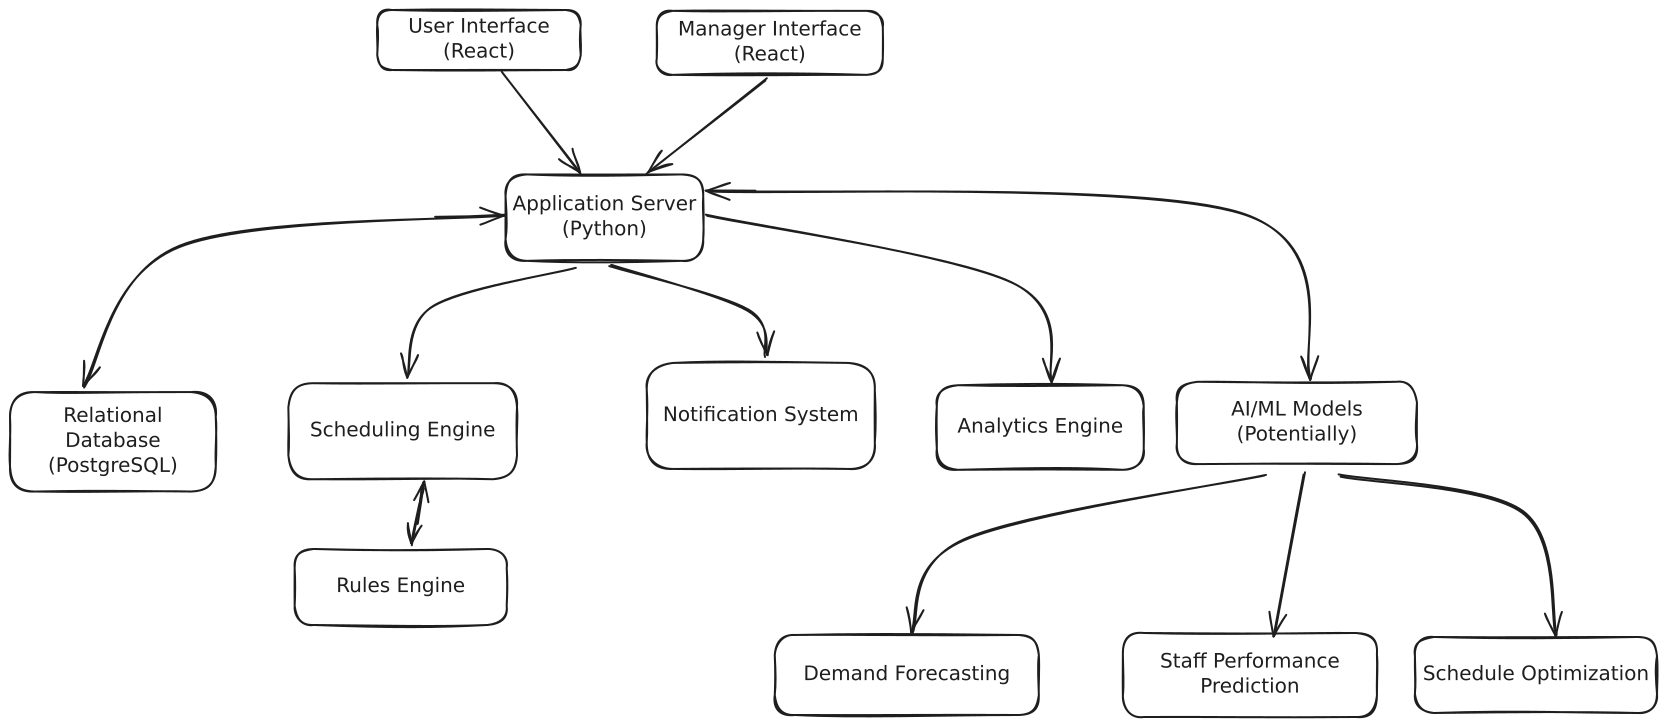
\includegraphics[width=\linewidth]{UMLDiagrams/sys_architecture_v2.png}
    \caption{System Architecture}
    \label{fig:sys-arc}
\end{figure}

The system architecture is made up of many different components and systems surrounding the main application server. The components includes:
\begin{itemize}
    \item {
    \textbf{User Interface: }The User Interface for employees developed with React Js. 
    }
    \item {
    \textbf{Manager Interface: }The User Interface for managers developed with React Js.
    }
    \item {
    \textbf{Relational Database: }The main database developed with PostgreSQL or SQLite (Not much differences between either).
    }
    \item {
    \textbf{Scheduling Engine: }The system for schedule creation with main logic developed with JavaScript and Python (Reasoning will be explained in Section \ref{sec:programming-languages}).
    }
    \item {
    \textbf{Rules Engine: } The system that works closely with the scheduling engine to implement all the constraints and rules such as max working hours (hard constraints) and preferred shift hours (soft constraints). This will also be developed with JavaScript and Python.
    }
    \item {
    \textbf{Notification System: }The system that sends notifications to managers for conflict management and leave requests received. For employees, it will send the results of leave requests as well as when there are changes to their shifts.
    }
    \item {
    \textbf{Analytics Engine: }The system that calculates all the KPI and analyses data of employees to improve the algorithms. This system is a lower priority task as it is not one of the main functionalities.
    }
    \item {
    \textbf{AI/ML Models: }This is the AI/ML models that can help with predicting employee tardiness patterns, demand prediction and other data that can help with improving the algorithm for better accuracy. This system is not a functionality, it is an extra component that will be made if there is extra time after the high priority tasks.
    }
\end{itemize}
All those components will connect to the main application server which serves as an API between every component and be the foundation of our whole system.\\

\section{UML Diagrams}
\subsection{Use Case Diagram}
\begin{figure}[H]
    \centering
    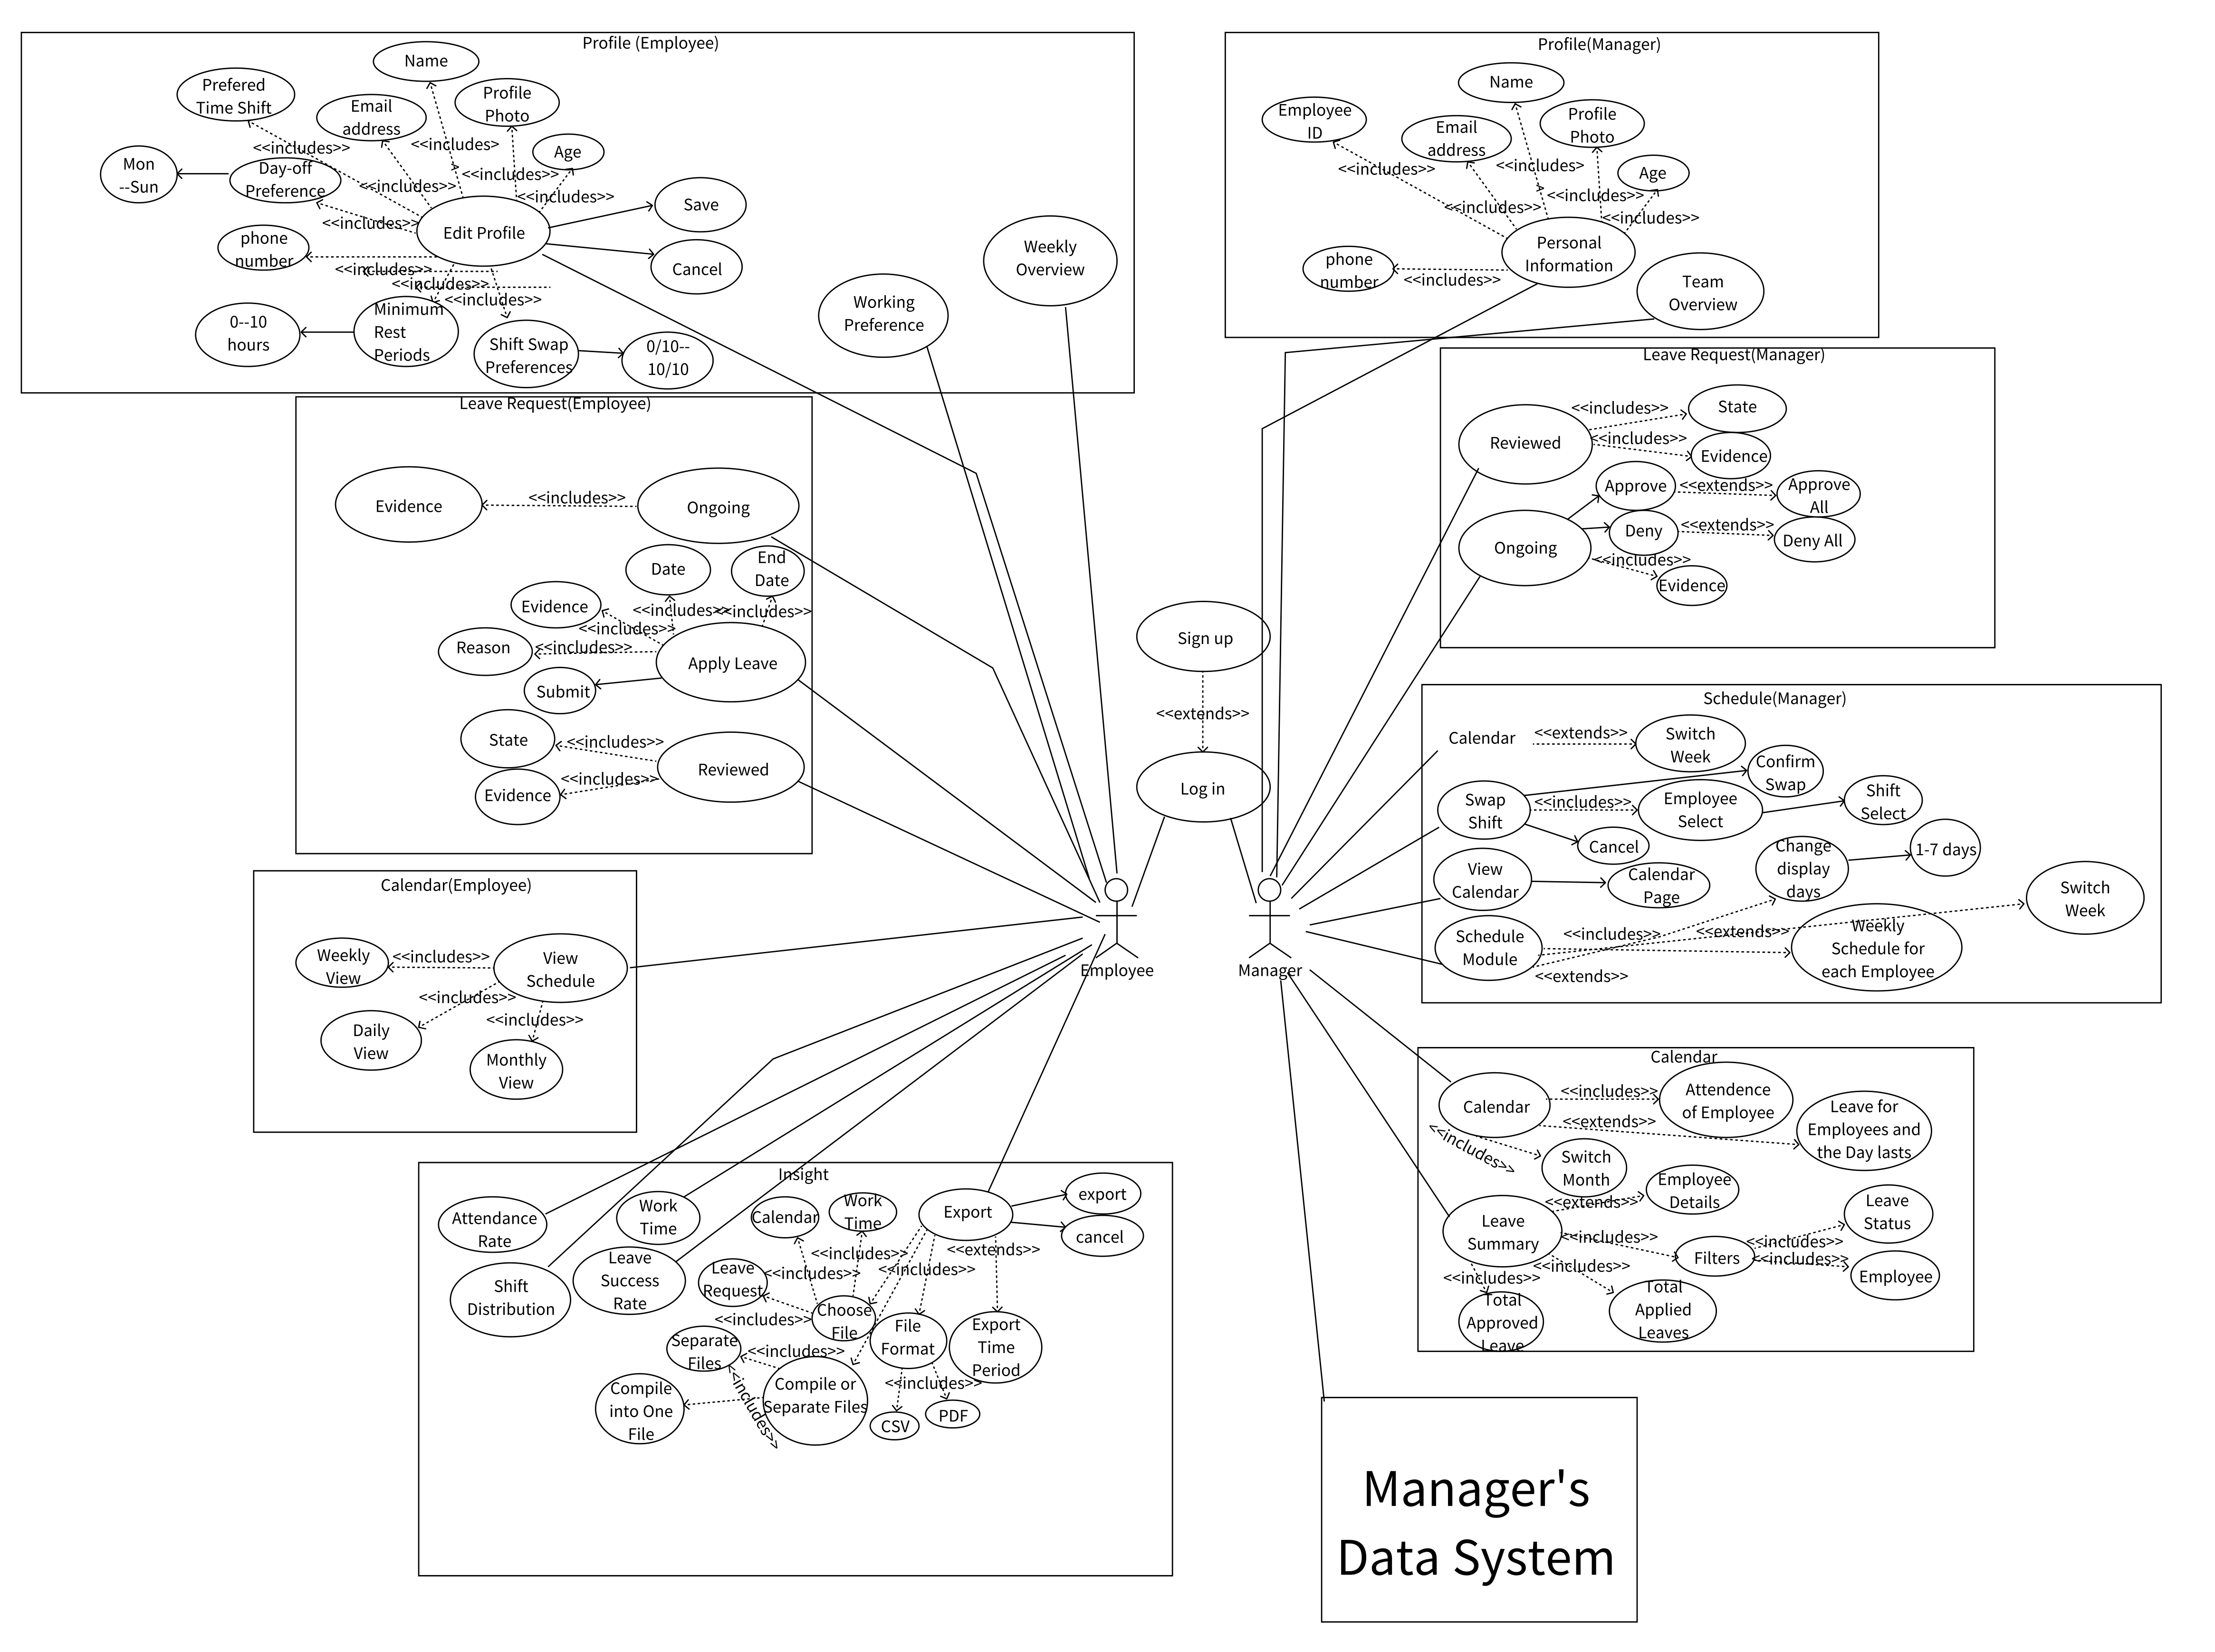
\includegraphics[width=\linewidth]{UMLDiagrams/UseCase1.png}
    \caption{Use Case Diagram}
    \label{fig:use-case-1}
\end{figure}

\begin{figure}[H]
    \centering
    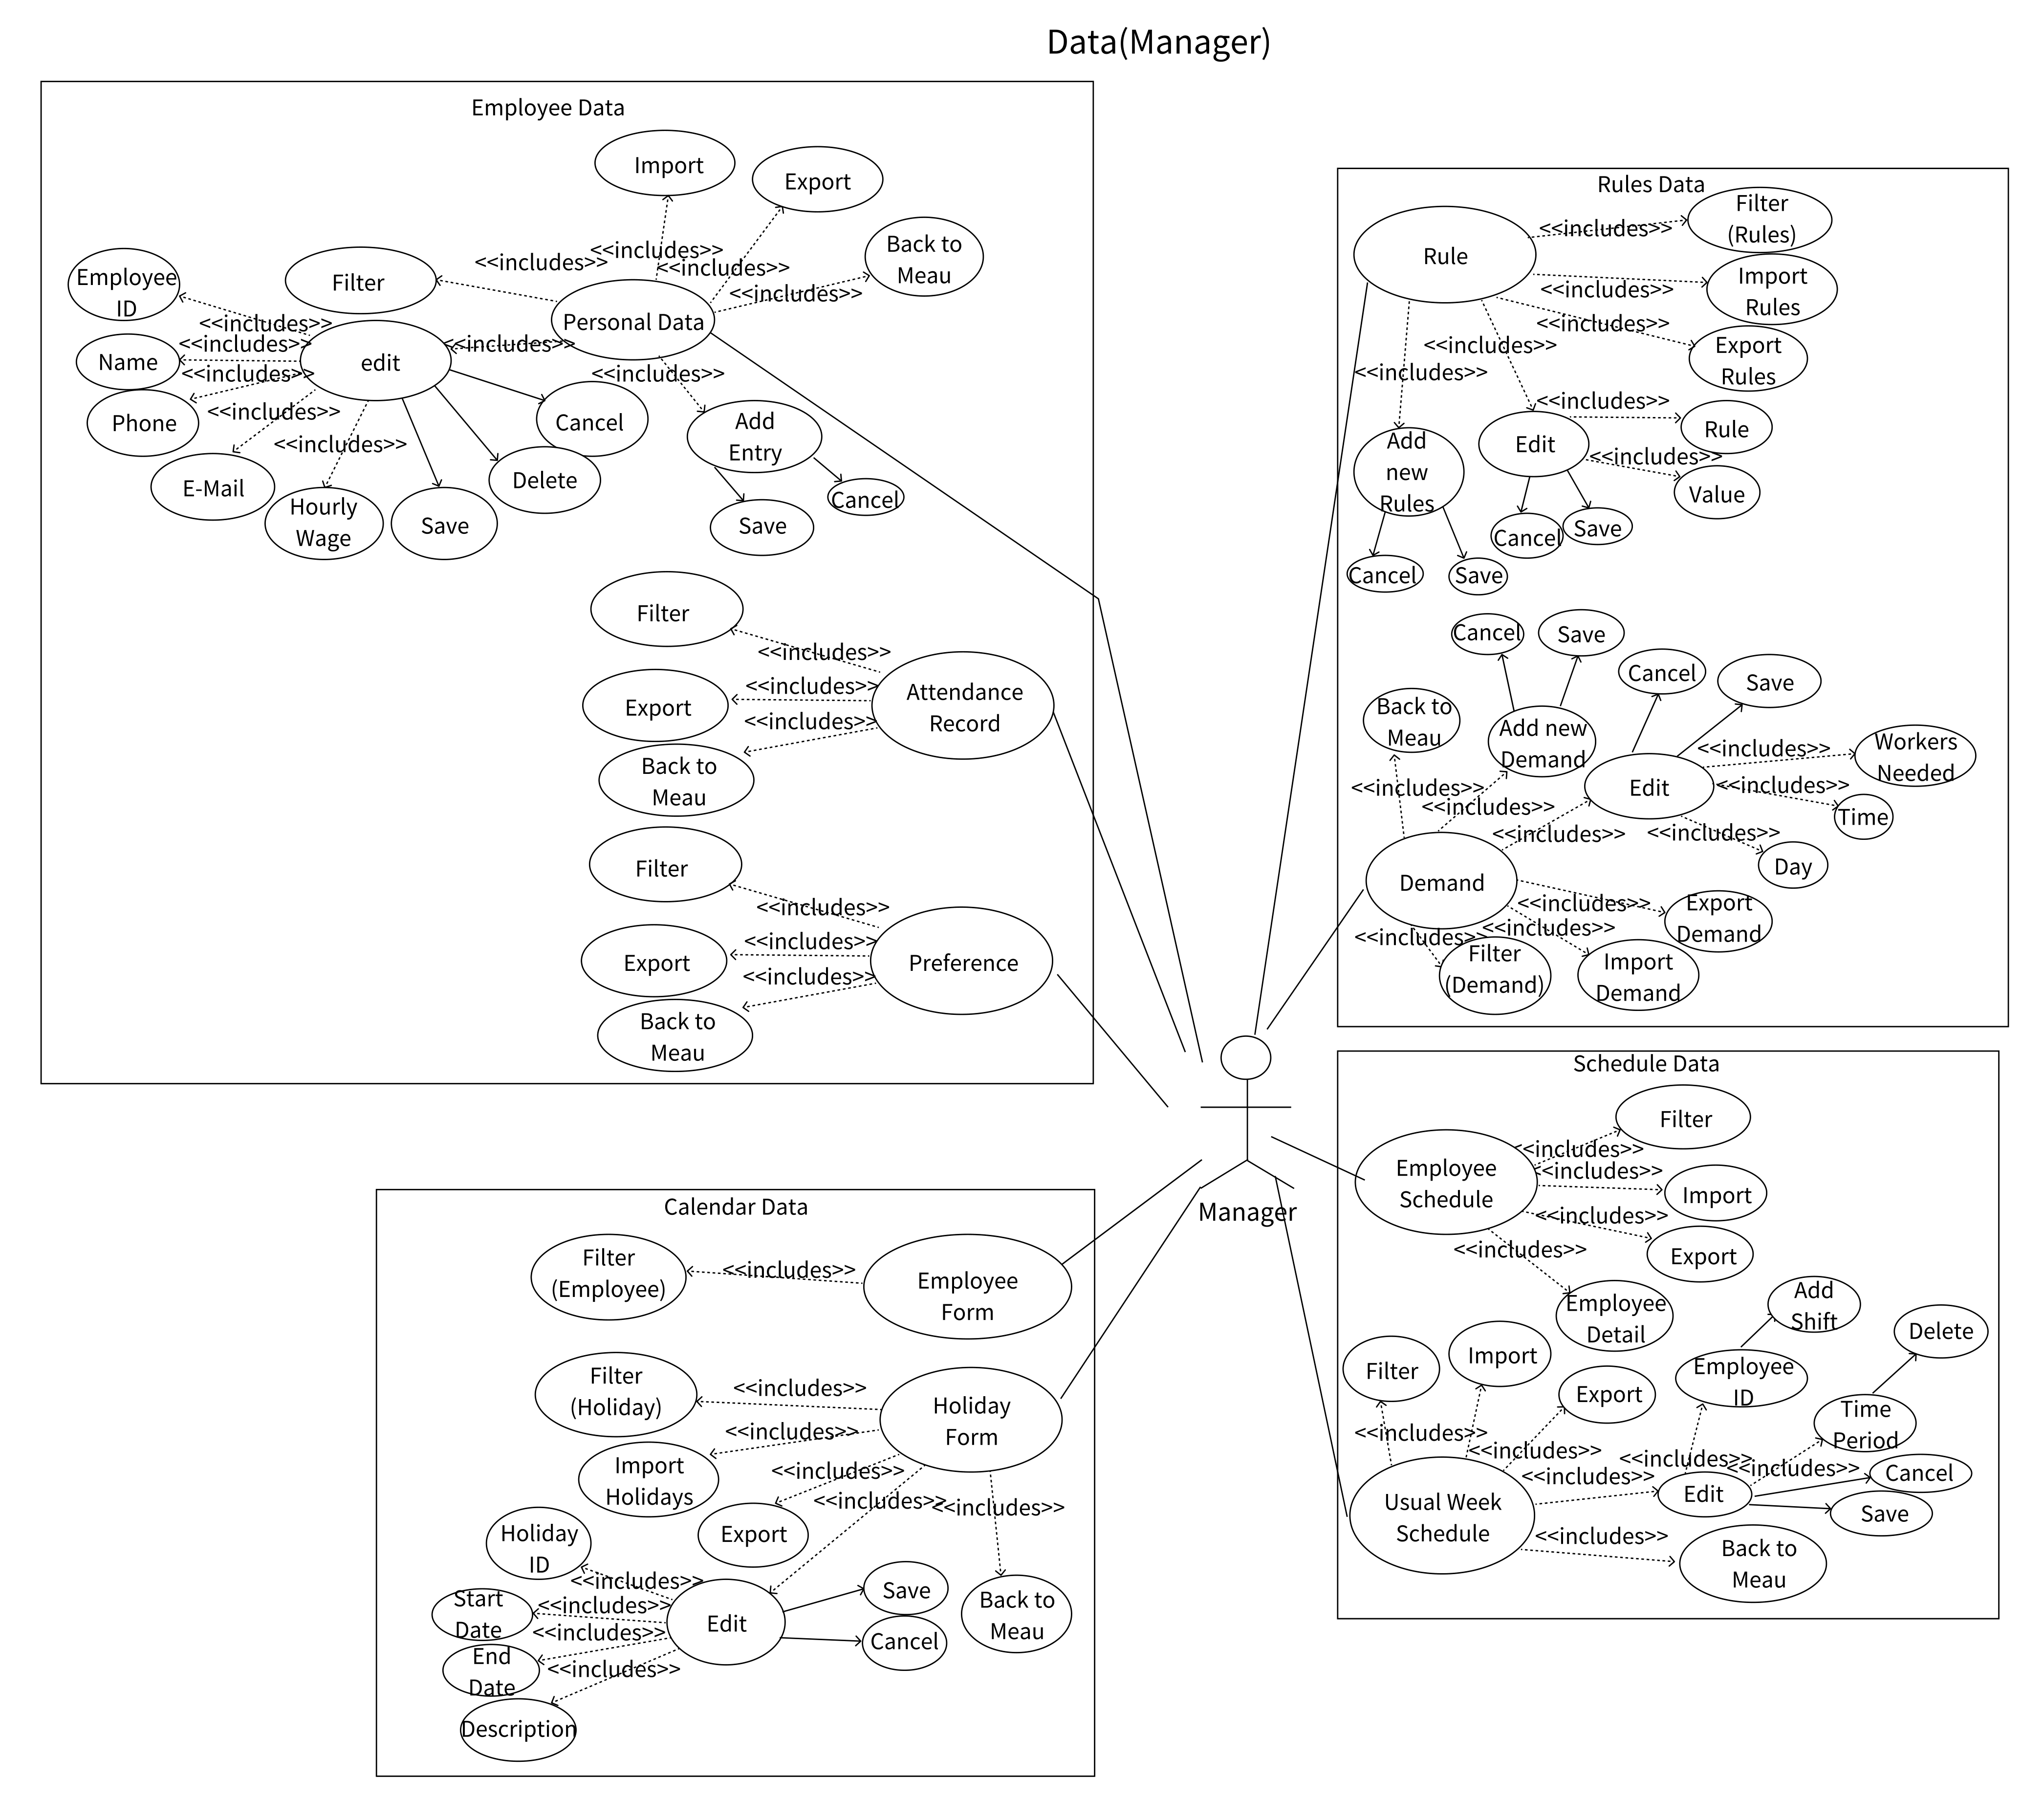
\includegraphics[width=\linewidth]{UMLDiagrams/UseCase2.png}
    \caption{Use Case Diagram - Manager Data}
    \label{fig:use-case-2}
\end{figure}

The Use Case Diagram in Figure \ref{fig:use-case-1} shows the different functions and permissions of the dynamic scheduling system in the employee and manager roles. Employees' functions include calendar viewing, check-in, submitting leave requests,  and exporting insights/calendar. The manager's functions include viewing and editing employee schedules, viewing calendar detailing employee leaves and holidays, dealing with leave requests, making shift adjustments, setting up rules for employees to go to work (e.g. maximum working hours), and importing and exporting other data. Both employees and managers first need to sign up for an account and then log in to the system.\\

Both Employees and Managers have a profile system, leave request system, calendar system and insights (for employee)/data (for manager) system. Manager has the schedule system additionally.\\

In the profile system, both the employee and manager have the same personal information screen, which includes information such as name, phone number, etc. The employee's profile system also includes a Working Preference and Weekly Overview section, where the user can view their shift and fill in the working preference to make it easier for the system and managers to arrange more reasonable time slots for their shifts (Figure \ref{fig:employee-profile}). In contrast, the manager's profile system has a team overview, which makes it easy for each manager to view information about their employees and their work (Figure \ref{fig:manager-profile}).\\

In the leave request system, the manager can view the leave requests in the reviewed or ongoing states and can approve or reject leave requests in the ongoing state with evidence. To make it easier for the manager to process leave requests efficiently, we have also added a batch-processing feature (Figure \ref{fig:manager-on-leave-request}, Figure \ref{fig:manager-rev-leave-request}). Employee's leave request system consists of a section where employees can view past or current leave requests and a section where employees can fill out a leave request that includes the time, reason, and evidence for their leave (Figure \ref{fig:employee-on-leave-request}, Figure \ref{fig:employee-rev-leave-request}). \\

In the calendar system, the employee keeps track of their scheduling through a calendar that adjusts the number of days displayed (day, week, month) (Figure \ref{fig:employee-daily-schedule}, Figure \ref{fig:employee-weekly-schedule}, Figure \ref{fig:employee-monthly-schedule}). The manager has a different calendar system compared to the employee, they have a large calendar that allows them to see the attendance of the employee and also the holiday remaining for the employee on leave. In addition, the manager also has a leave summary that includes filters, which not only filter what is shown on the calendar for the manager but also contain employee details (Figure \ref{fig:manager-calendar}).\\

In the insight system of employees, the employee can export information for a selected period, including hours worked, attendance, days off and shift details. After a specific period has been selected, the user selects the output file format, file content and single or multiple file output through the export function (Figure \ref{fig:employee-insight-page}, Figure \ref{fig:employee-export-data}).\\

The manager's data system, as depicted in Figure \ref{fig:use-case-2}, comprises four components: Employee Data, Rule Data, Calendar Data and Schedule Data. Employee data encompasses personal information, attendance records and preferences that can be edited or added by the manager. It also allows for importing or exporting through Excel and other file formats (Figure \ref{fig:manager-employee-data-personal}, Figure \ref{fig:manager-employee-data-attendance}, Figure \ref{fig:manager-employee-data-preferences}). In calendar data, the manager can view employees' leave records and export files via Excel etc., while also being able to import and edit holiday information to remind employees of vacation dates (Figure \ref{fig:manager-calendar-data}). Rules data includes regulations that all employees must adhere to (e.g., maximum working hours), which can be edited, added or imported/exported via Excel. Additionally, it contains the number of employees required for each shift on every workday - this is editable/added/importable/exportable by the manager as well (Figure \ref{fig:manager-rules-data}). Finally, schedule data is divided into employee schedules and usual week schedules; managers may import/export each employee's schedule within their respective category (Figure \ref{fig:manager-employee-schedules-c}, Figure \ref{fig:manager-usual-schedules}).\\

In the manager schedule system, the manager can view a general overview of the scheduling of all employees for a given week through the calendar and can switch time slots. In addition, the manager can use the swap shift function, using this function they must select the employee who needs to be swapped and the shift, then fill in the employee to swap. Afterwards, the system will change shifts based on the employee's scheduling and make recommendations (if the shift swap is unreasonable). To make it easier for managers to get more detailed scheduling information, a function that switches to the calendar page is set in the system (Figure \ref{fig:manager-schedule}).\\

\subsection{Sequence Diagrams}
\subsubsection{Schedule Creation}
\begin{figure}[H]
    \centering
    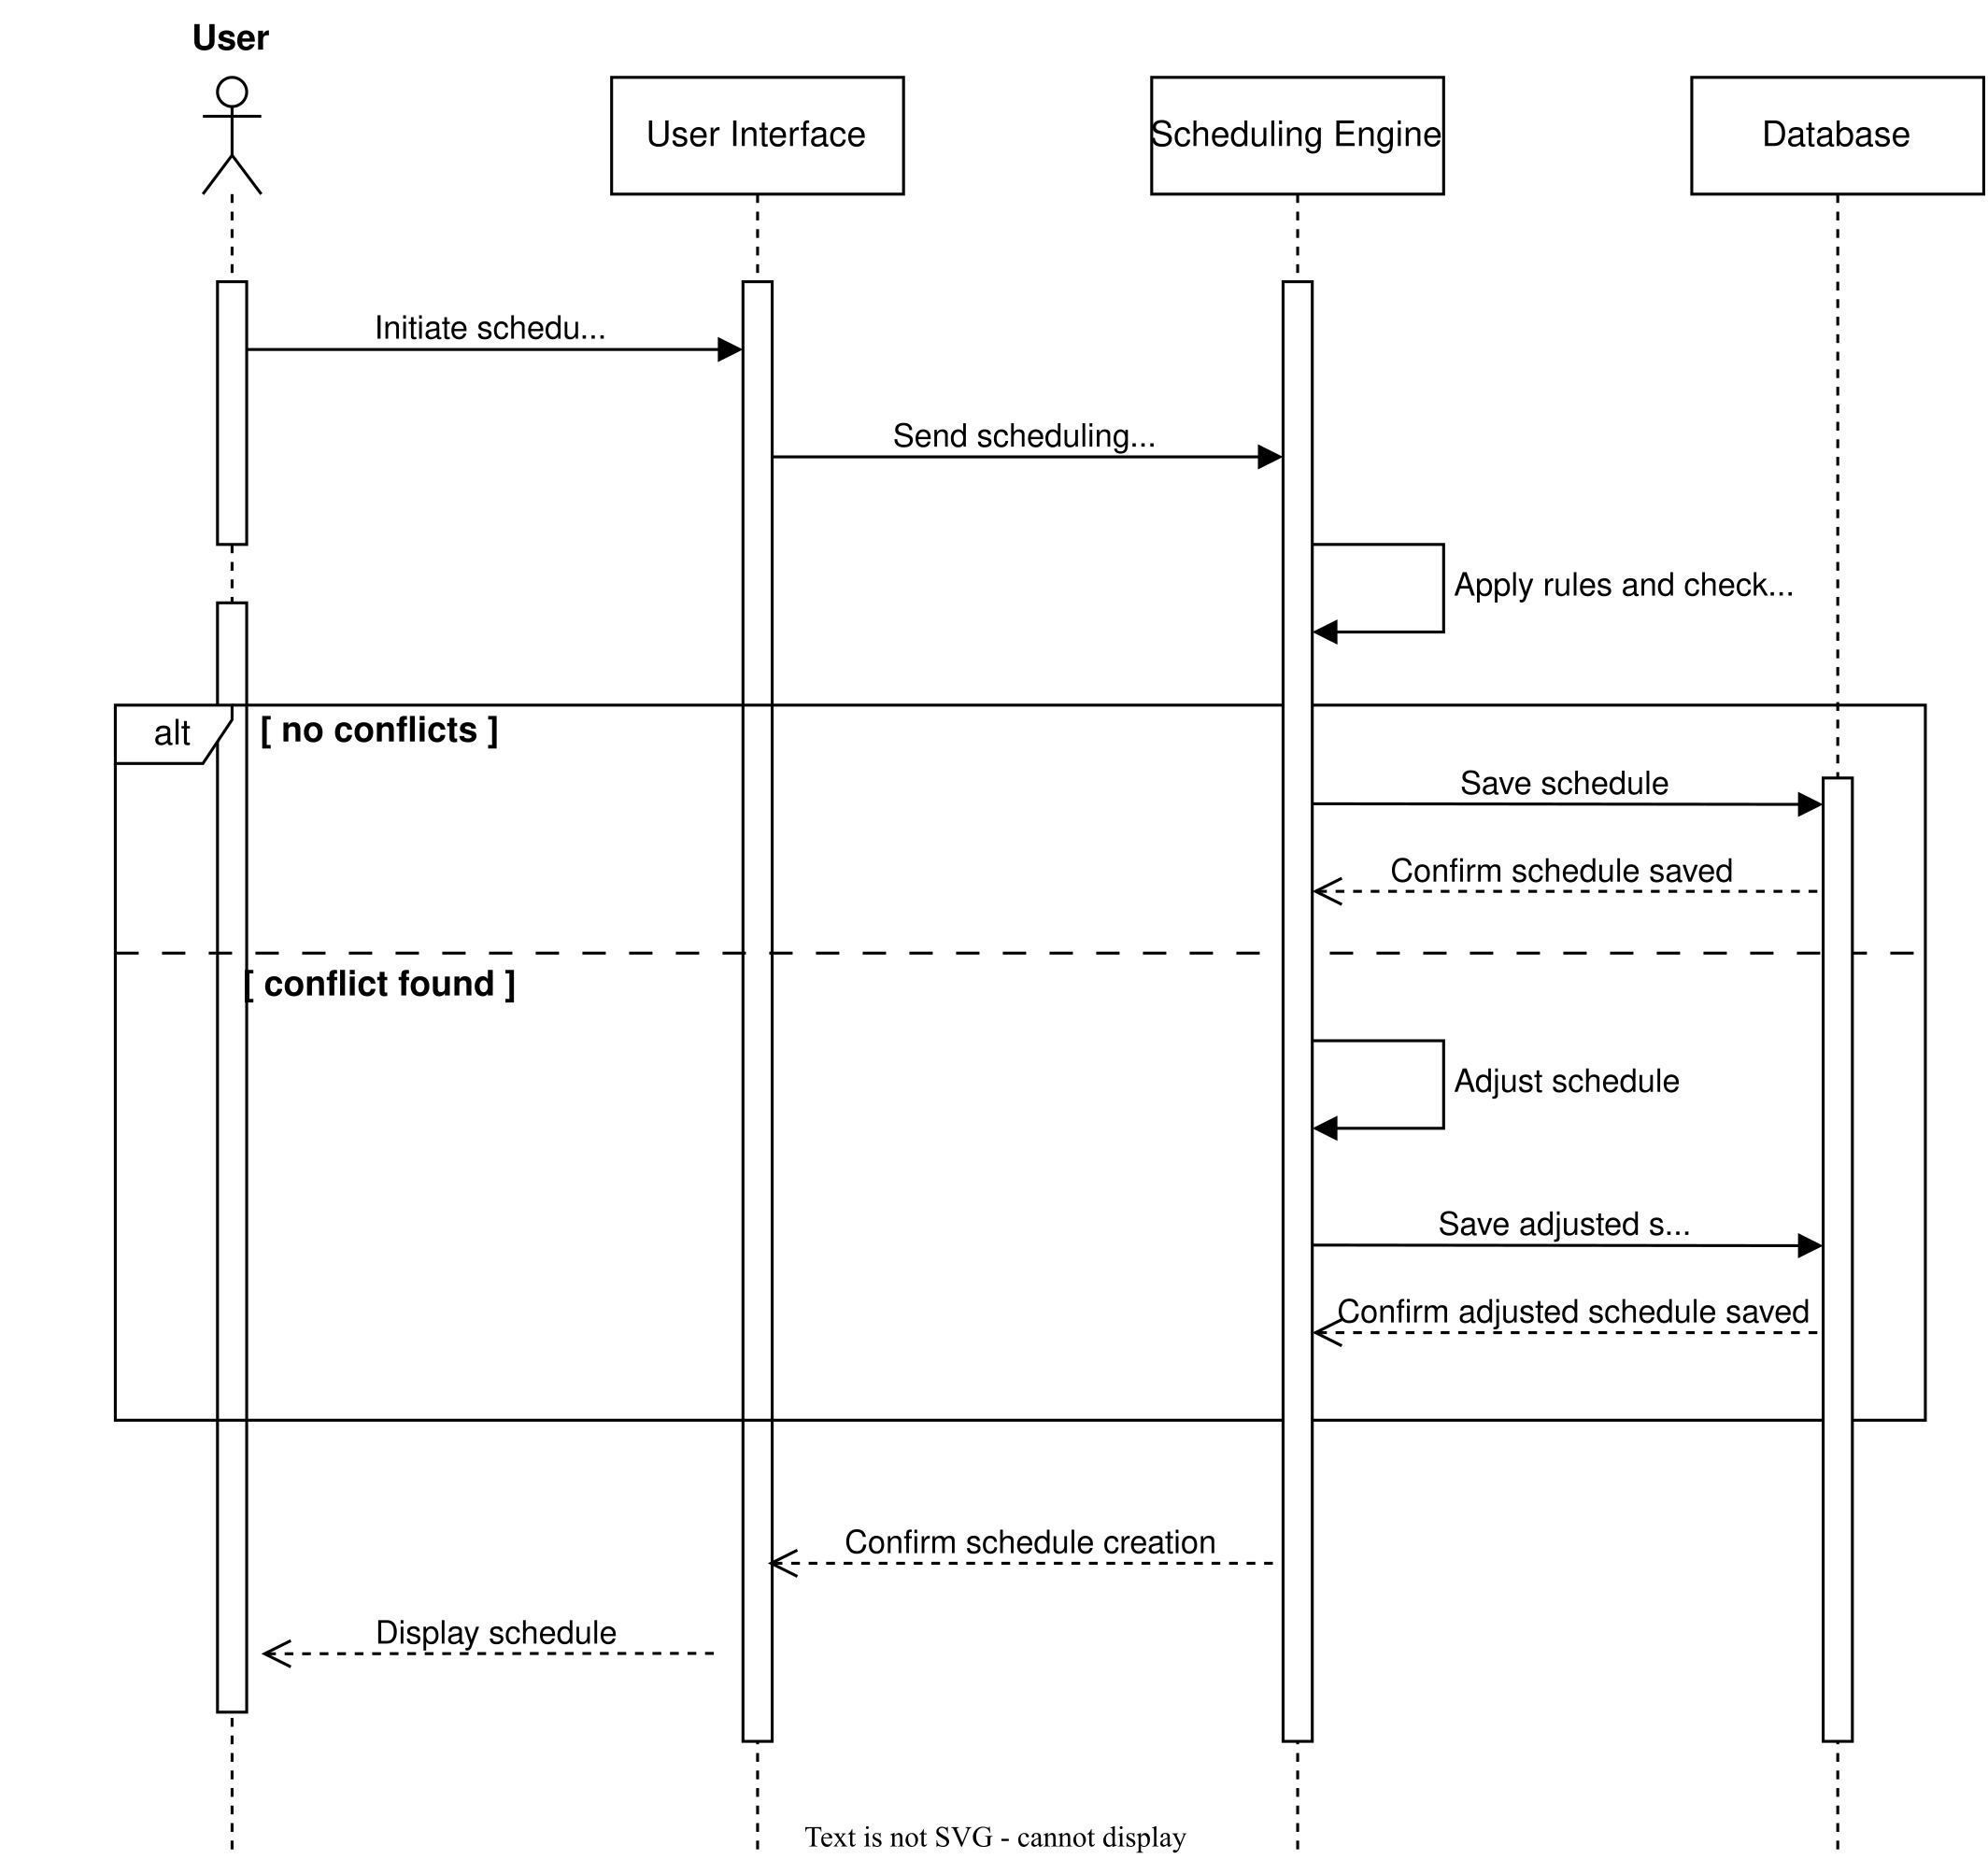
\includegraphics[width=\linewidth]{UMLDiagrams/scheduleCreation_white.jpg}
    \caption{Schedule Creation}
    \label{fig:schedule-creation}
\end{figure}
For Schedule Creation, firstly the user would initiate a schedule request. This could be either importing new data or just adding new real time data that may change the schedule. The user interface then sends a request to the scheduling engine which works with the rules engine to make a new schedule. Once everything is validated with no conflicts, it saves the schedule into the database which in return replies with confirmation. However, if there is conflict, it adjusts the schedule until there is no conflict left. Finally we send the schedule back to the user interface which displays the new schedule to the user.

\subsubsection{Staff Leave Request}

\begin{figure}[H]
    \centering
    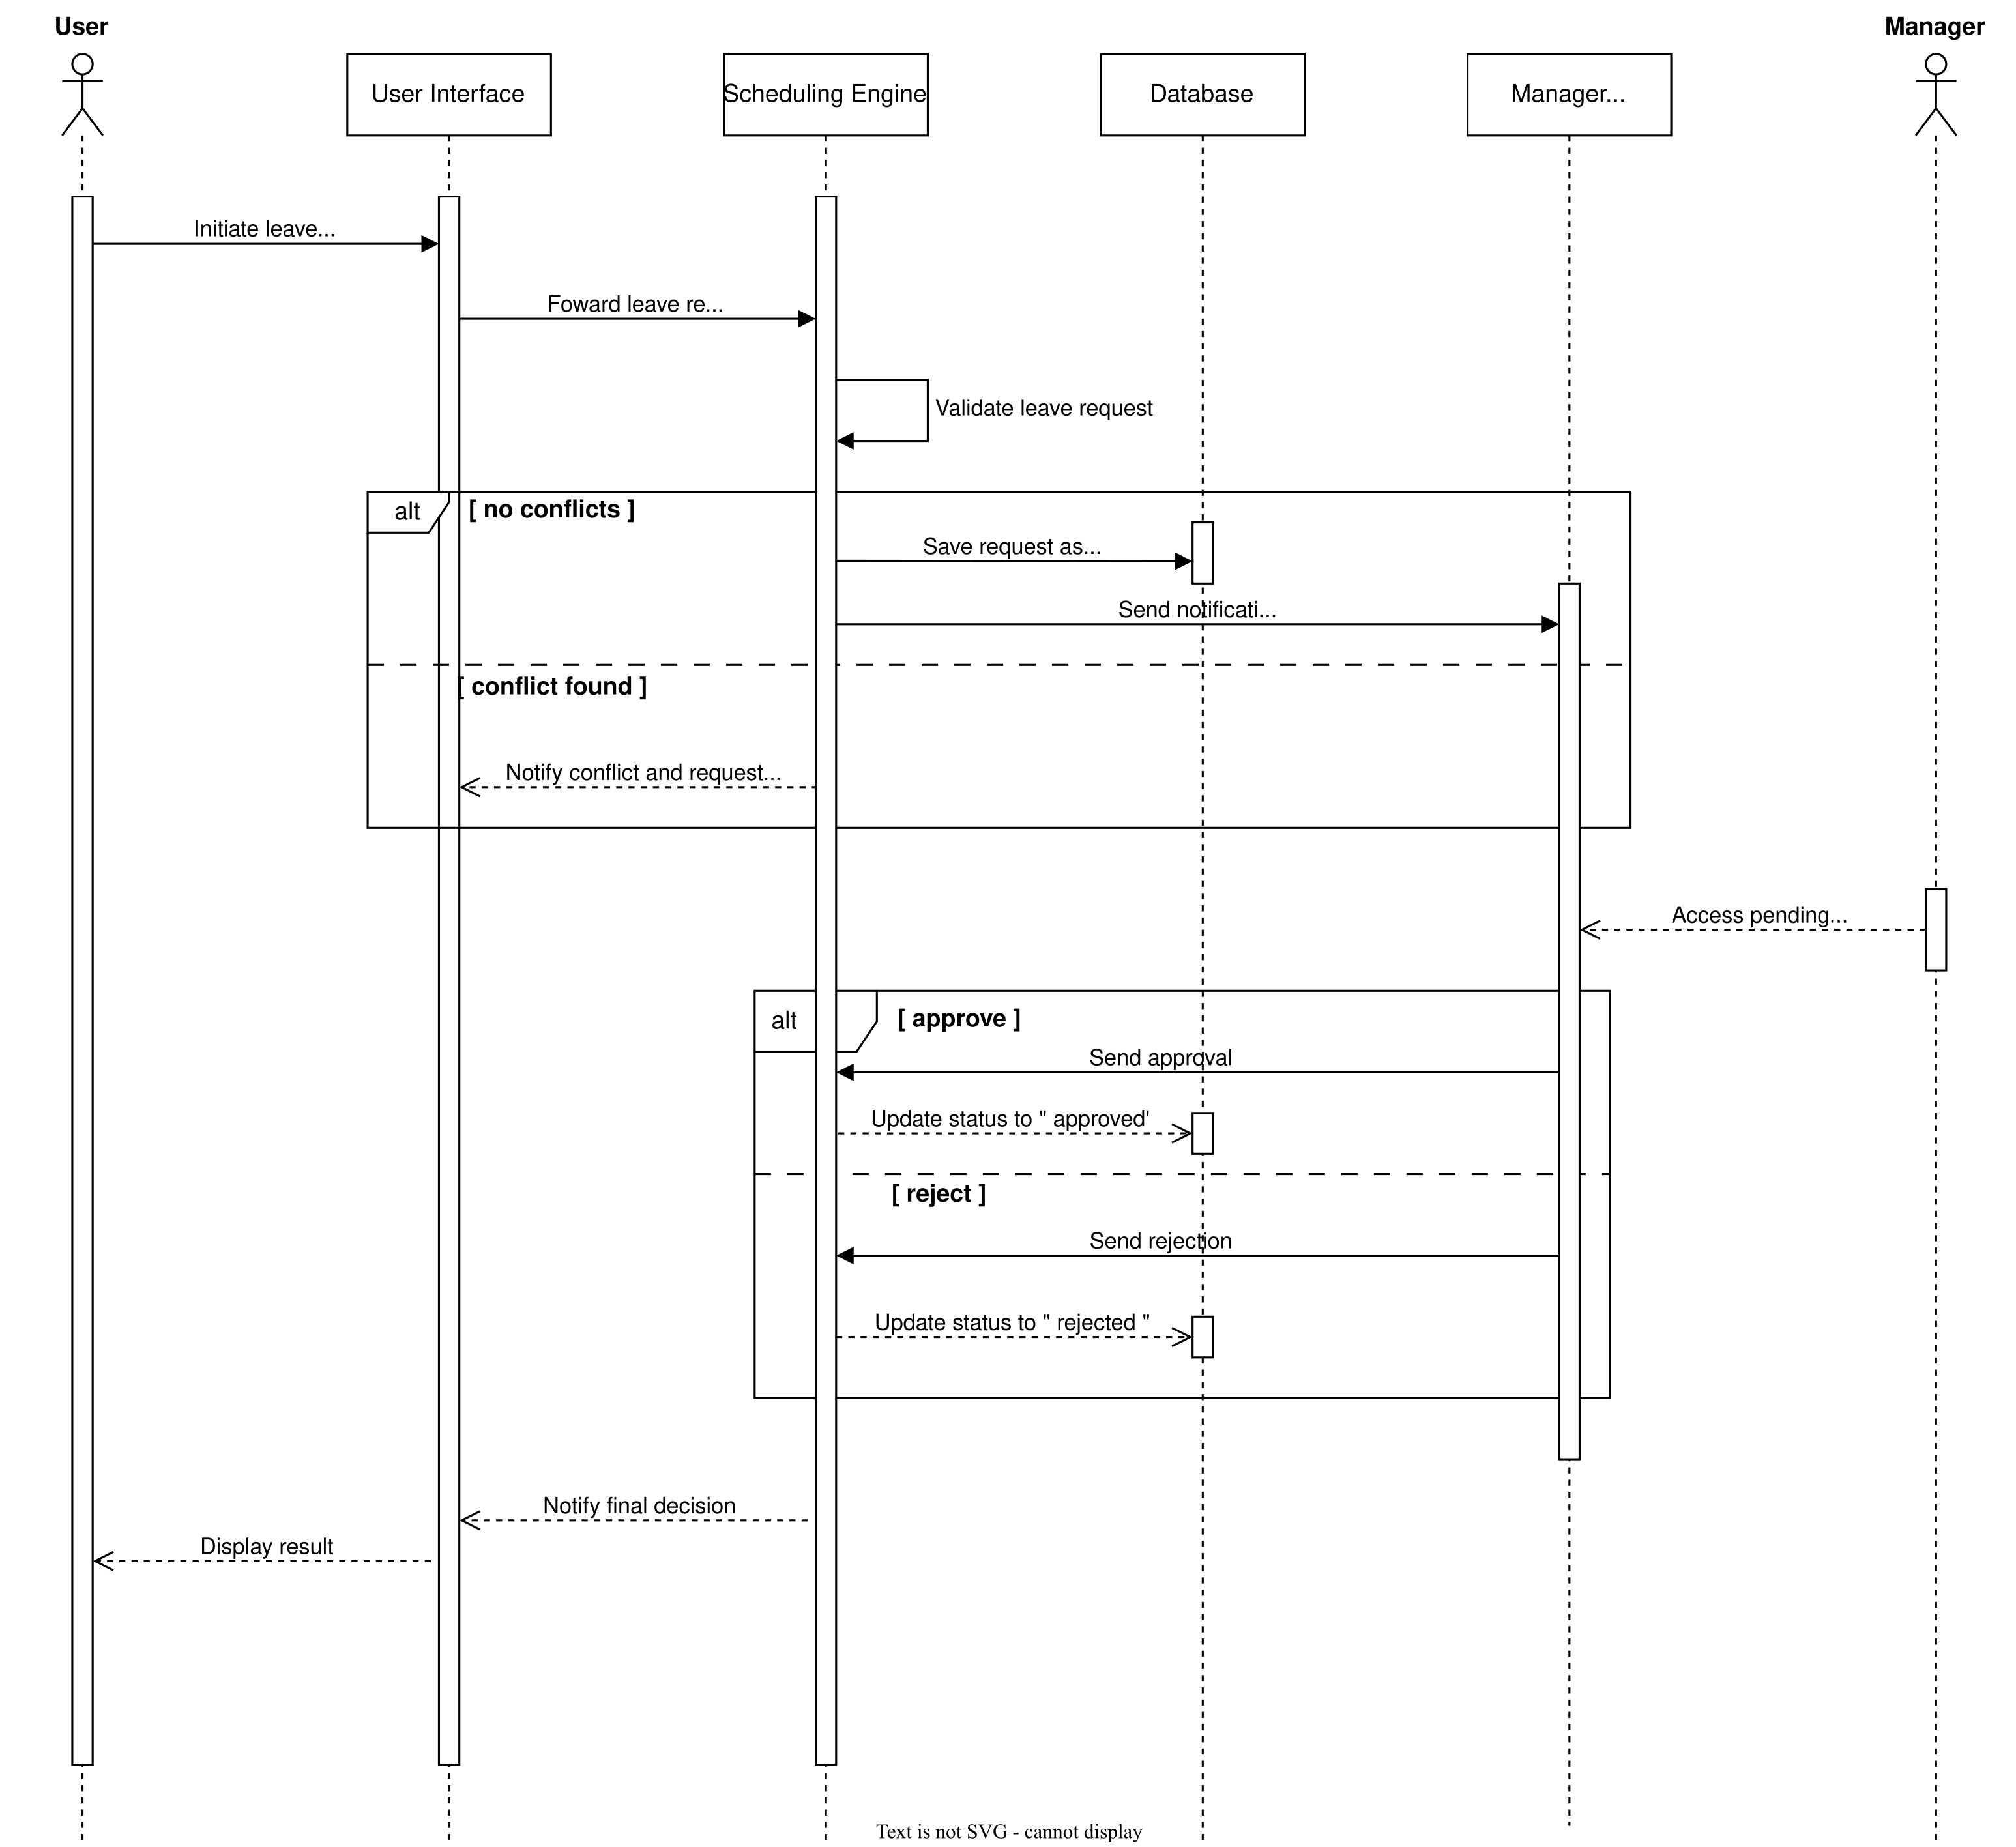
\includegraphics[width=\linewidth]{UMLDiagrams/staffLeaveRequest_white.jpg}
    \caption{Employee Apply Leave}
    \label{fig:apply-leave}
\end{figure}

For Employee Leave Requests, the employee firstly makes a request to the user interface using the apply leave form. The user interface sends the input to the scheduling engine which automatically validates the request. If the apply leave requested time has conflict, it will send a notification back to the user. If the validation is passed, the request is sent to the database which then sends to the manager. The manager will then either approve or reject the request. The decision will then be sent back to the user.

\subsubsection{User Login}

\begin{figure}[H]
    \centering
    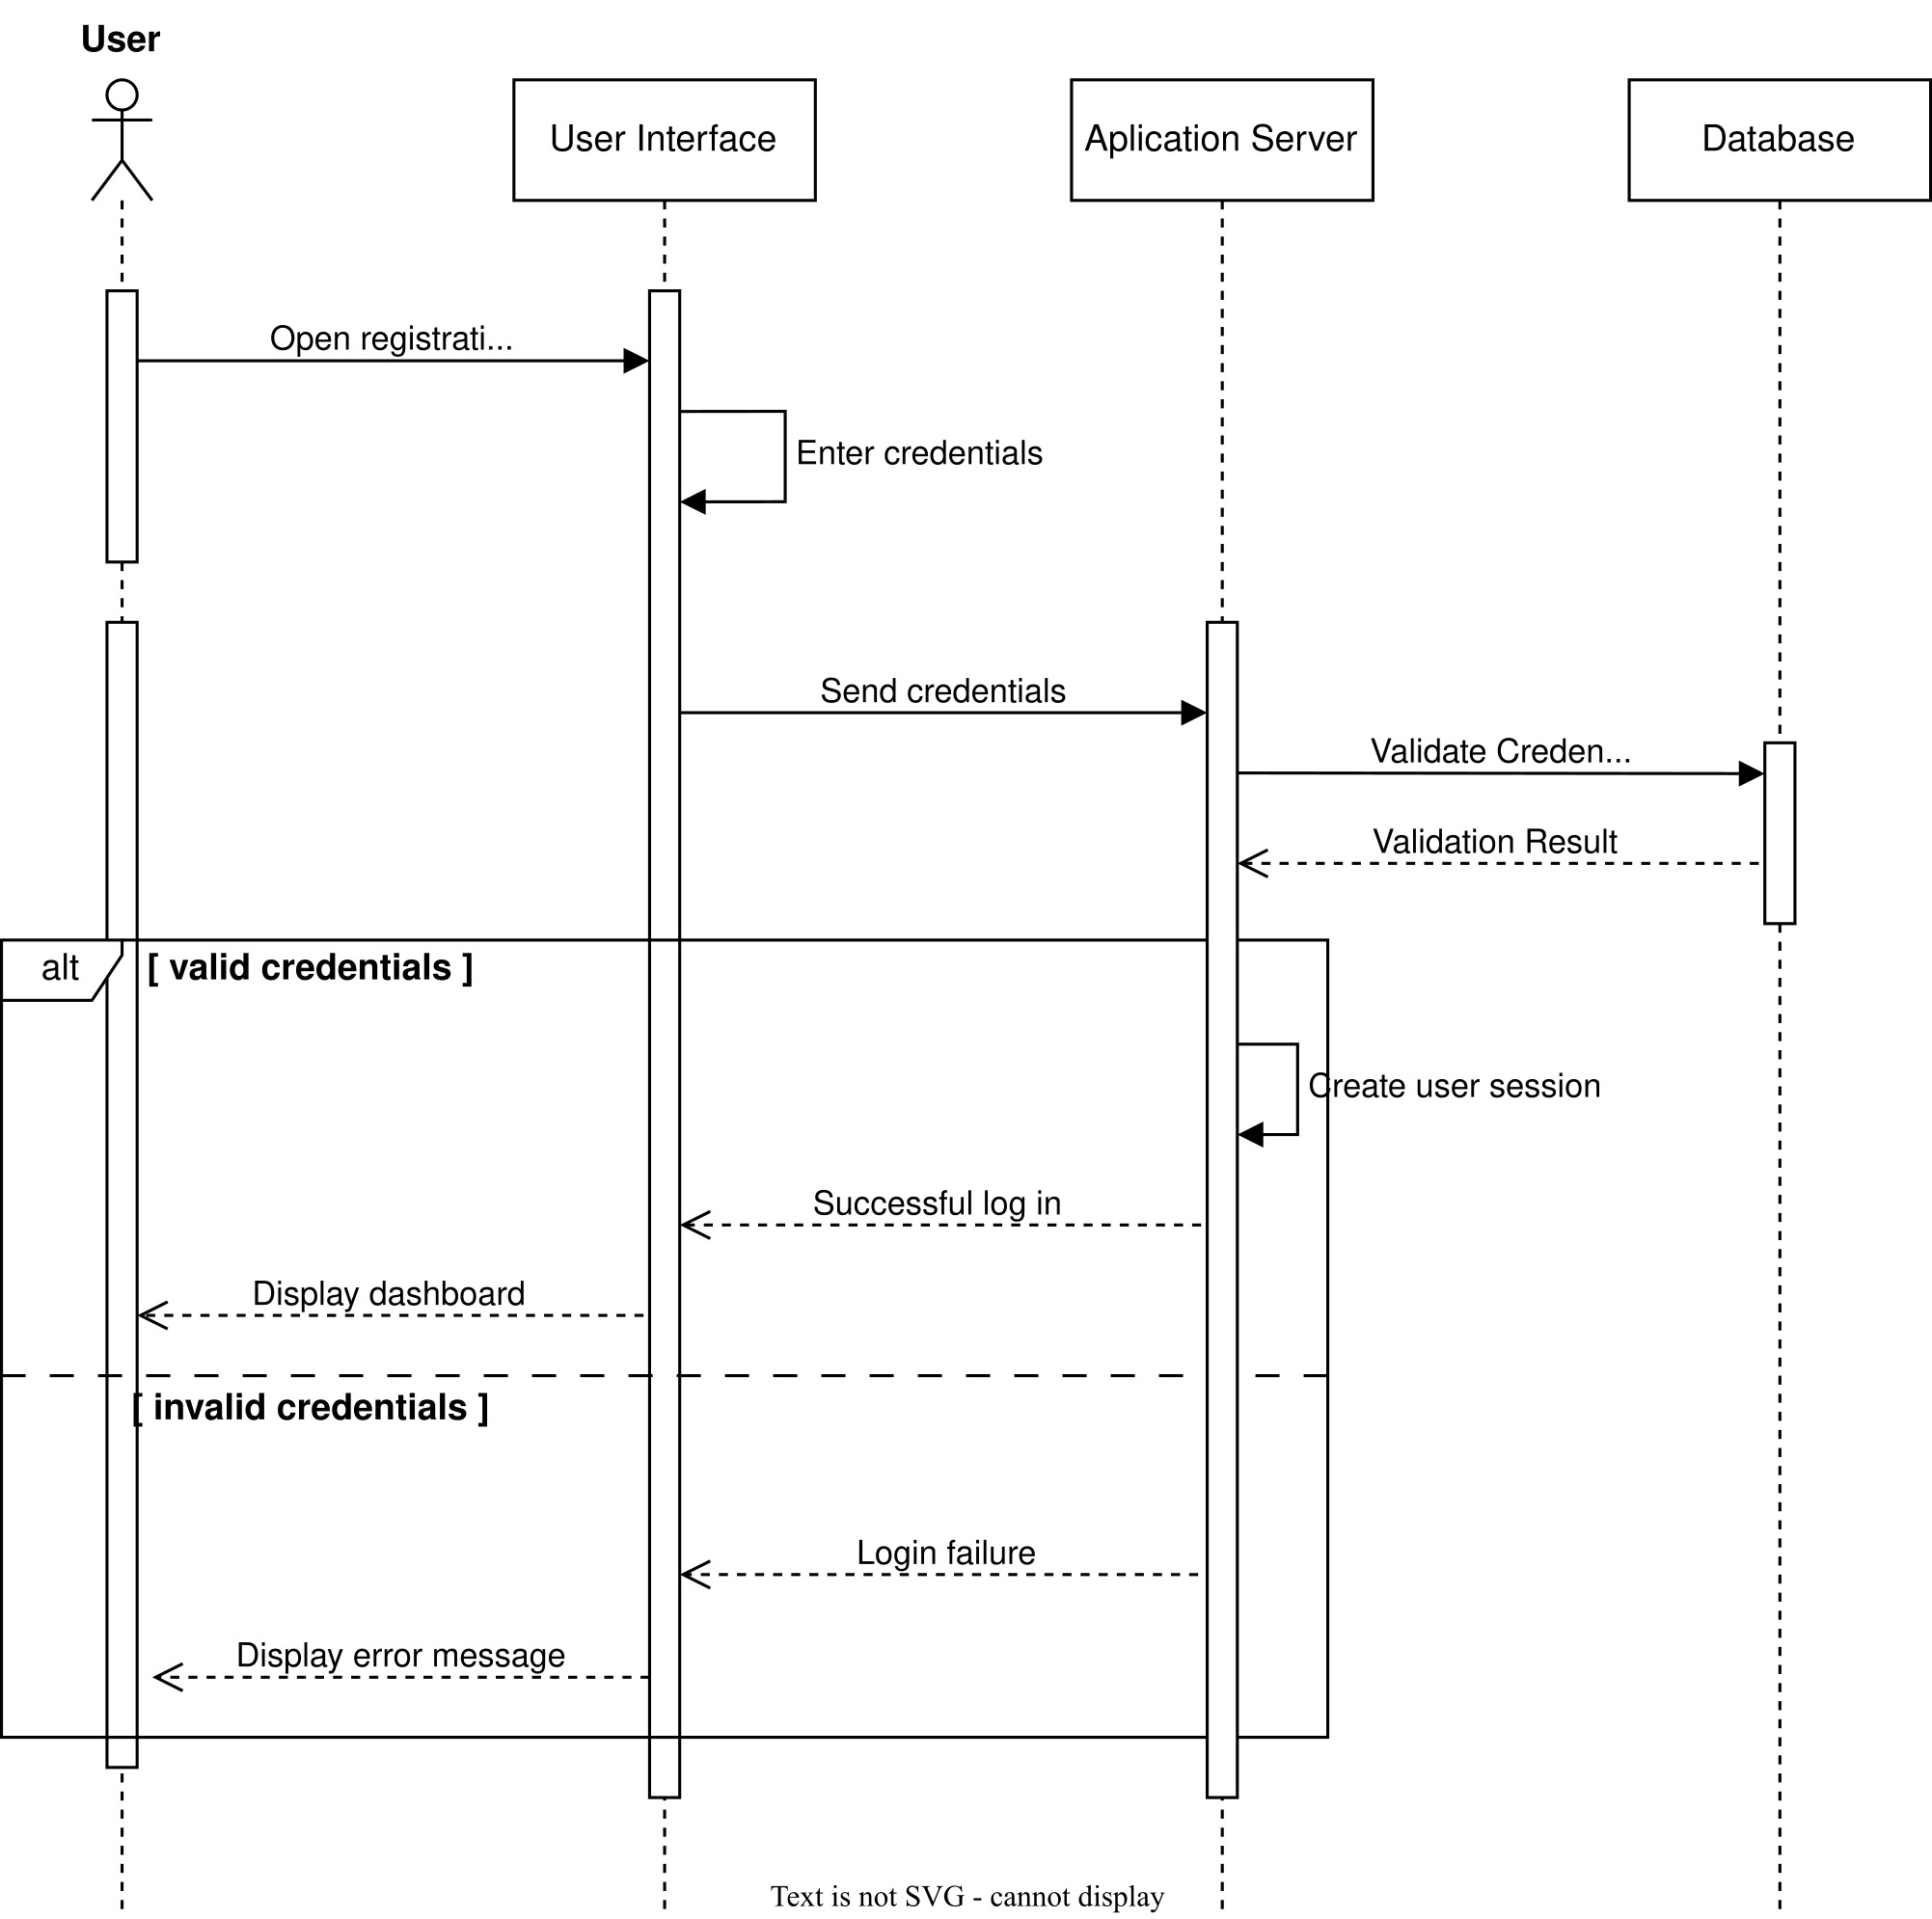
\includegraphics[width=\linewidth]{UMLDiagrams/userLogin_white.jpg}
    \caption{User Login}
    \label{fig:user-login}
\end{figure}
For User Login, the user first enter their credentials and data like username and password. Once they hit submit, the data is sent to the application server which validates the credentials with the database. If the credentials are valid, then the user will be redirected to the main dashboard. If the credentials are invalid, then the user will be denied entry and a error message will be shown to the user.

\subsection{Class Diagram}
\begin{figure}[H]
    \centering
    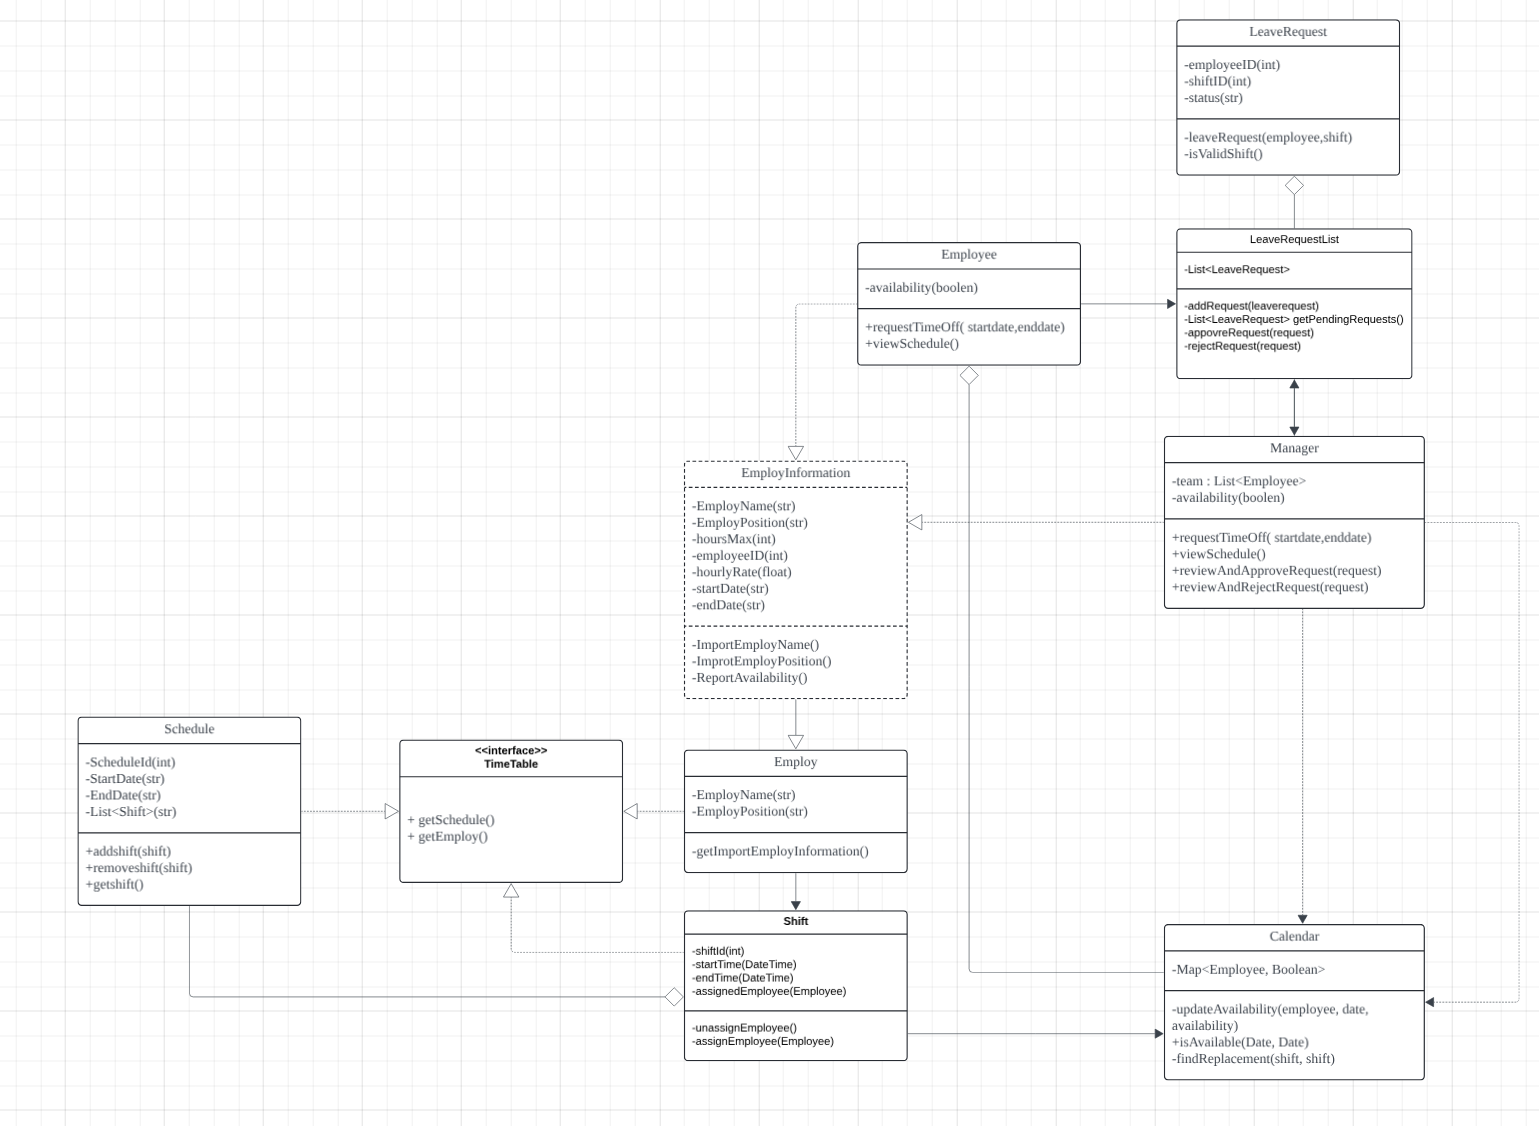
\includegraphics[width=\linewidth]{UMLDiagrams/ClassDiagram.png}
    \caption{Class Diagram}
    \label{fig:class-diagram}
\end{figure}
The class diagram shown at Figure \ref{fig:class-diagram} is the basic class diagram for the main application server. It does not include the scheduling system nor the rules system. In the class diagram, the key functionalities are shown for the two users. For employees, they are able to request time off as well as view their own schedule. Not only that, the employees are also able to indicate their availability. For managers they are able to review leave requests sent by the employees and able to view schedules as well. For now this class diagram achieve the bare minimum thus not including import/export data or being able to check in. This class diagram focuses on providing a dynamic scheduling system without additional features.


\chapter{User Interface Design}

\section{User Interface (UI)}
The UI design of this Dynamic Restaurant Staff Scheduling Tool aims to provide a clear and convenient experience for users when browsing and interacting with schedules. The target audience includes the restaurant manager, whose primary need is to be able to manage employees’ schedules, and restaurant employees, whose primary need is to view their own schedules and apply for leave.\\

\section{UI Designs}
This section outlines the evolution of UI design and the enhancements made to improve user experience.

\subsection{Initial Design}
\begin{figure}[H]
    \centering
    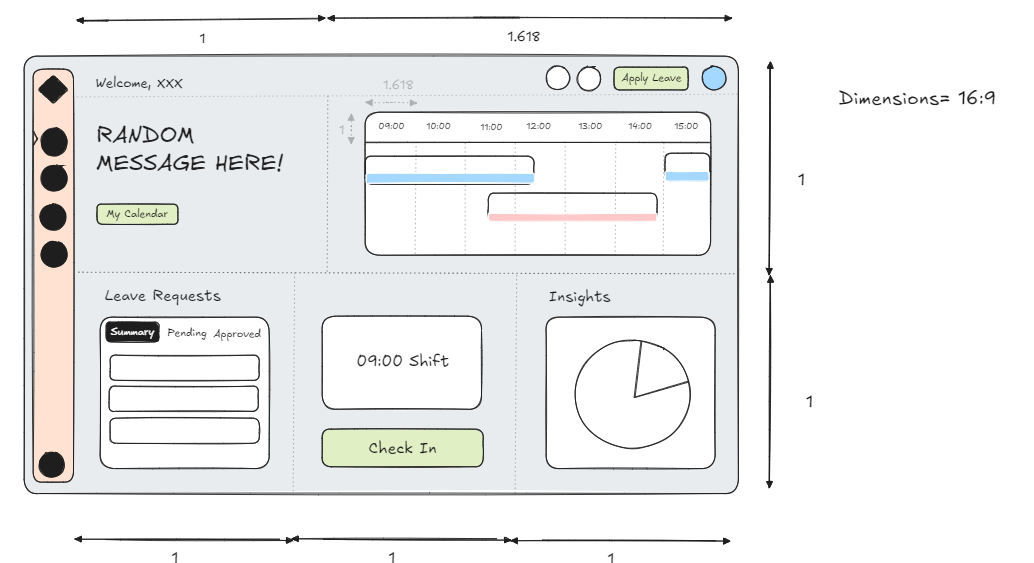
\includegraphics[width=\linewidth]{images/InitialDesign.png}
    \caption{Initial Design}
    \label{fig:initial-design}
\end{figure}

The theme and general look of our application was built on the initial design shown in Figure \ref{fig:initial-design}. This design was made using the website excalidraw, an online diagramming and brainstorming tool \citep{excalidraw}. In terms of color matching and accessibility considerations, our team chose a minimalist color scheme, using low-saturation colors to highlight the text on the web page. The web pages are mainly composed of white, gray, red and green, which avoids color clutter without being too monotonous, and can effectively distinguish different functional sections.

A study done by \citet{nikolic2011effect}, shown that younger people tend to prefer simpler shapes like triangles with the golden ratio and older consumers prefer more complicated shapes like hexagonal with the golden ratio which might be explained by the Gestalt psychology. Most restaurants hires workers around the age of 18 to 24 \citep{nationalrestaurantassociation2024demographics}. This meant that they are not more likely to prefer a complicated shape rather than a simple shape. Thus, a rectangle with the golden ratio, which was used extensively in our design, can be said to be neither too simple nor too complex.\\

\subsubsection{Initial Design Board}
\begin{figure}[H]
    \centering
    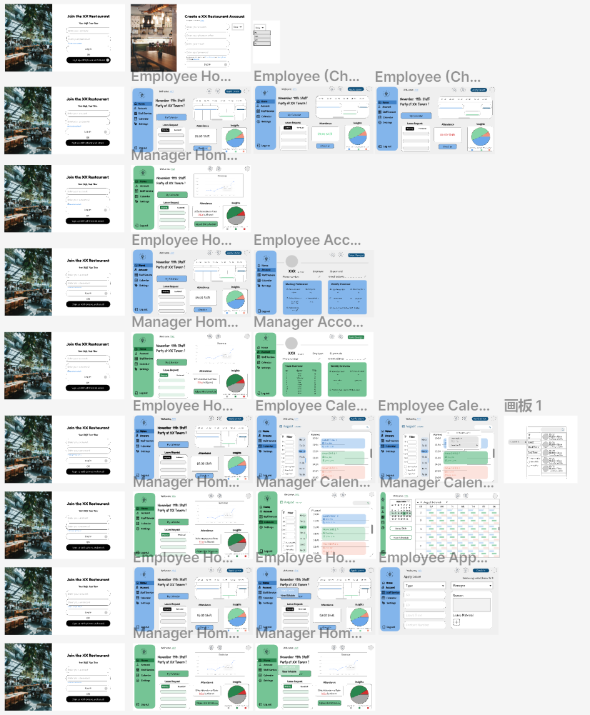
\includegraphics[width=1\linewidth]{images/design-board.png}
    \caption{Design Board}
    \label{fig:design-board}
\end{figure}

Figure \ref{fig:design-board} shows the design board made by our design team. By combining the color and dimensions of the initial design and the designs shown in the design board, allows us to achieve an appealing web application design shown in Sub-Section \ref{subsec:implemented-features}.

\subsection{UI Design Principles}
Our team’s design goal is usability, which ensures a clean, intuitive interface with straightforward navigation, and responsiveness. The styling was integrated with the components by the module CSS, creating flexible layout components, and dynamically resizing charts and tables, which enabled the interface to adapt to a variety of screen sizes, ensuring a consistent experience across desktop and mobile devices (Figure \ref{fig:home-e}, Figure \ref{fig:home-c}). In other words, a responsive layout enables the system to be more inclusive and adaptable, which enhances user experience and engagement.\\

\begin{figure}[H]
    \centering
    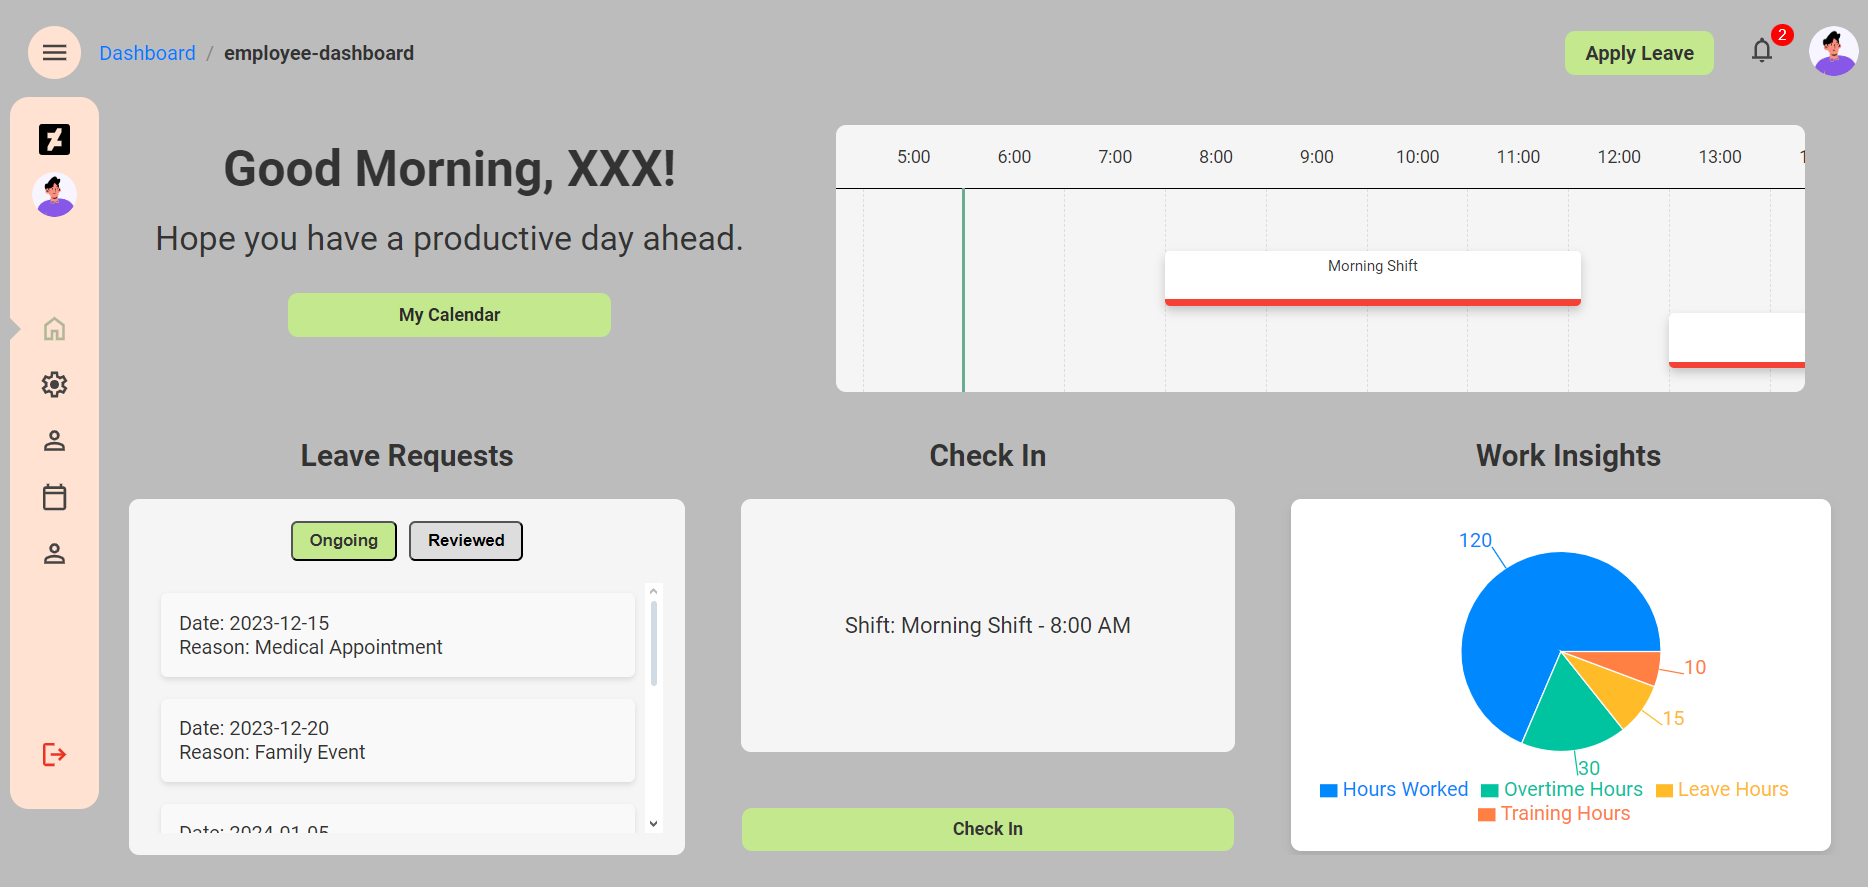
\includegraphics[width=0.8\linewidth]{images/HomeE.png}
    \caption{Dashboard Full Width}
    \label{fig:home-e}
\end{figure}
 
\begin{figure}[H]
    \centering
    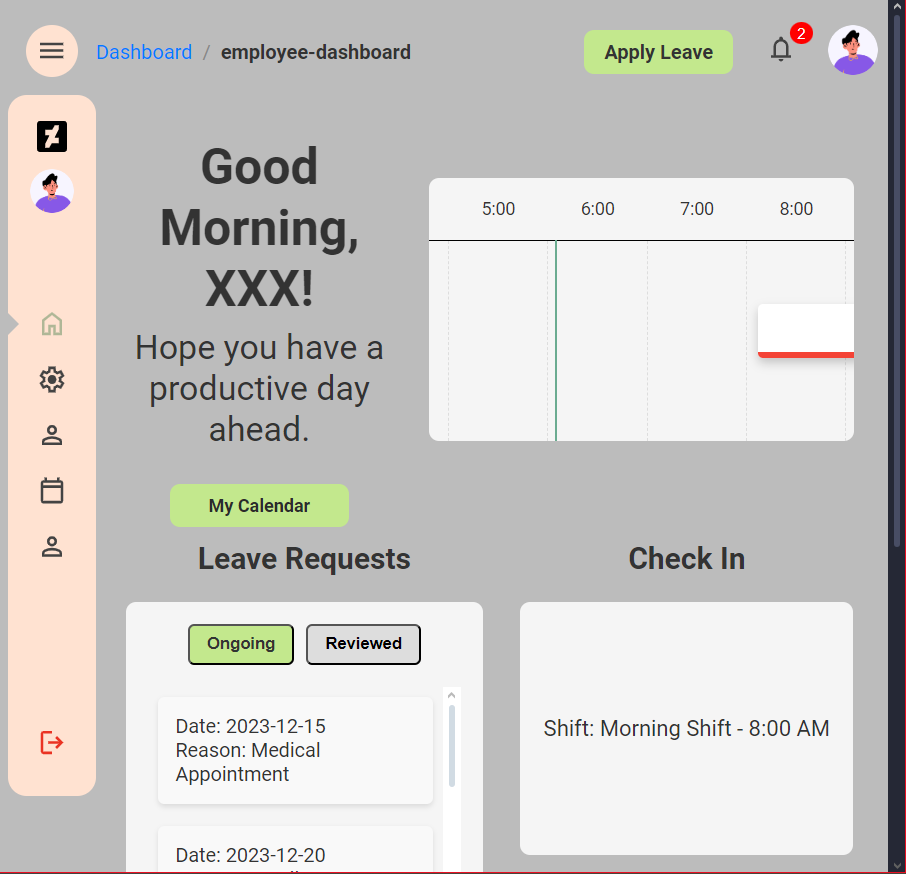
\includegraphics[width=0.65\linewidth]{images/HomeC.png}
    \caption{Dashboard Half Width}
    \label{fig:home-c}
\end{figure}

For typography, our team chose the “Roboto” font (Arial and Helvetica as backup when Roboto doesn't load) because it’s easy to read on both desktop and mobile devices and has appropriate bold and size variations to highlight key points. In the web page layout, our team used a card-style layout to distinguish different functions, allowing users to find the functions they need efficiently. At the same time, the appropriate spacing between images and text enhances readability.\\


\chapter{Implementation Methods}

\section{Software Development Method}
Our team used Windows as the development environment due to its high level of adaptability, and Visual Studio Code as the development tool to deploy the React environment. During the development process, both React and Django/JavaScript runtime environments can be built smoothly on Windows to ensure development efficiency. The deployment process is designed to ensure cross-platform consistency. To enable the software to be used by a wider group of users, our team has also ensured support for Mac. The final Dynamic Restaurant Staff Scheduling Tool will be able to run on Windows 10, Windows 11 and Mac OS as long as they are running on a suitable web browser.\\

\section{Programming Languages}
\label{sec:programming-languages}
During implementation, our team used a variety of programming languages and technical approaches depending on the different aspects of the software.\\

In the front end, our team used ReactJs with Vite, whose componentized design facilitates high reusability and dynamic interface interactions. Furthermore, the high-performance development environment provided by Vite enables the rapid development of responsive pages. \\

In the back end, our team chose JavaScript as the main language, with its compatibility with our ReactJs frontend. We understadn the struggles JavaScript might have when it comes to mathematical logic. This meant that python will also be used, with its rich libraries and frameworks (e.g. Django) that can efficiently support complex business logic processing, especially for real-time dynamic scheduling updates.\\

Finally, in the aspect of databases, we will use SQLite as the main relational database for storing scheduling information and user data according to the project requirements.\\

\section{Software and Tools}
In addition to Jira for project management \citep{jira2024projectmanagement}, our team also used other software, websites and tools in project development. GitLab is used as the version control and collaboration platform for code management. Visual Paradigm, Draw.io and Lucidcharts are used as UML diagram creation tools \citep{drawio2024diagramming} \citep{lucidchart2024diagramming}. js.design (
\begin{CJK*}{UTF8}{gbsn}
即时设计
\end{CJK*}
) and excalidraw are used to make prototypes and UI designs \citep{jsdesign2024tool} \citep{excalidraw}.\\

\section{Results of Implementation}
This section shows the progress made in initial implementation of the project. It outlines the features that have been implemented, feedback received from stakeholders, challenges encountered, and the outcomes achieved so far.

\subsection{Implemented Features}
\label{subsec:implemented-features}
\subsubsection{Employee Features}
    \begin{itemize}

    \item \textbf{Schedule Visualization:} Employees are able to view their daily, weekly, and monthly schedules.

    \begin{figure}[H]
    \centering
    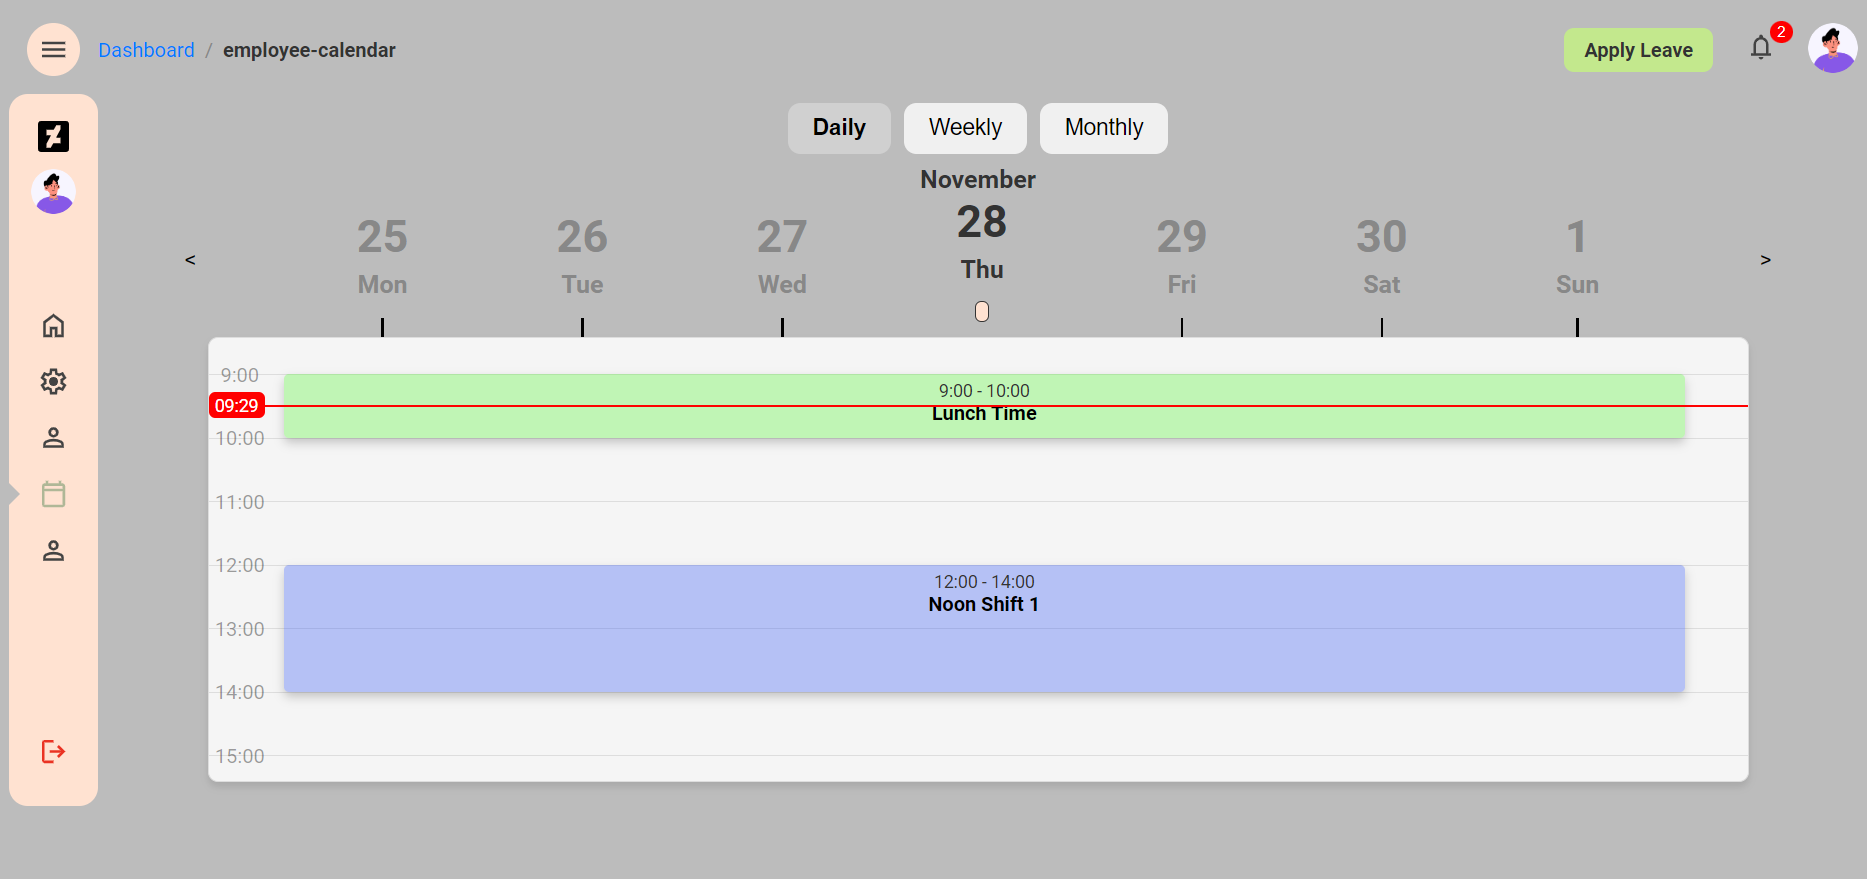
\includegraphics[width=0.8\columnwidth]{EmployeePages/DailySchedule.png}
    \caption{Daily Schedule}
    \label{fig:employee-daily-schedule}
    \end{figure}

    \begin{figure}[H]
    \centering
    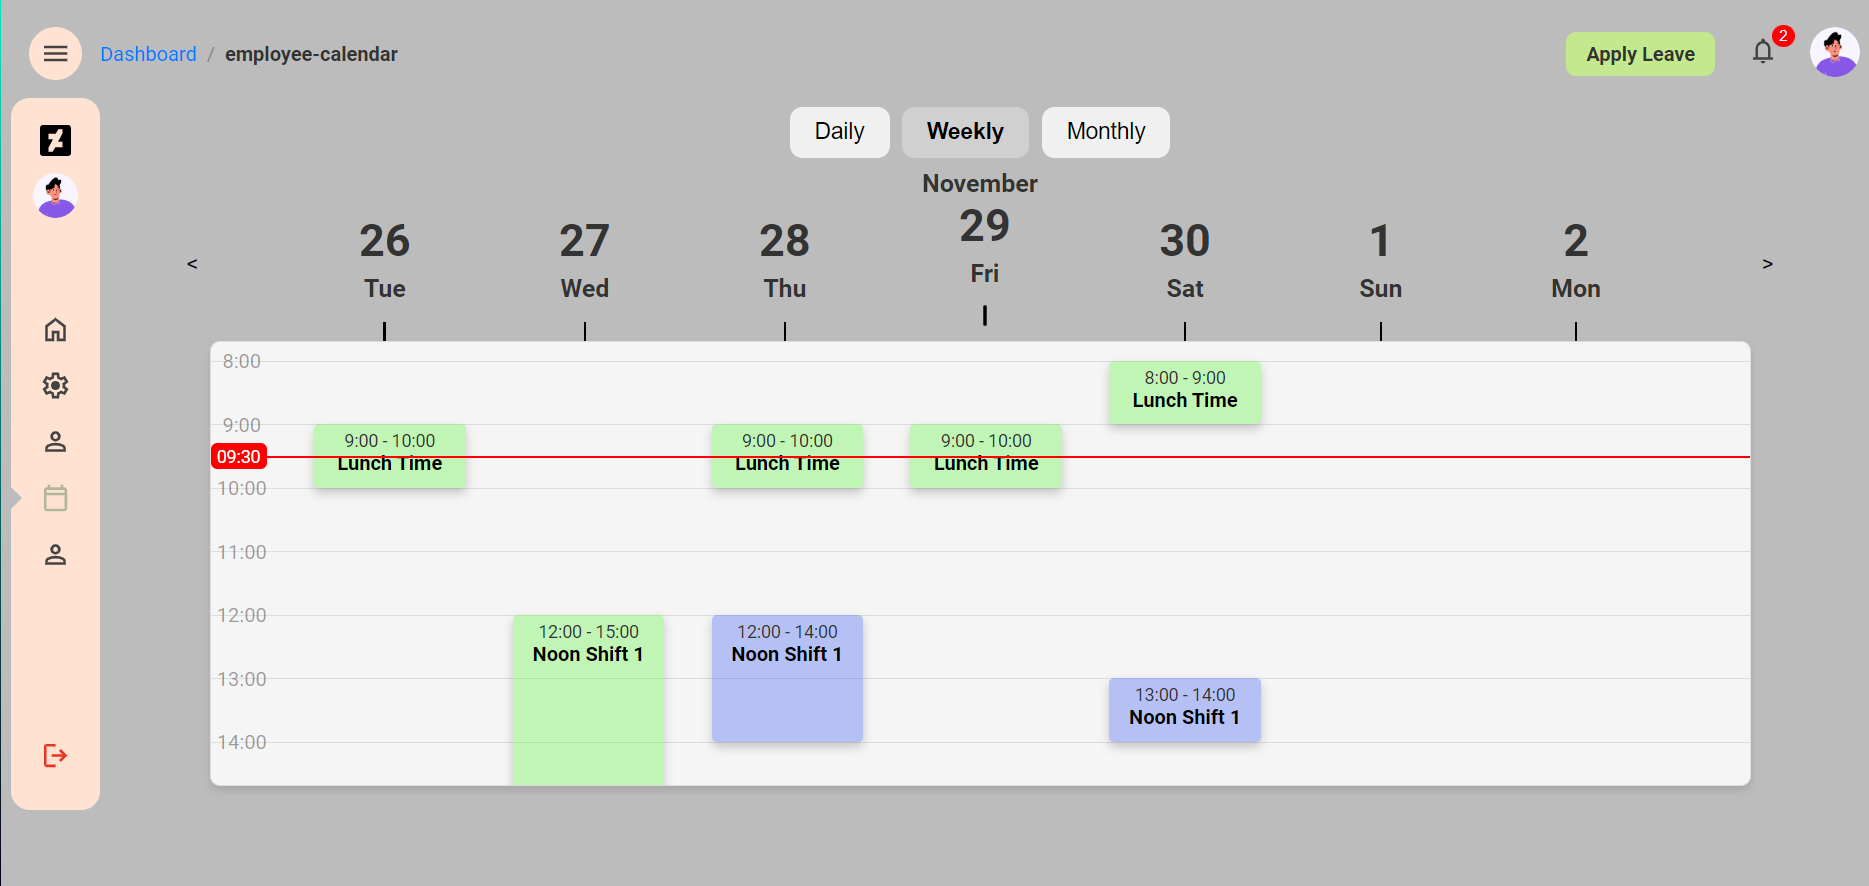
\includegraphics[width=0.8\columnwidth]{EmployeePages/WeeklySchedule.png}
    \caption{Weekly Schedule}
    \label{fig:employee-weekly-schedule}
    \end{figure}
    
    \begin{figure}[H]
    \centering
    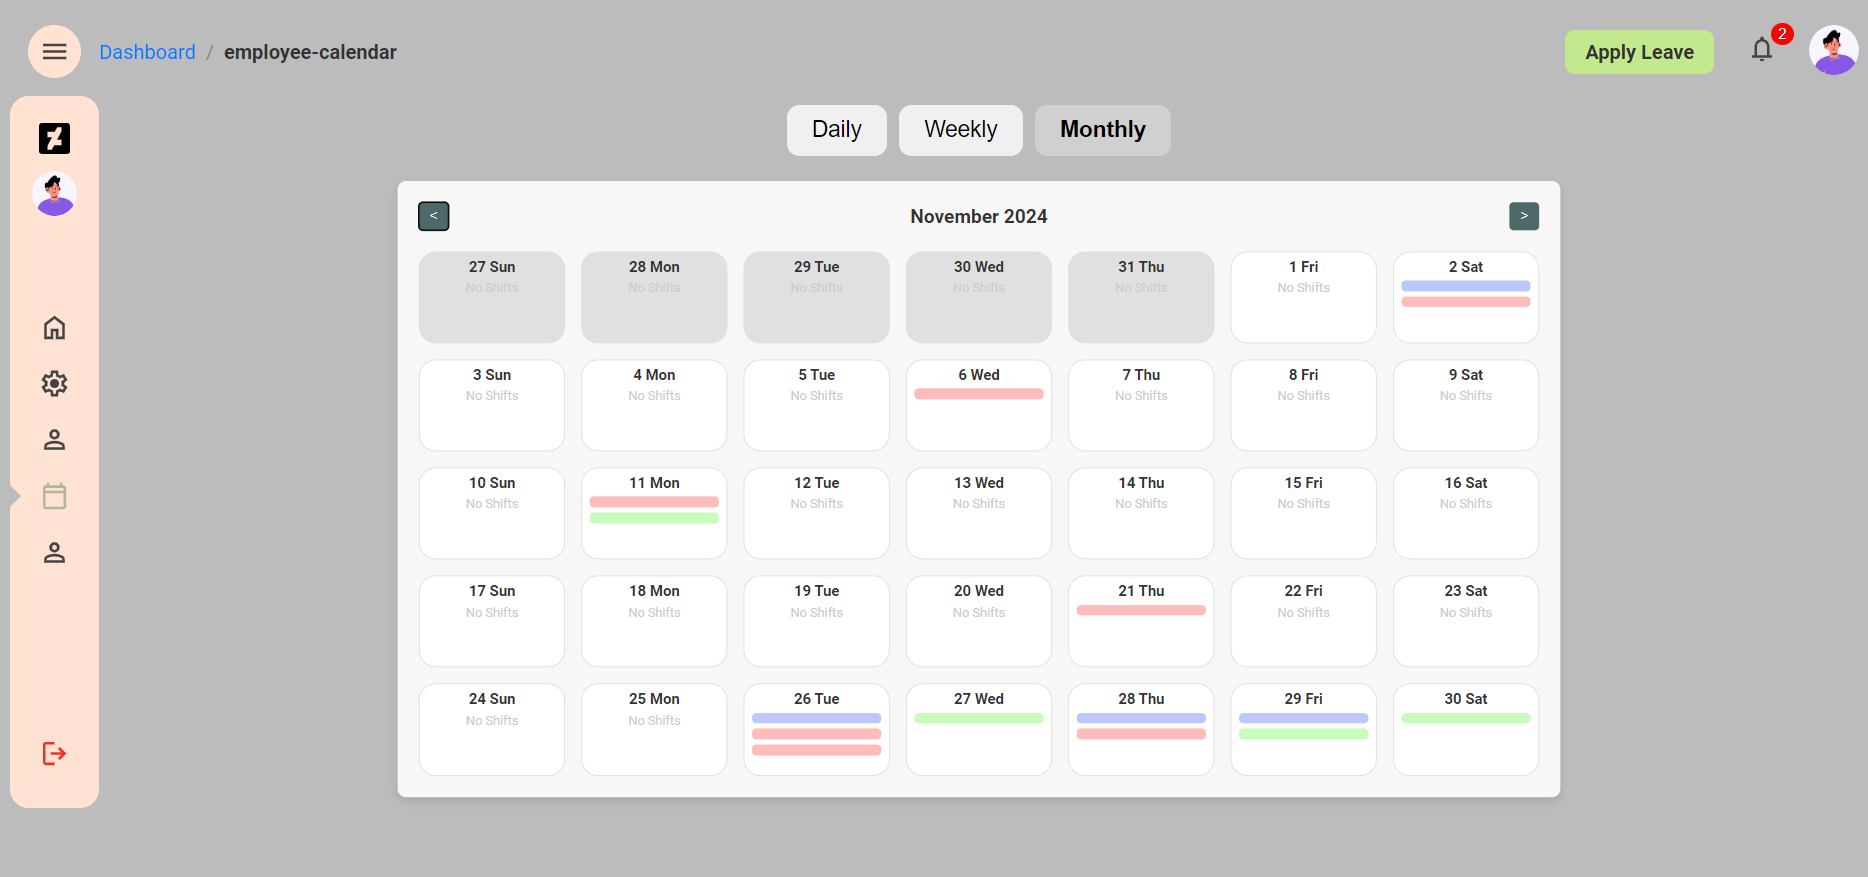
\includegraphics[width=0.8\columnwidth]{EmployeePages/MonthlySchedule.png}
    \caption{Monthly Schedule}
    \label{fig:employee-monthly-schedule}
    \end{figure}
    
    \item \textbf{Leave Request Submission:} Employees can submit leave requests by specifying the dates and reason in the leave request form.
    \begin{figure}[H]
    \centering
    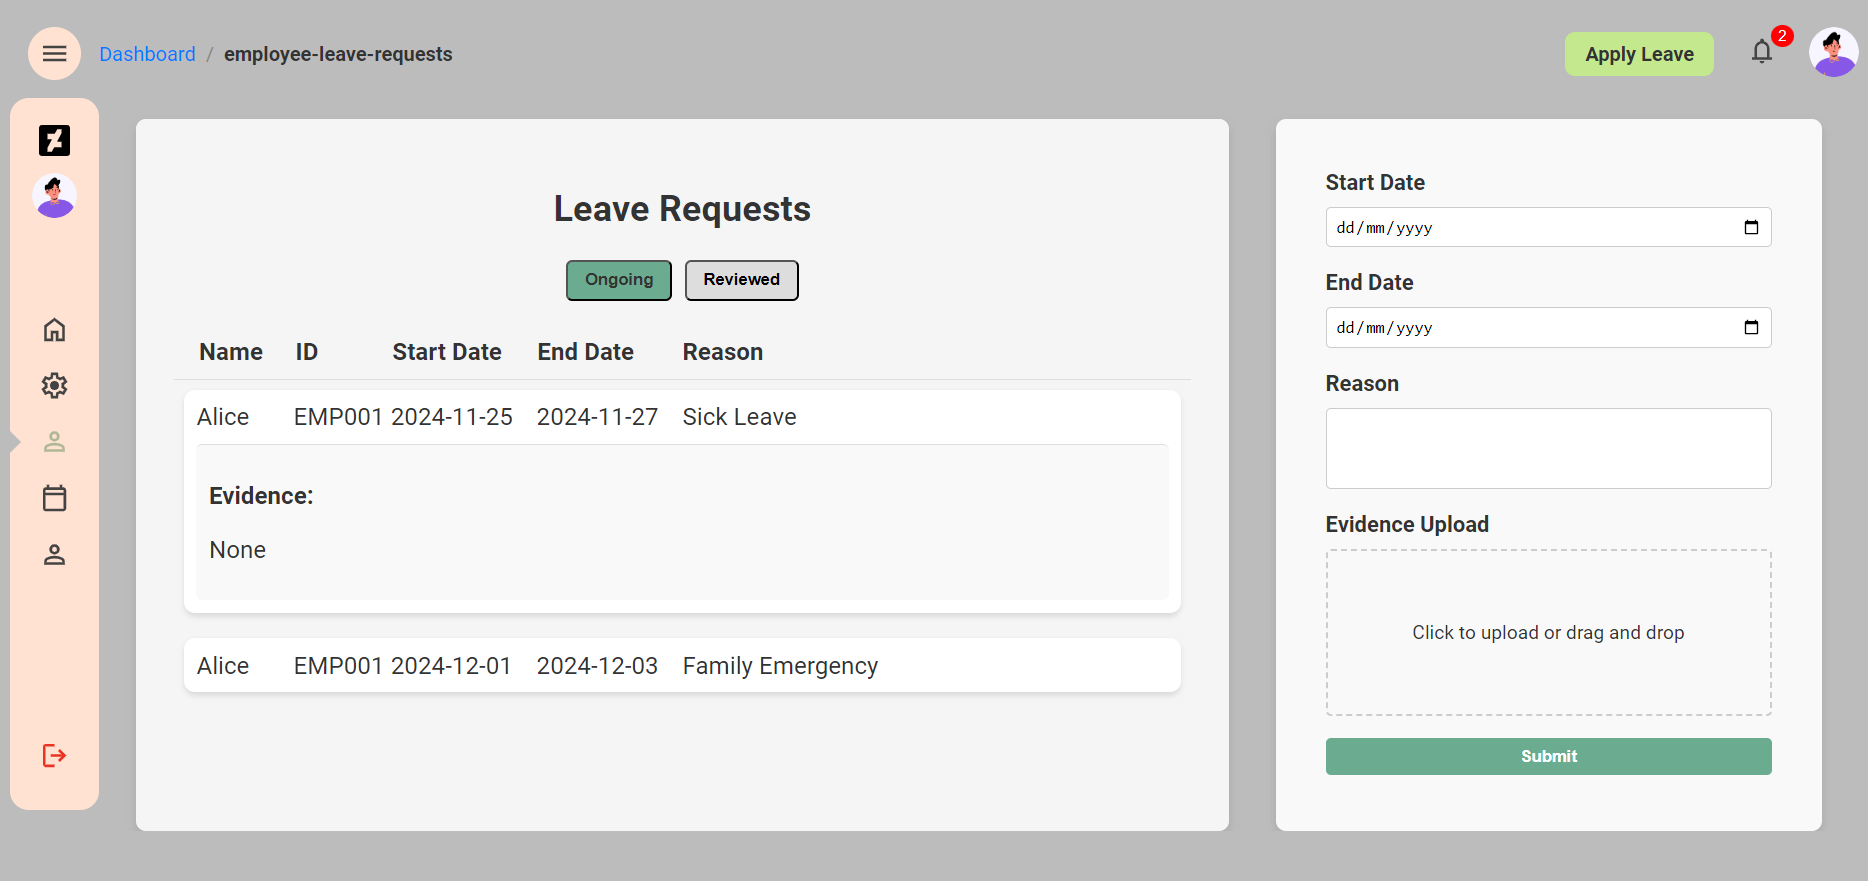
\includegraphics[width=0.8\columnwidth]{EmployeePages/LeaveRequest.png}
    \caption{Ongoing Leave Requests}
    \label{fig:employee-on-leave-request}
    \end{figure}

    \begin{figure}[H]
    \centering
    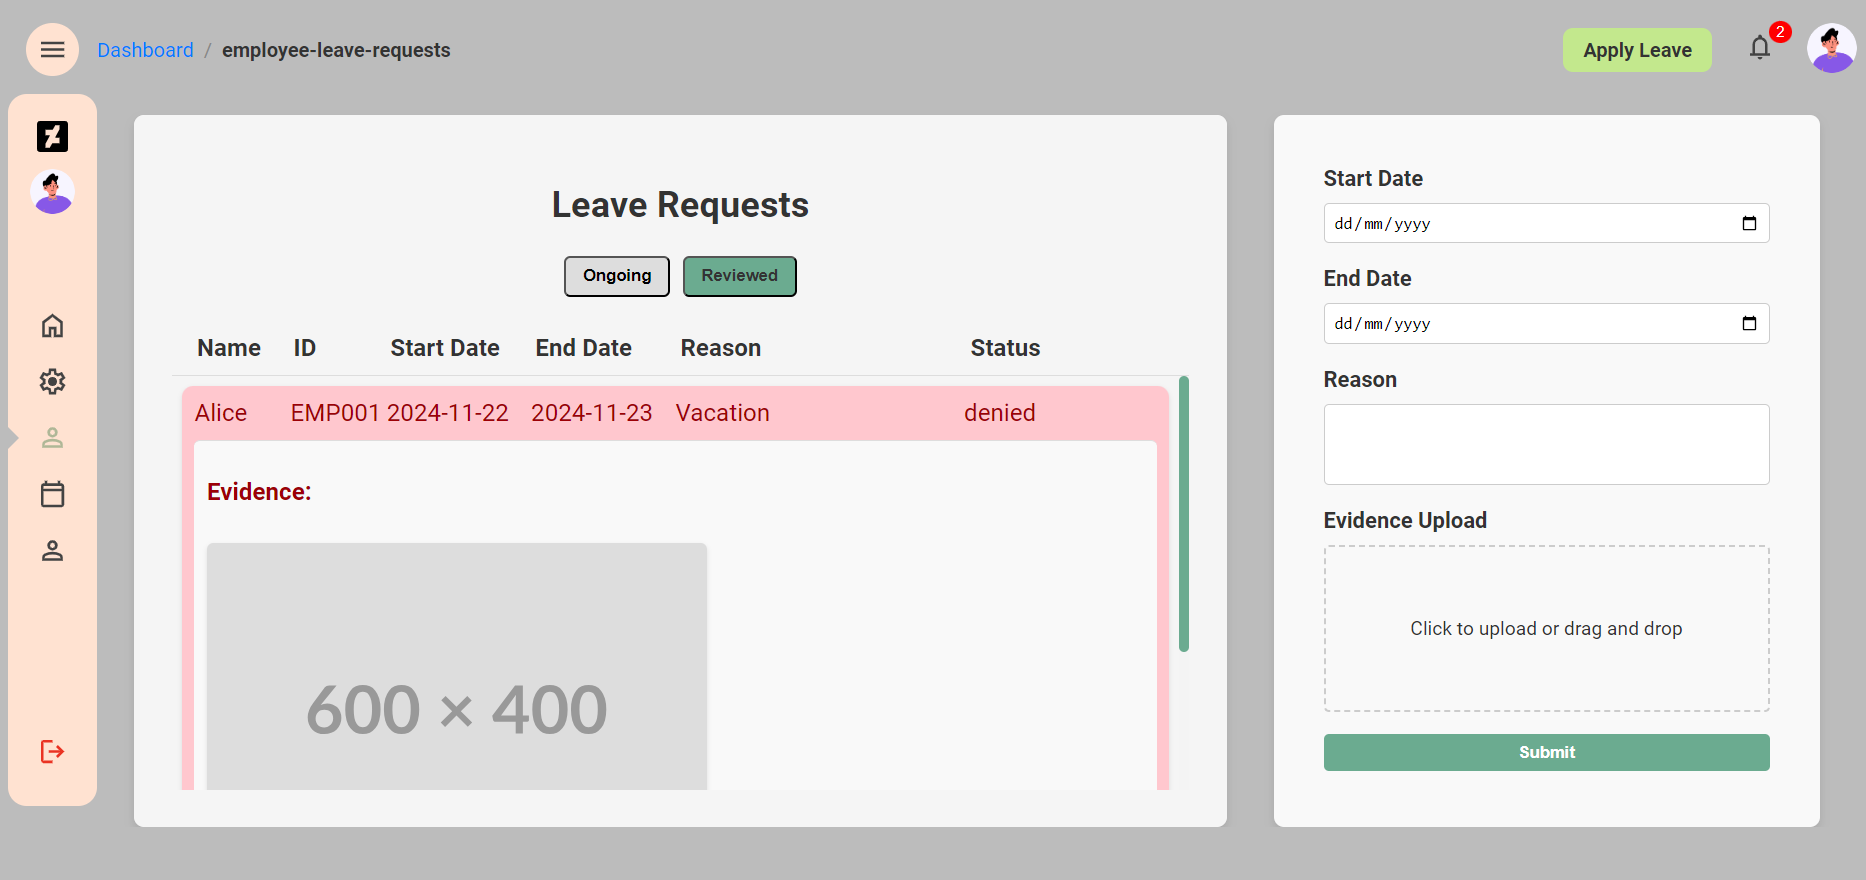
\includegraphics[width=0.8\columnwidth]{EmployeePages/LeaveRequest2.png}
    \caption{Reviewed Leave Requests}
    \label{fig:employee-rev-leave-request}
    \end{figure}
    
    \item \textbf{Export Data:} Employees can export their working data in the format they preferred. They are able to choose to separate files or compile into one file.
    
    \begin{figure}[H]
    \centering
    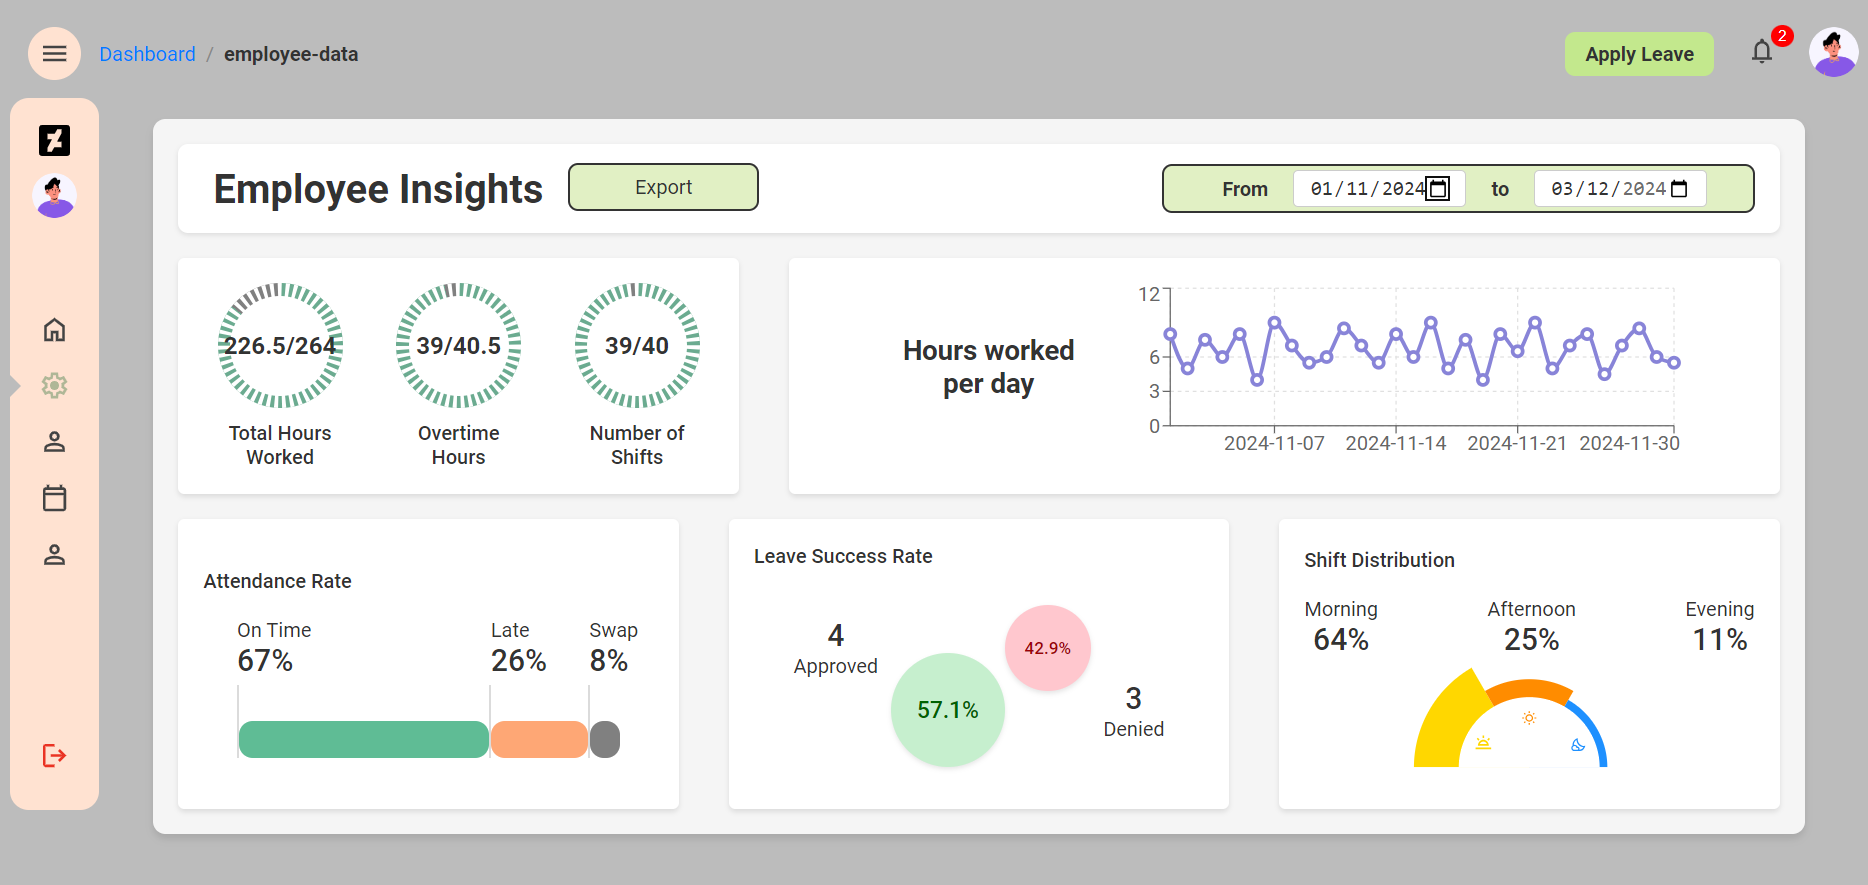
\includegraphics[width=0.8\columnwidth]{EmployeePages/ExportData3.png}
    \caption{Employee Insights Page}
    \label{fig:employee-insight-page}
    \end{figure}

    \begin{figure}[H]
    \centering
    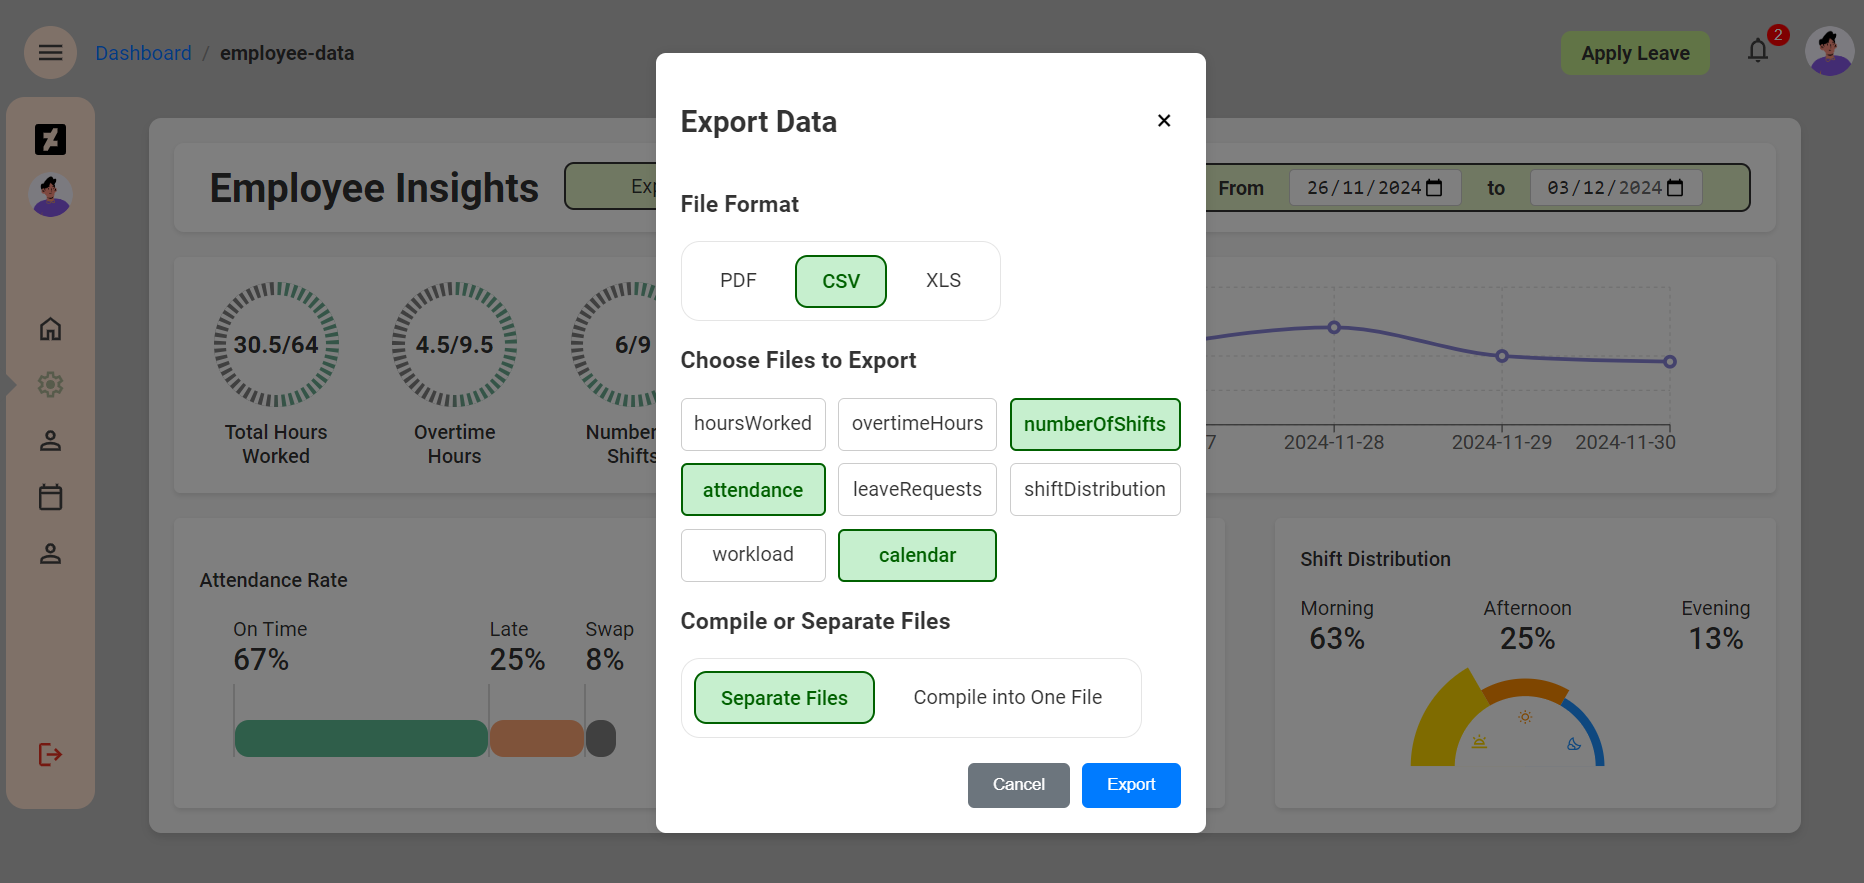
\includegraphics[width=0.8\columnwidth]{EmployeePages/ExportData2.png}
    \caption{Export Data Form}
    \label{fig:employee-export-data}
    \end{figure}

    \item \textbf{Edit Profile:} Employee can view their personal details, working preference and weekly overview. Additionally,they edit their personal information, preferred shift time, minimum rest periods, day off and shift swap preferences.
    
    \begin{figure}[H]
    \centering
    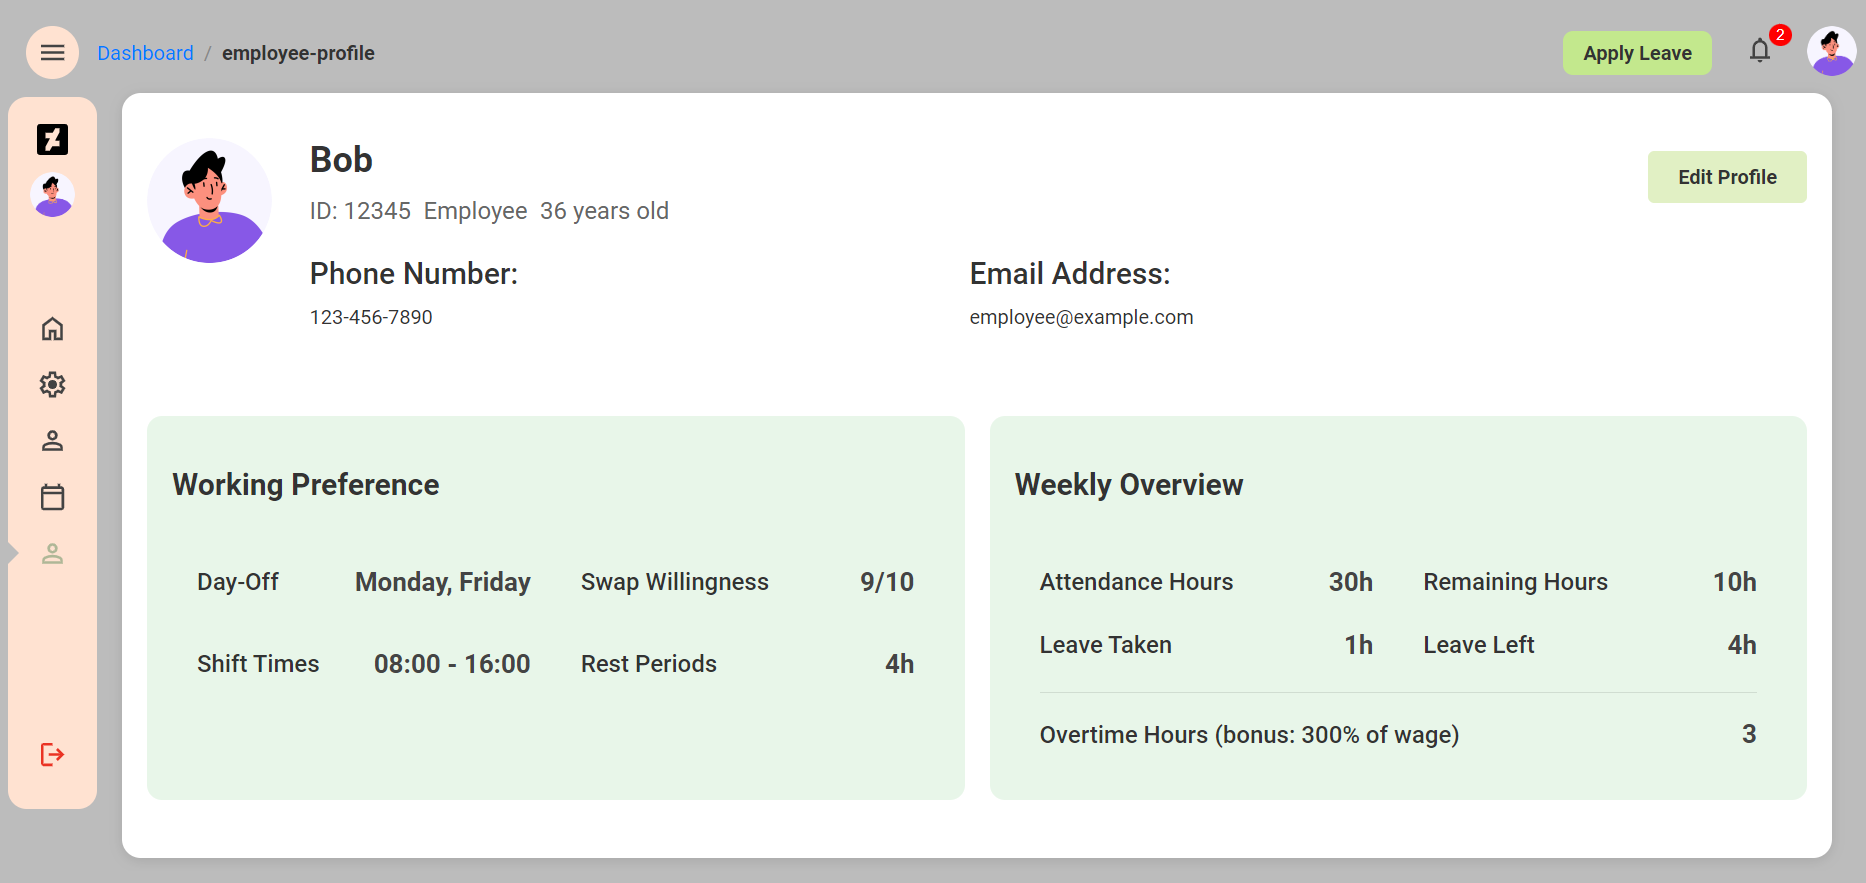
\includegraphics[width=0.8\columnwidth]{EmployeePages/EditProfile.png}
    \caption{Edit Profile Page}
    \label{fig:employee-profile}
    \end{figure}

    \begin{figure}[H]
    \centering
    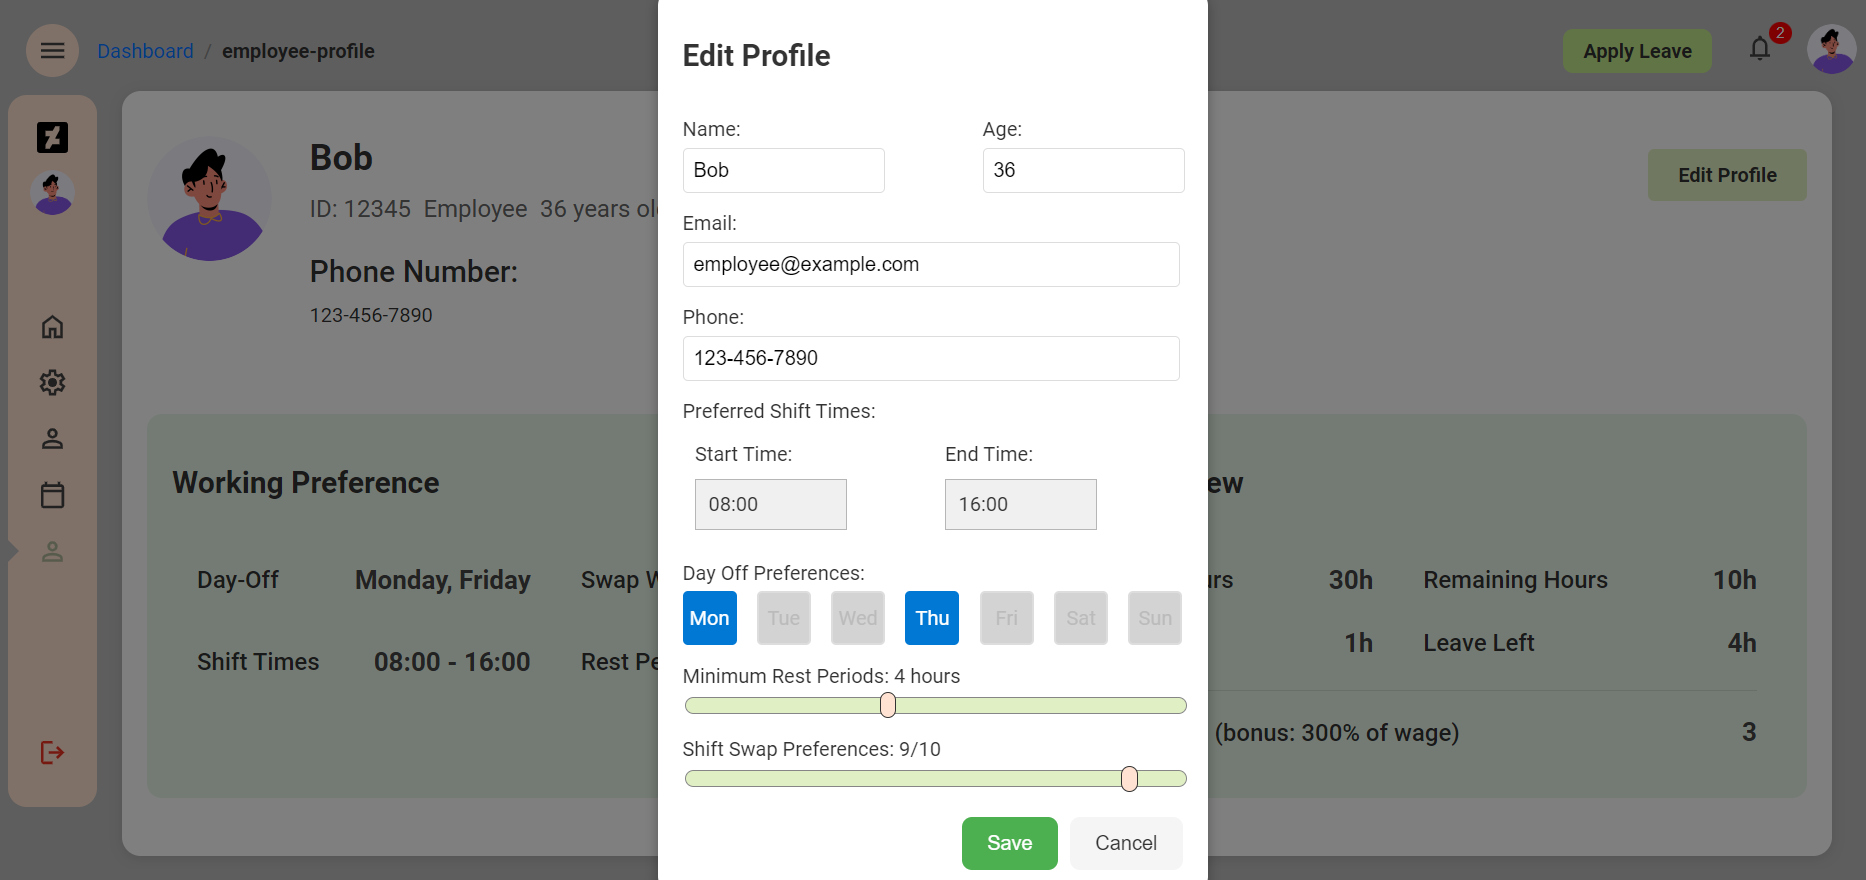
\includegraphics[width=0.8\columnwidth]{EmployeePages/EditProfile2.png}
    \caption{Edit Profile Form}
    \label{fig:employee-edit-profile-form}
    \end{figure}

    \end{itemize}
    
\subsubsection{Manager Features}
\label{subsubsec:ManagerFeatures}
\begin{itemize}

    \item \textbf{View Calendar:} Manager are able to view a calendar detailed with employee leaves and holidays.

    \begin{figure}[H]
        \centering
        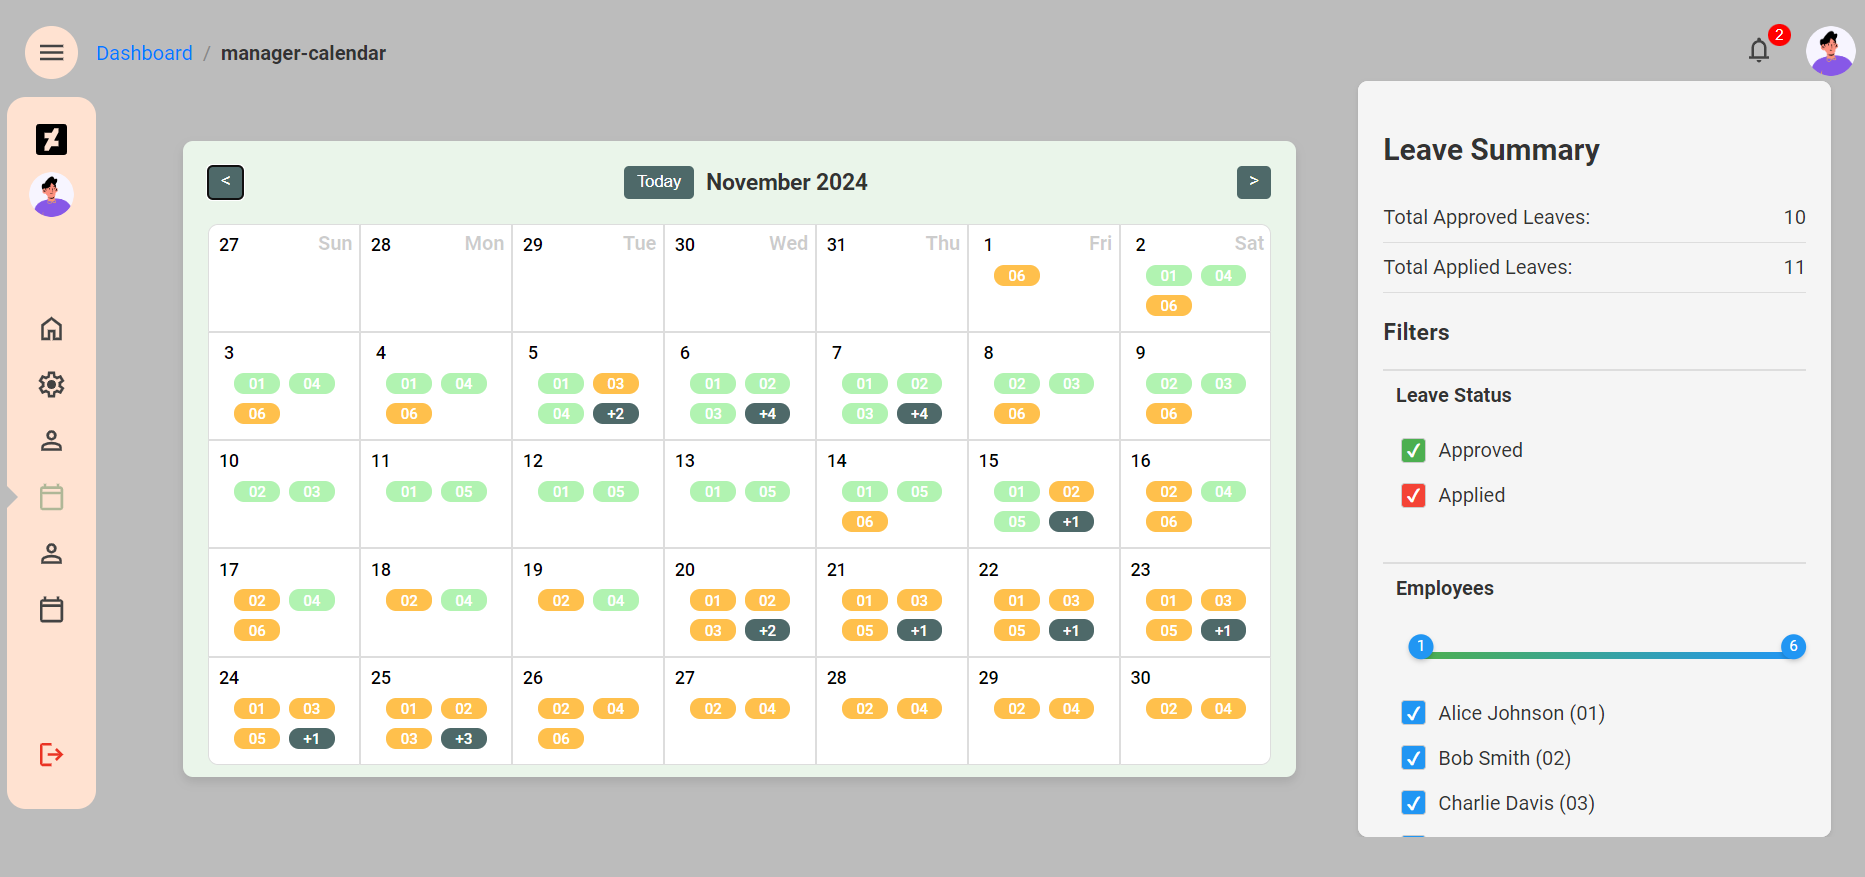
\includegraphics[width=0.8\linewidth]{ManagerPages/ManagerCalendar.png}
        \caption{Manager Calendar}
        \label{fig:manager-calendar}
    \end{figure}
    \begin{figure}[H]
        \centering
        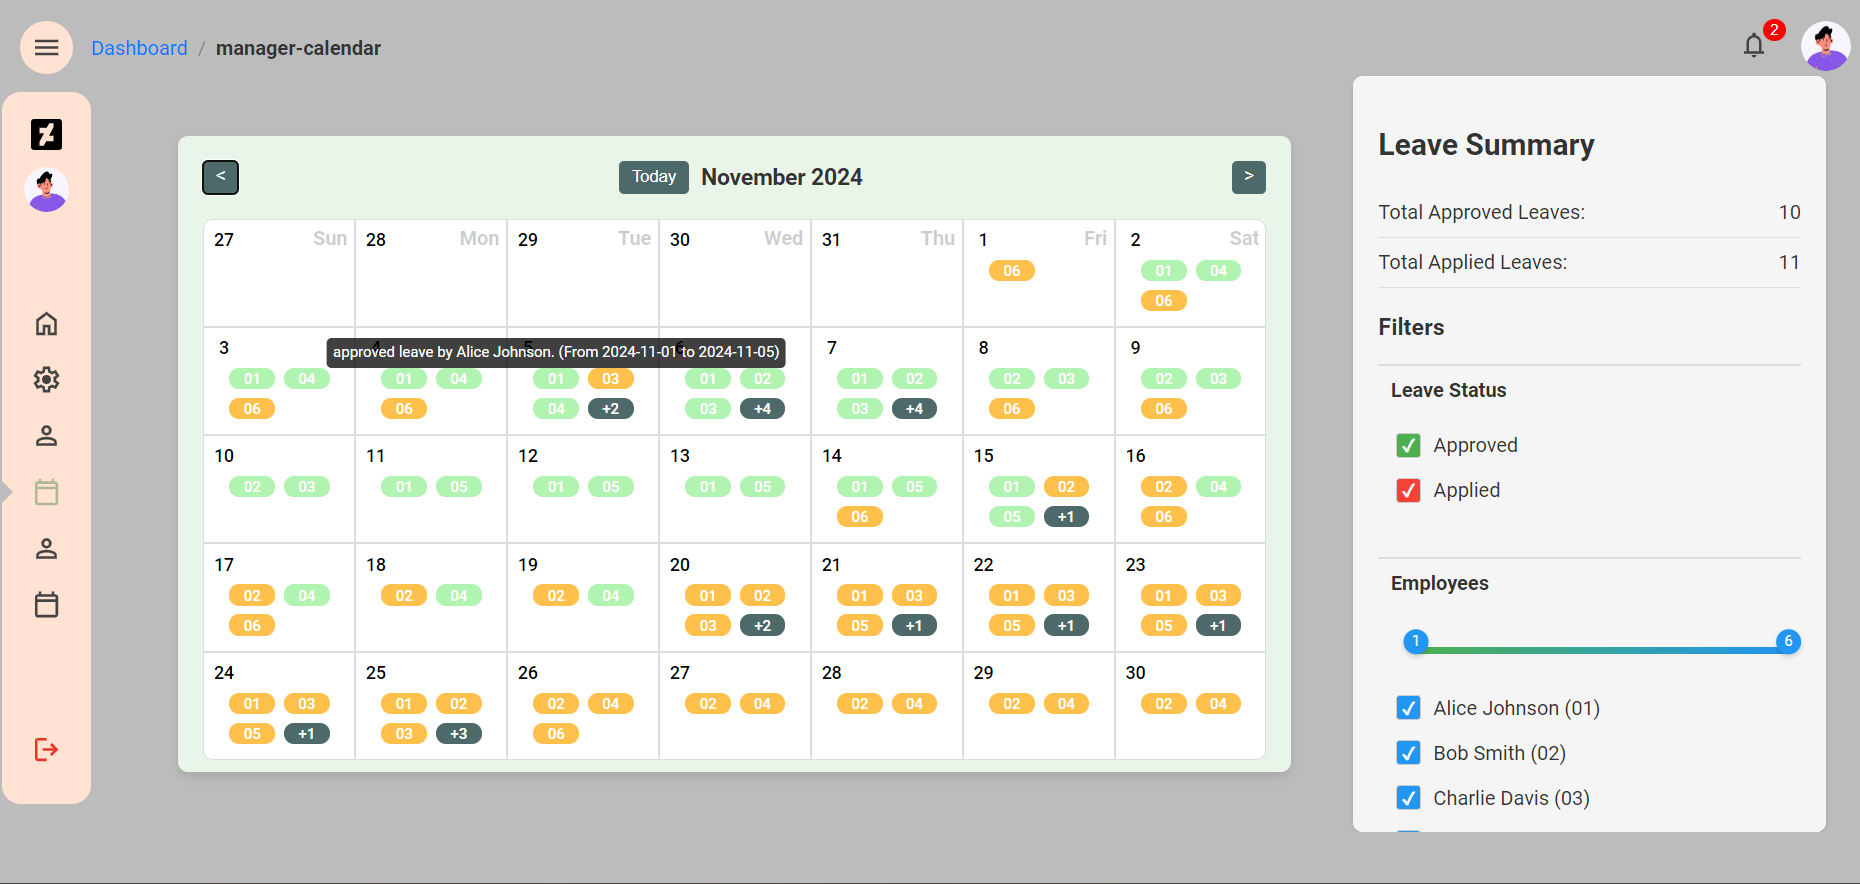
\includegraphics[width=0.8\linewidth]{ManagerPages/ManagerCalendar2.png}
        \caption{Manager Calendar Hover}
        \label{fig:manager-calendar-h}
    \end{figure}
    
    \item \textbf{Review Leave Request:} Manager are able to approve or deny employee's leave requests.

    \begin{figure}[H]
    \centering
    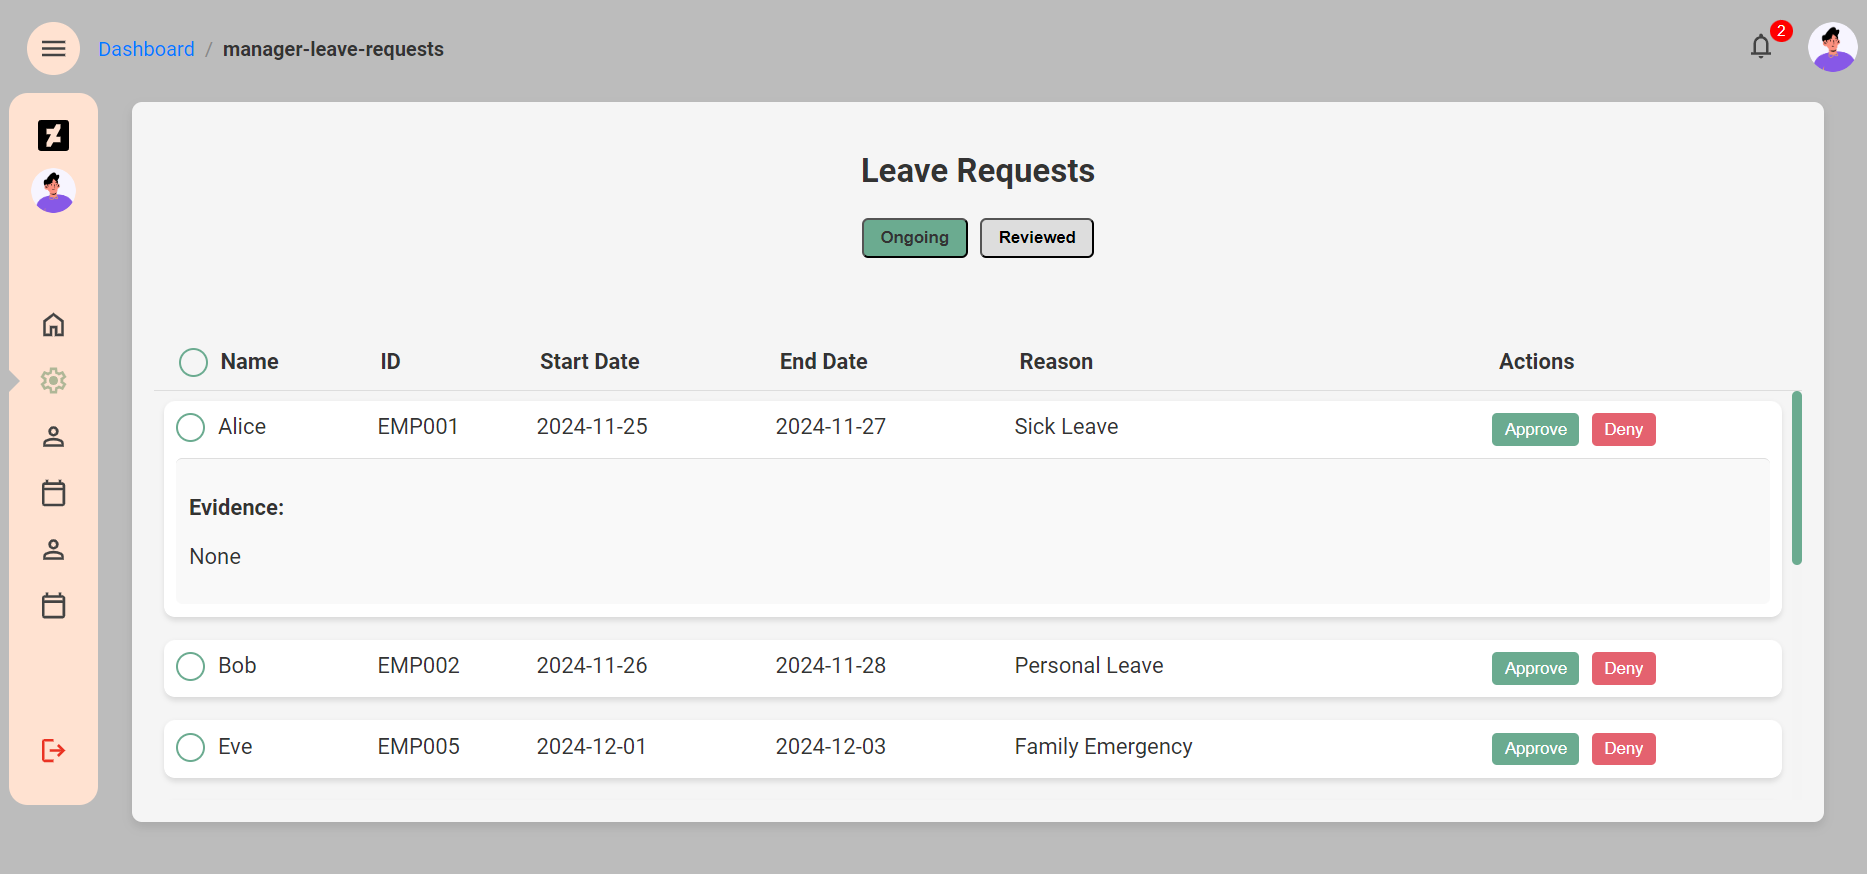
\includegraphics[width=0.8\columnwidth]{ManagerPages/ManagerLeaveRequest.png}
    \caption{Manager Ongoing Leave Requests}
    \label{fig:manager-on-leave-request}
    \end{figure}

    \begin{figure}[H]
    \centering
    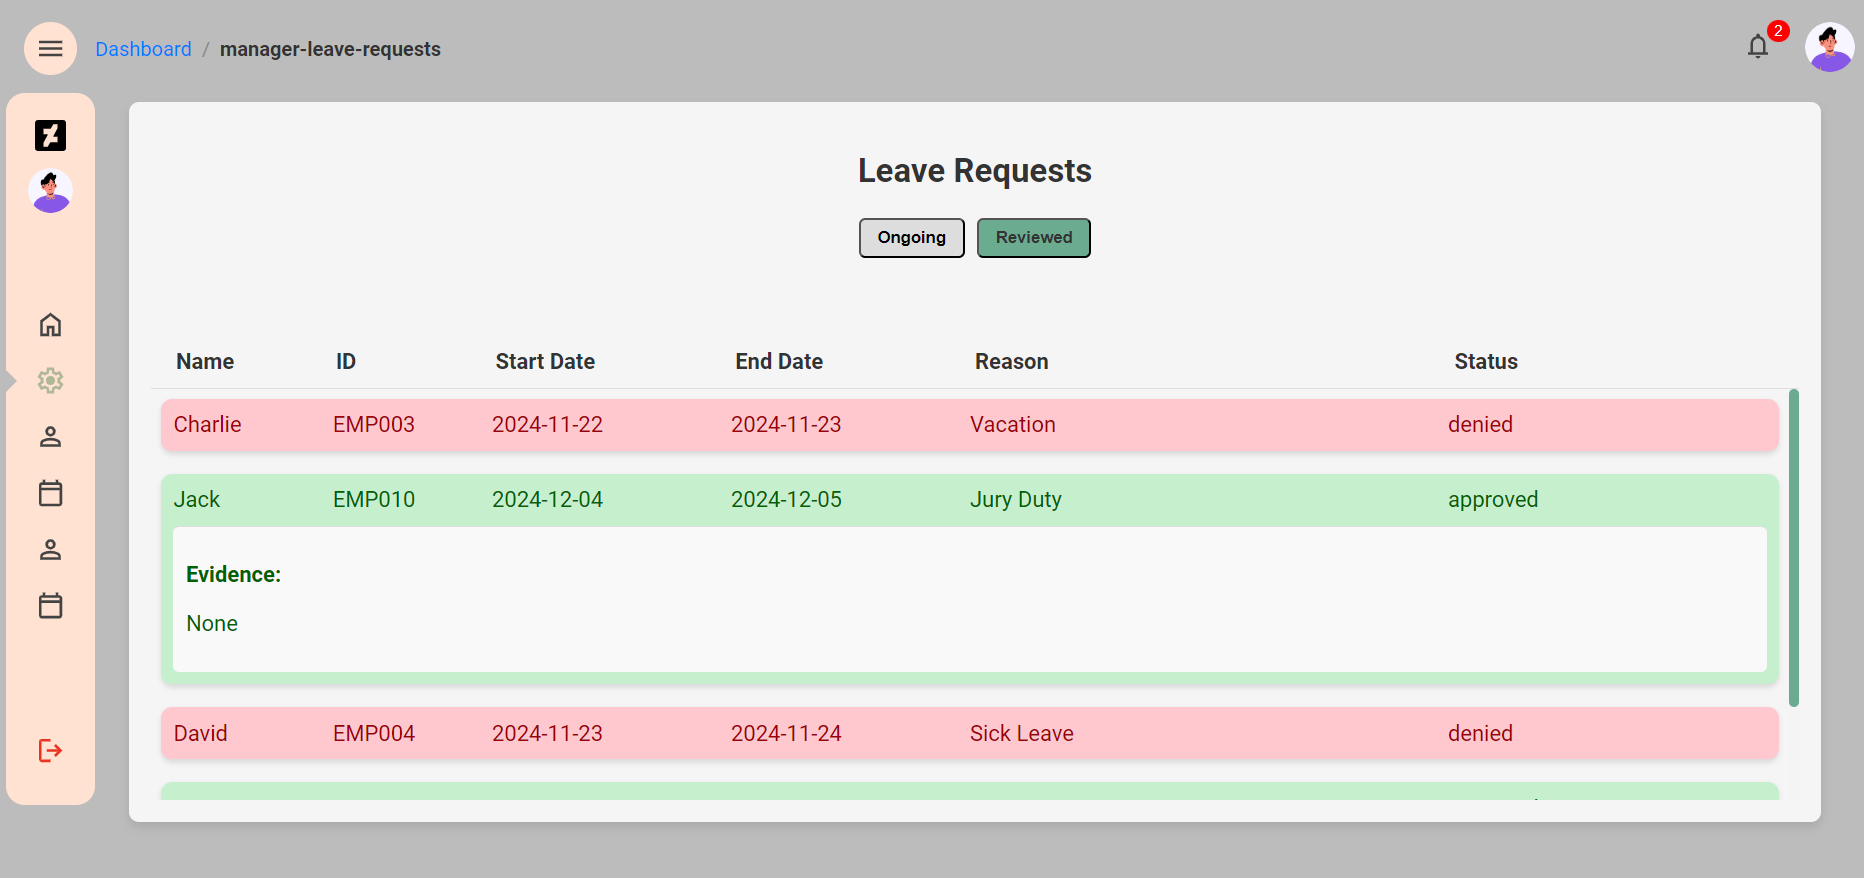
\includegraphics[width=0.8\columnwidth]{ManagerPages/ManagerLeaveRequest2.png}
    \caption{Manager Reviewed Leave Requests}
    \label{fig:manager-rev-leave-request}
    \end{figure}

    
    \item \textbf{Schedule Management:} Managers can view employee's schedules from a day to seven days. Manager can swap employee's shifts.

    \begin{figure}[H]
    \centering
    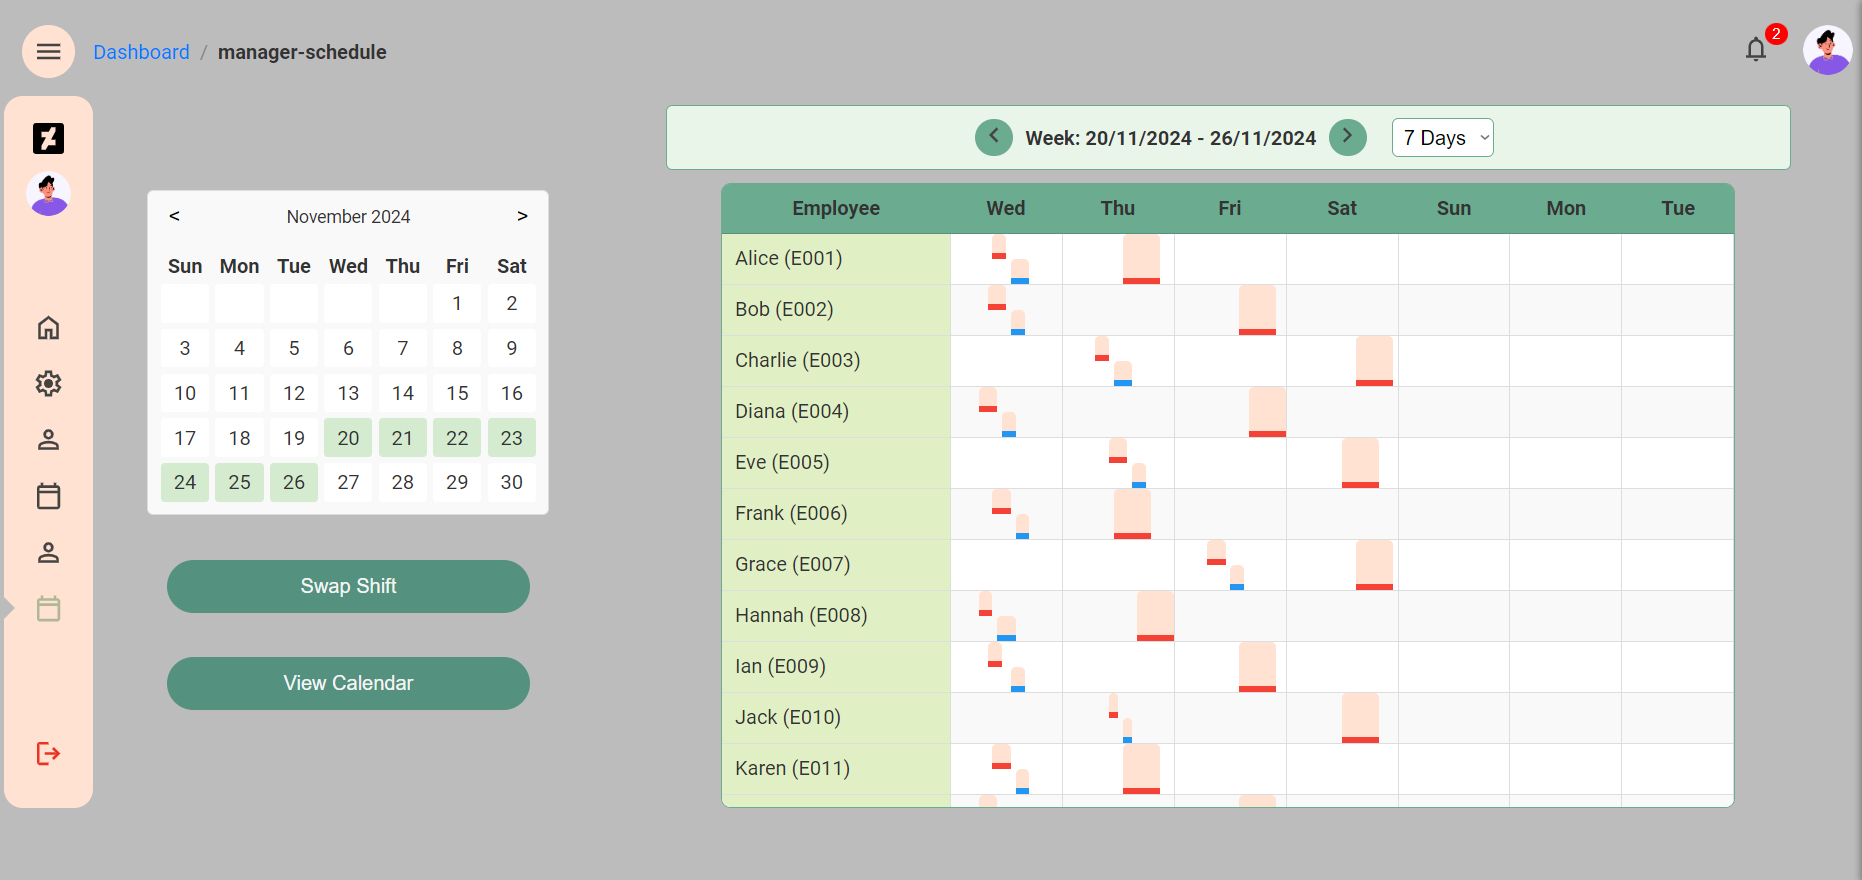
\includegraphics[width=0.8\columnwidth]{ManagerPages/ManagerSchedule.png}
    \caption{Manager Schedule Page}
    \label{fig:manager-schedule}
    \end{figure}

    \begin{figure}[H]
    \centering
    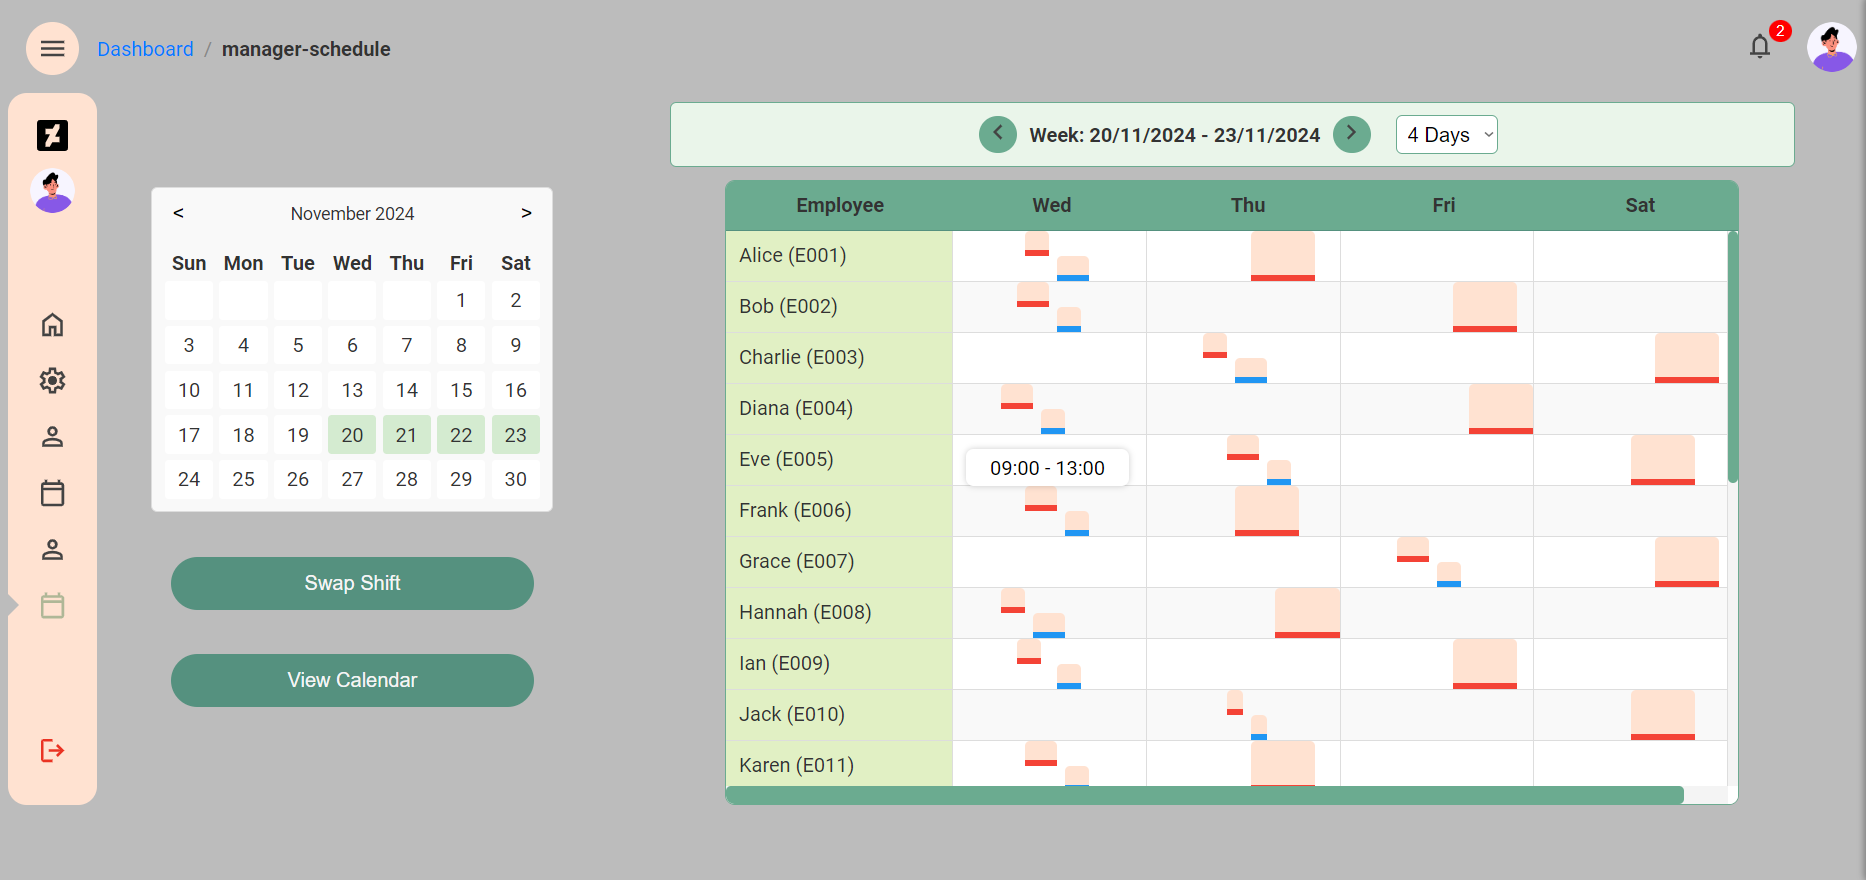
\includegraphics[width=0.8\columnwidth]{ManagerPages/ManagerSchedule2.png}
    \caption{Manager Schedule Page 4 Days View}
    \label{fig:manager-schedule-4}
    \end{figure}

    \begin{figure}[H]
    \centering
    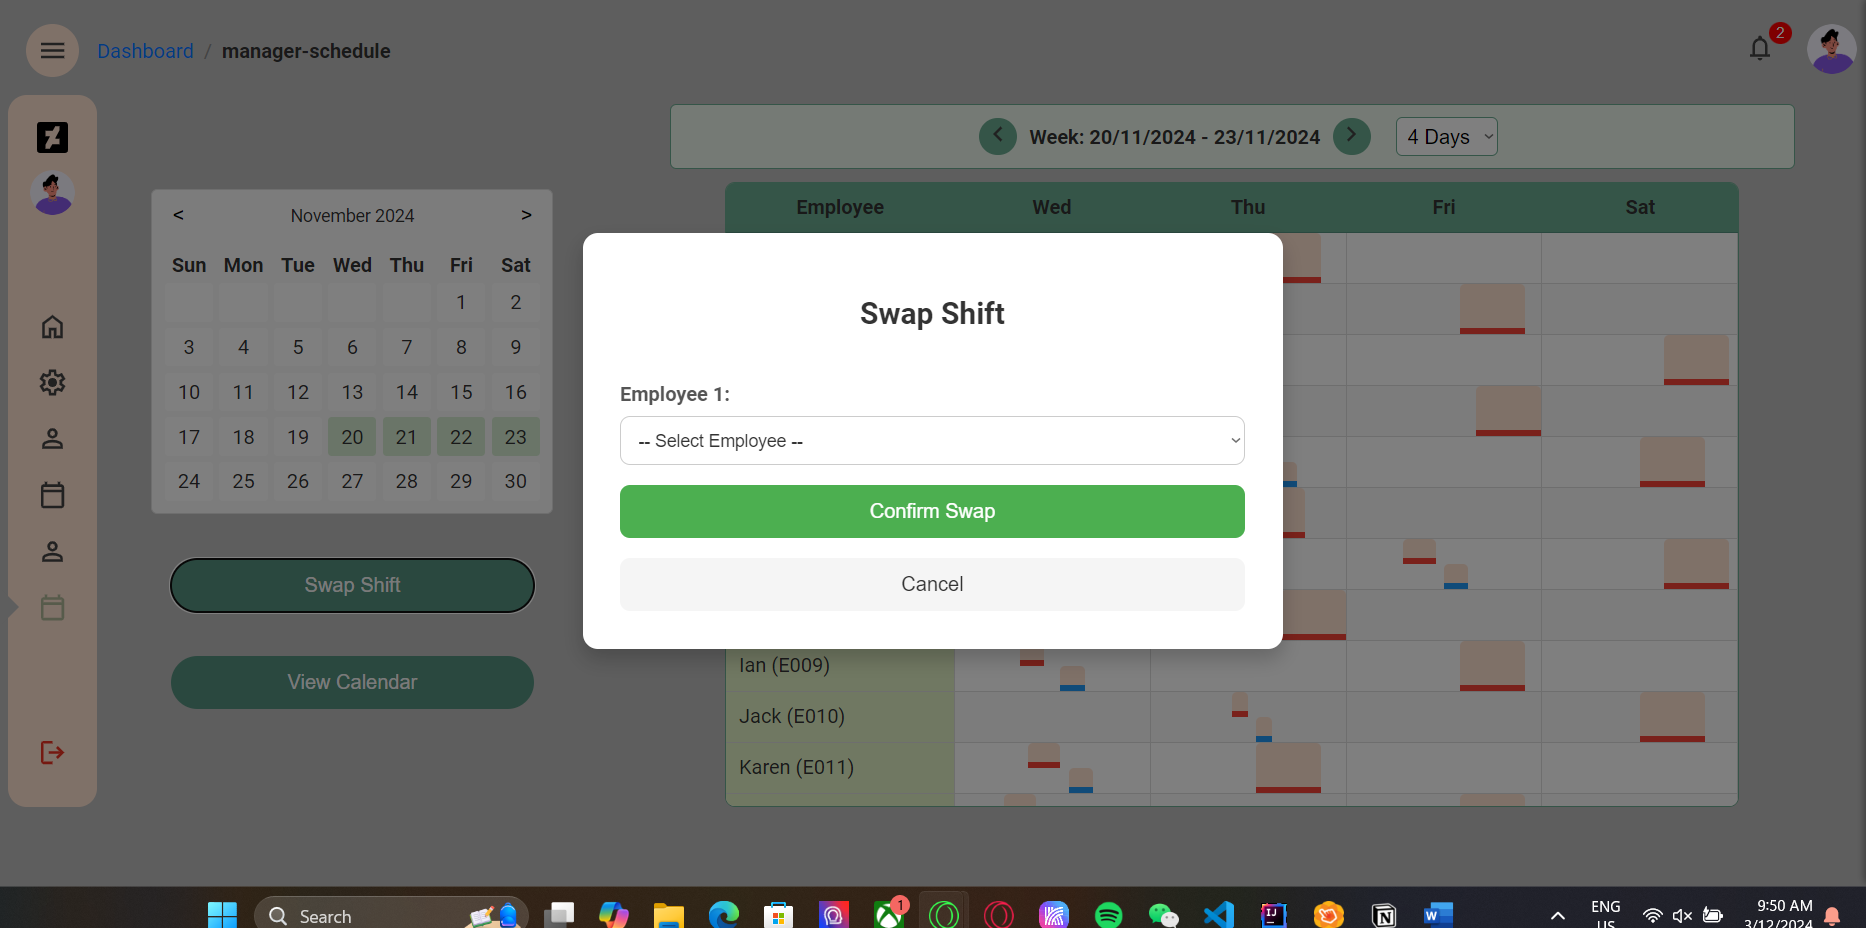
\includegraphics[width=0.8\columnwidth]{ManagerPages/ManagerSchedule3.png}
    \caption{Manager Shift Swap Form Collapsed}
    \label{fig:manager-shift-swap-form-c}
    \end{figure}

    \begin{figure}[H]
    \centering
    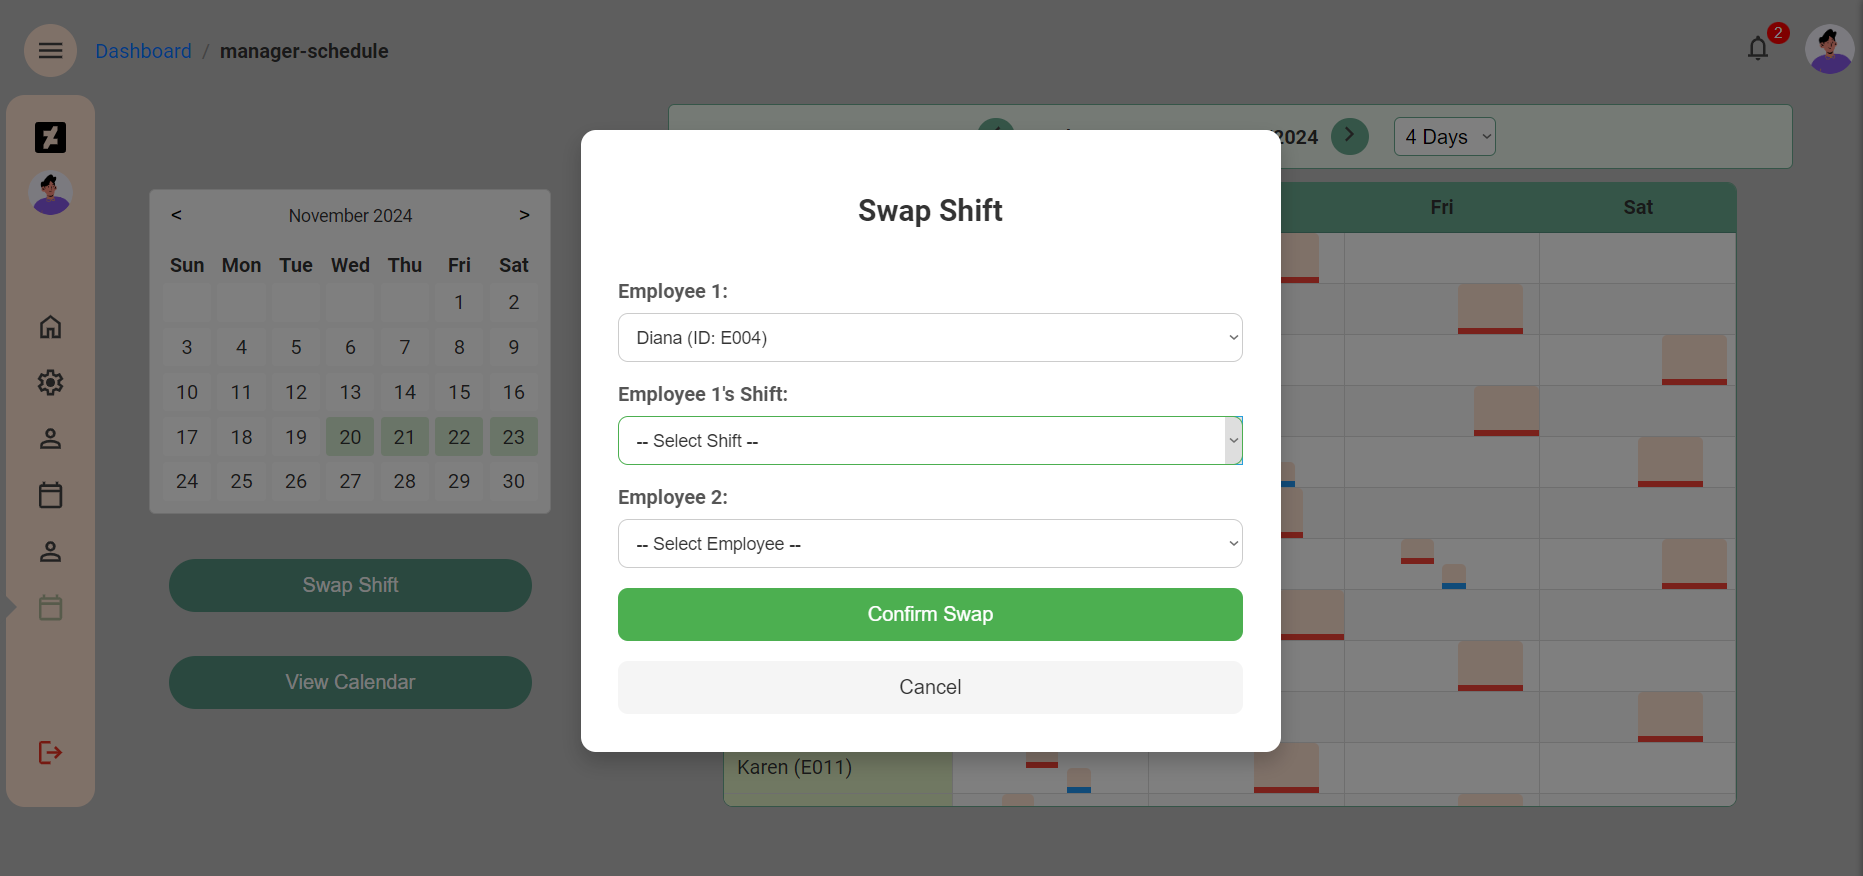
\includegraphics[width=0.8\columnwidth]{ManagerPages/ManagerSchedule4.png}
    \caption{Manager Shift Swap Form Expanded}
    \label{fig:manager-shift-swap-form-e}
    \end{figure}

    \begin{figure}[H]
    \centering
    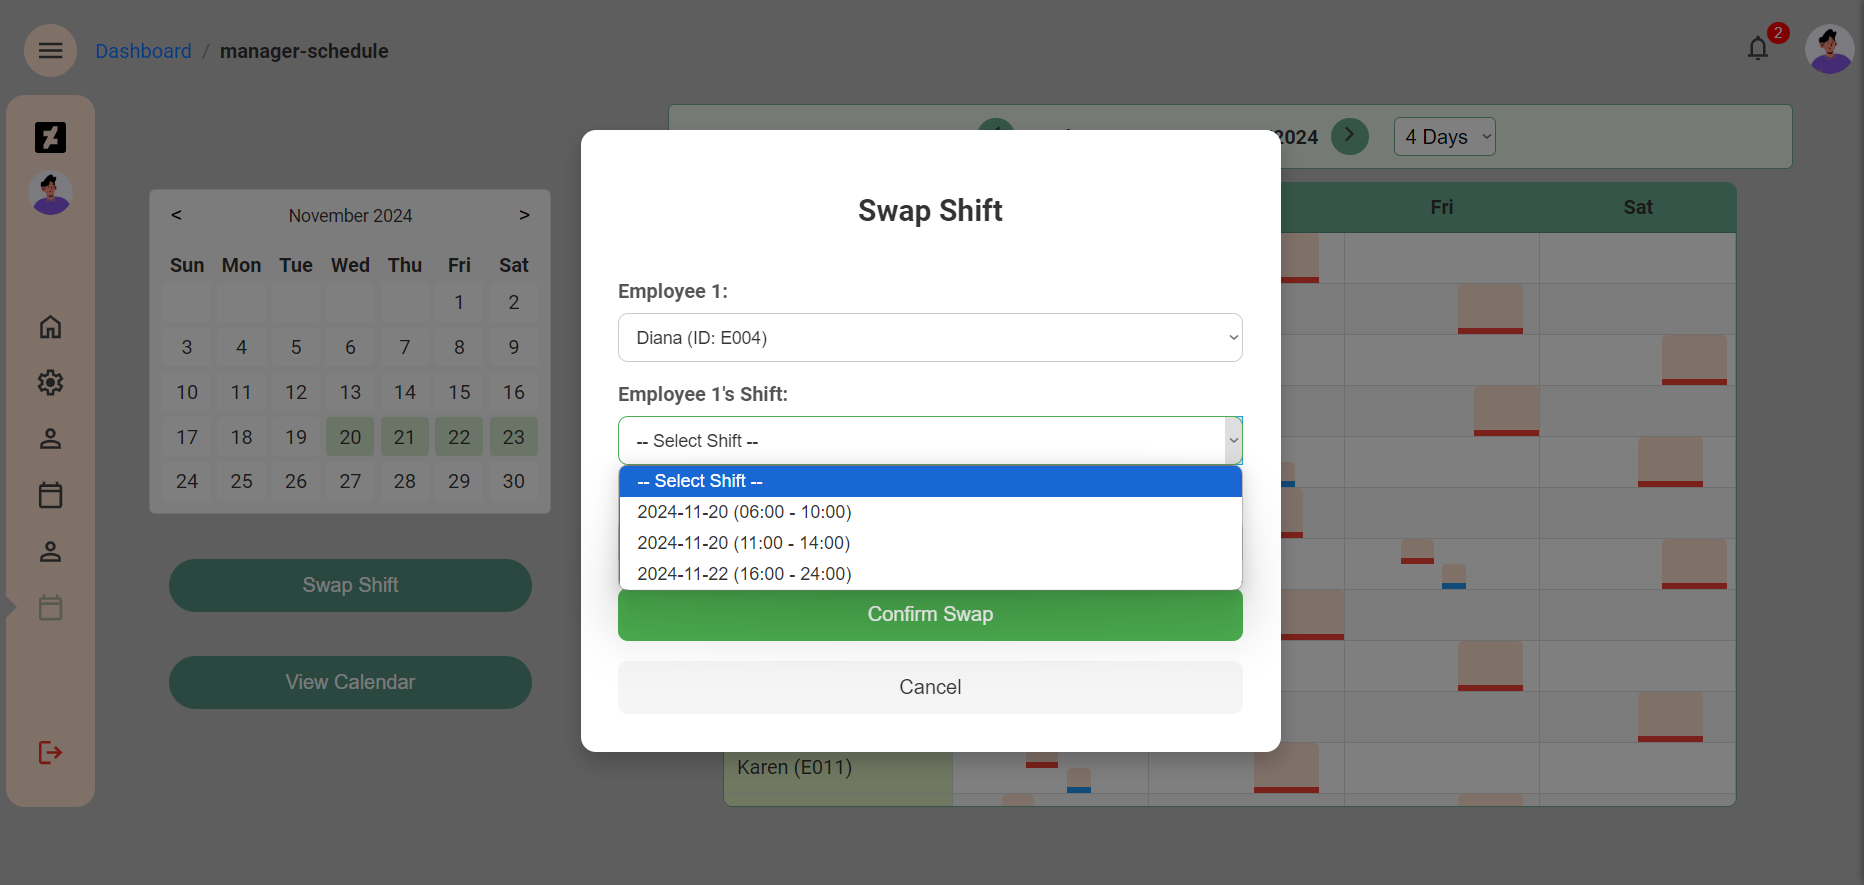
\includegraphics[width=0.8\columnwidth]{ManagerPages/ManagerSchedule5.png}
    \caption{Manager Shift Swap Form Expanded 2}
    \label{fig:manager-shift-swap-form-e-2}
    \end{figure}

    \begin{figure}[H]
    \centering
    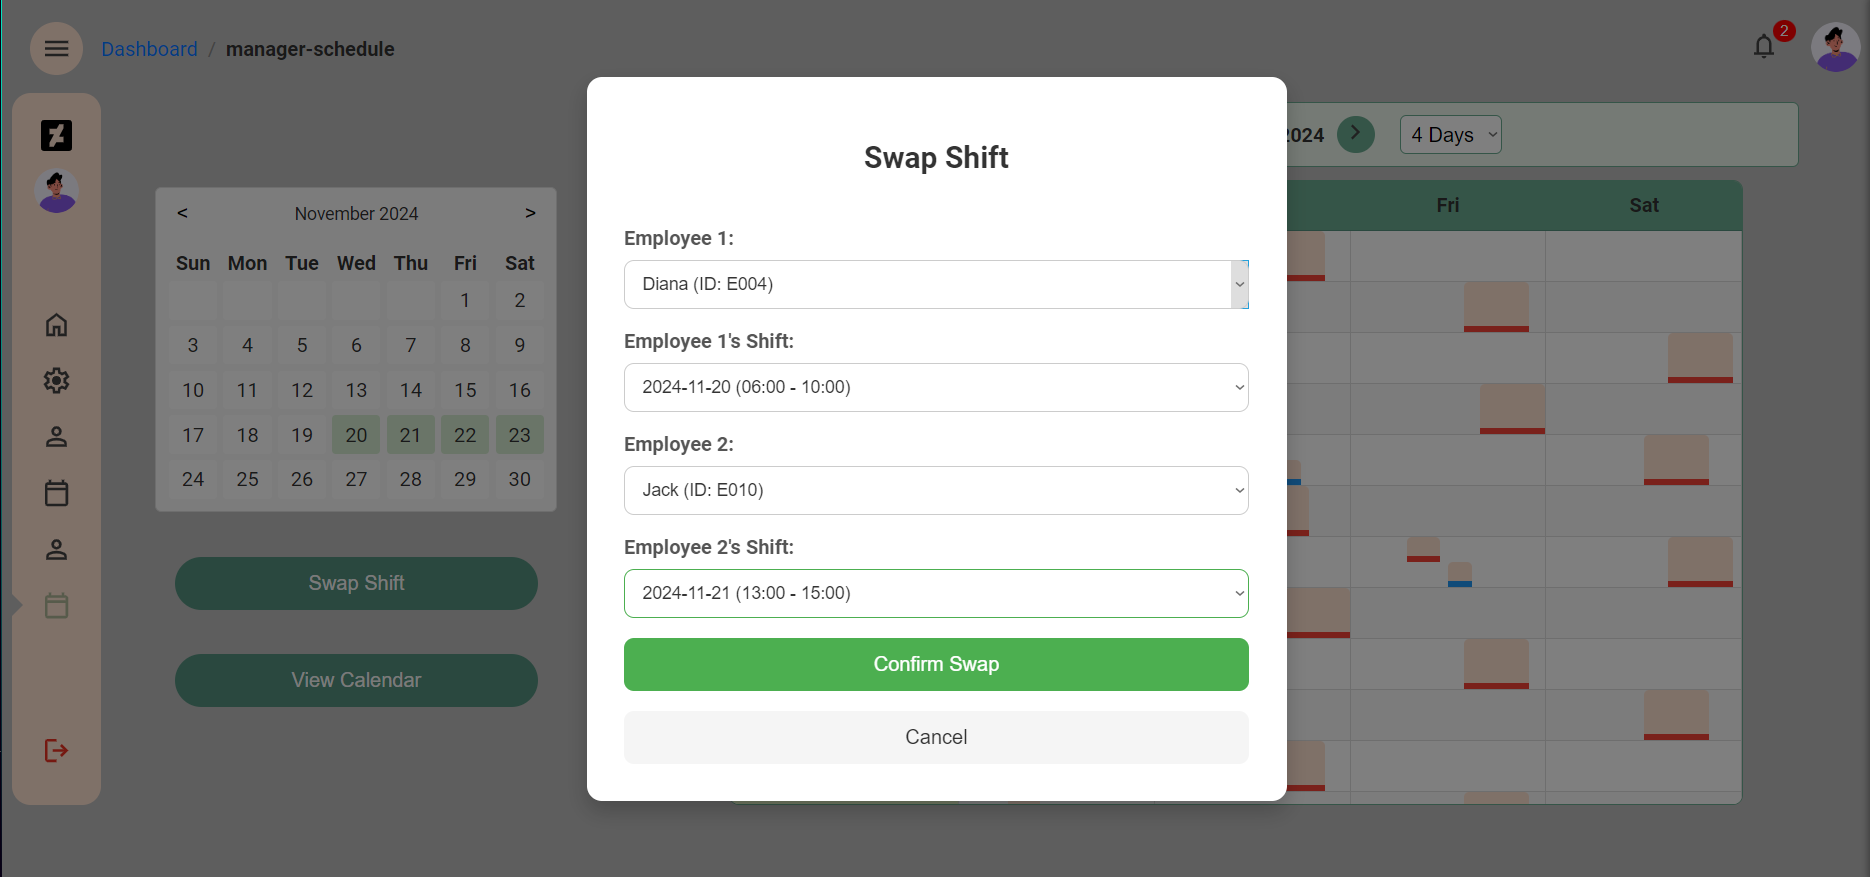
\includegraphics[width=0.8\columnwidth]{ManagerPages/ManagerSchedule6.png}
    \caption{Manager Shift Swap Form Expanded 3}
    \label{fig:manager-shift-swap-form-e-3}
    \end{figure}
    
    \item \textbf{Import/Export Data:} Manager can choose to import or export employee data, calendar data, rules data and schedule data. For employee data as shown in Figure \ref{fig:manager-employee-data-personal}, FIgure \ref{fig:manager-employee-data-attendance}, Figure 
    \ref{fig:manager-employee-data-preferences} we can export employee personal data, attendance records and also their shifts preferences.
    
     \begin{figure}[H]
    \centering
    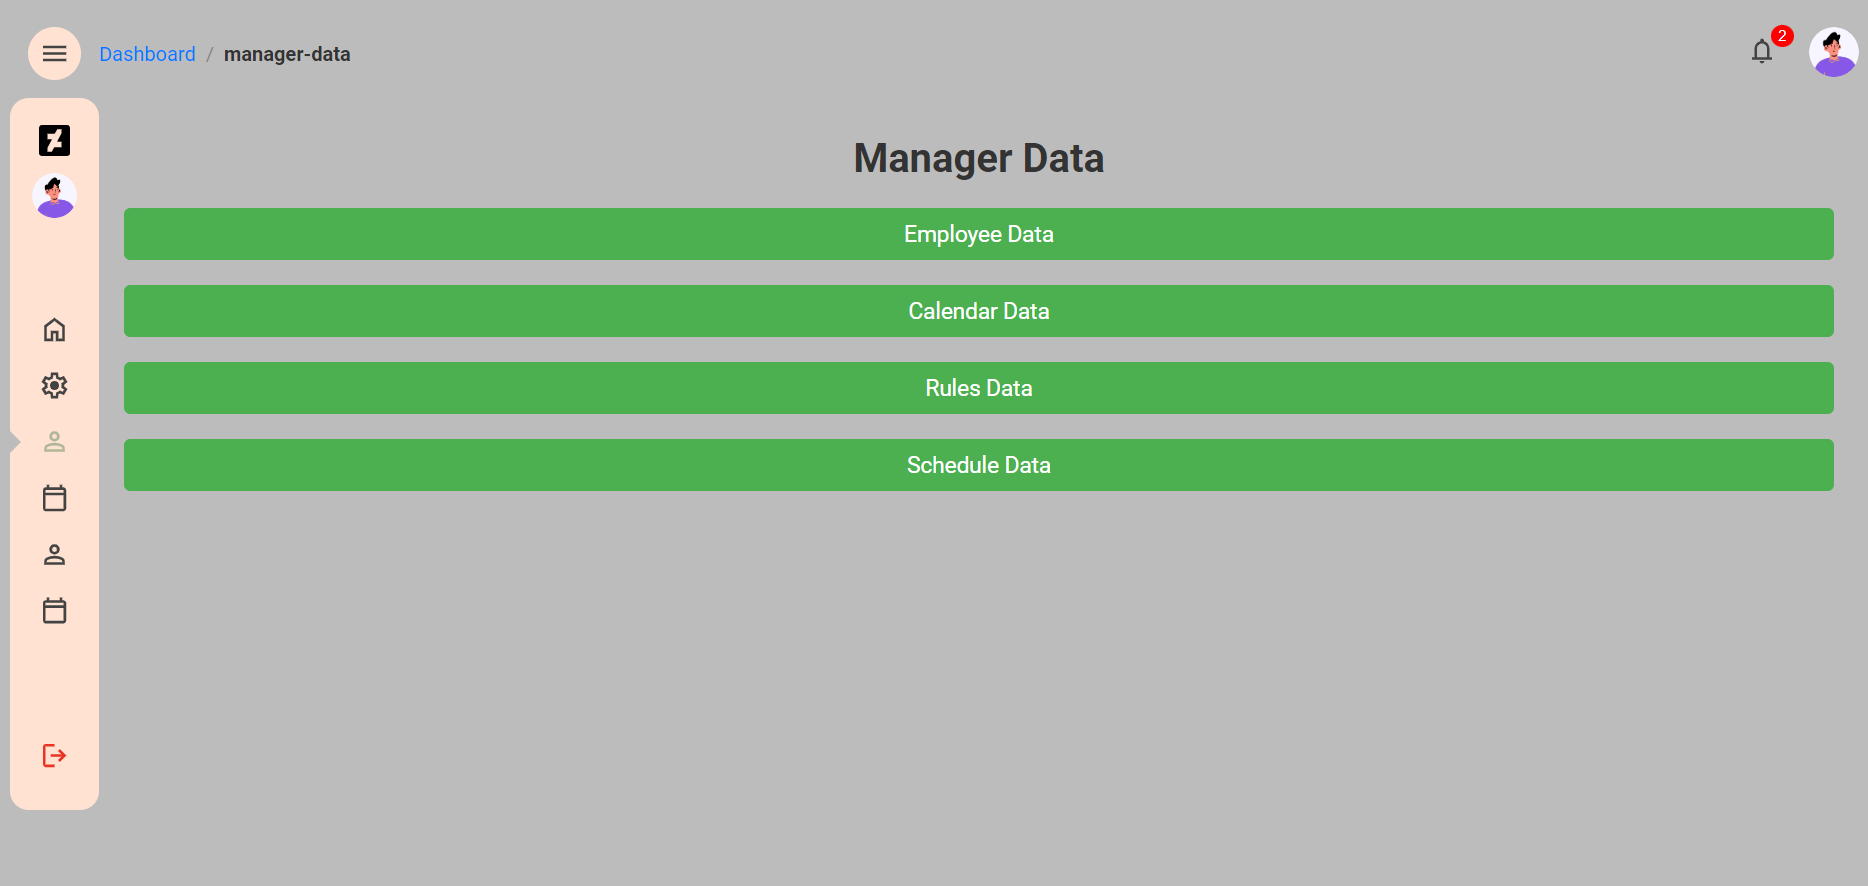
\includegraphics[width=0.8\columnwidth]{ManagerPages/ManagerData.png}
    \caption{Manager Data Page}
    \label{fig:manager-data-page}
    \end{figure}

    For employee data, as illustrated in Figure \ref{fig:manager-employee-data-personal}, managers can export personal data, attendance records, and shift preferences.
    \begin{figure}[H]
    \centering
    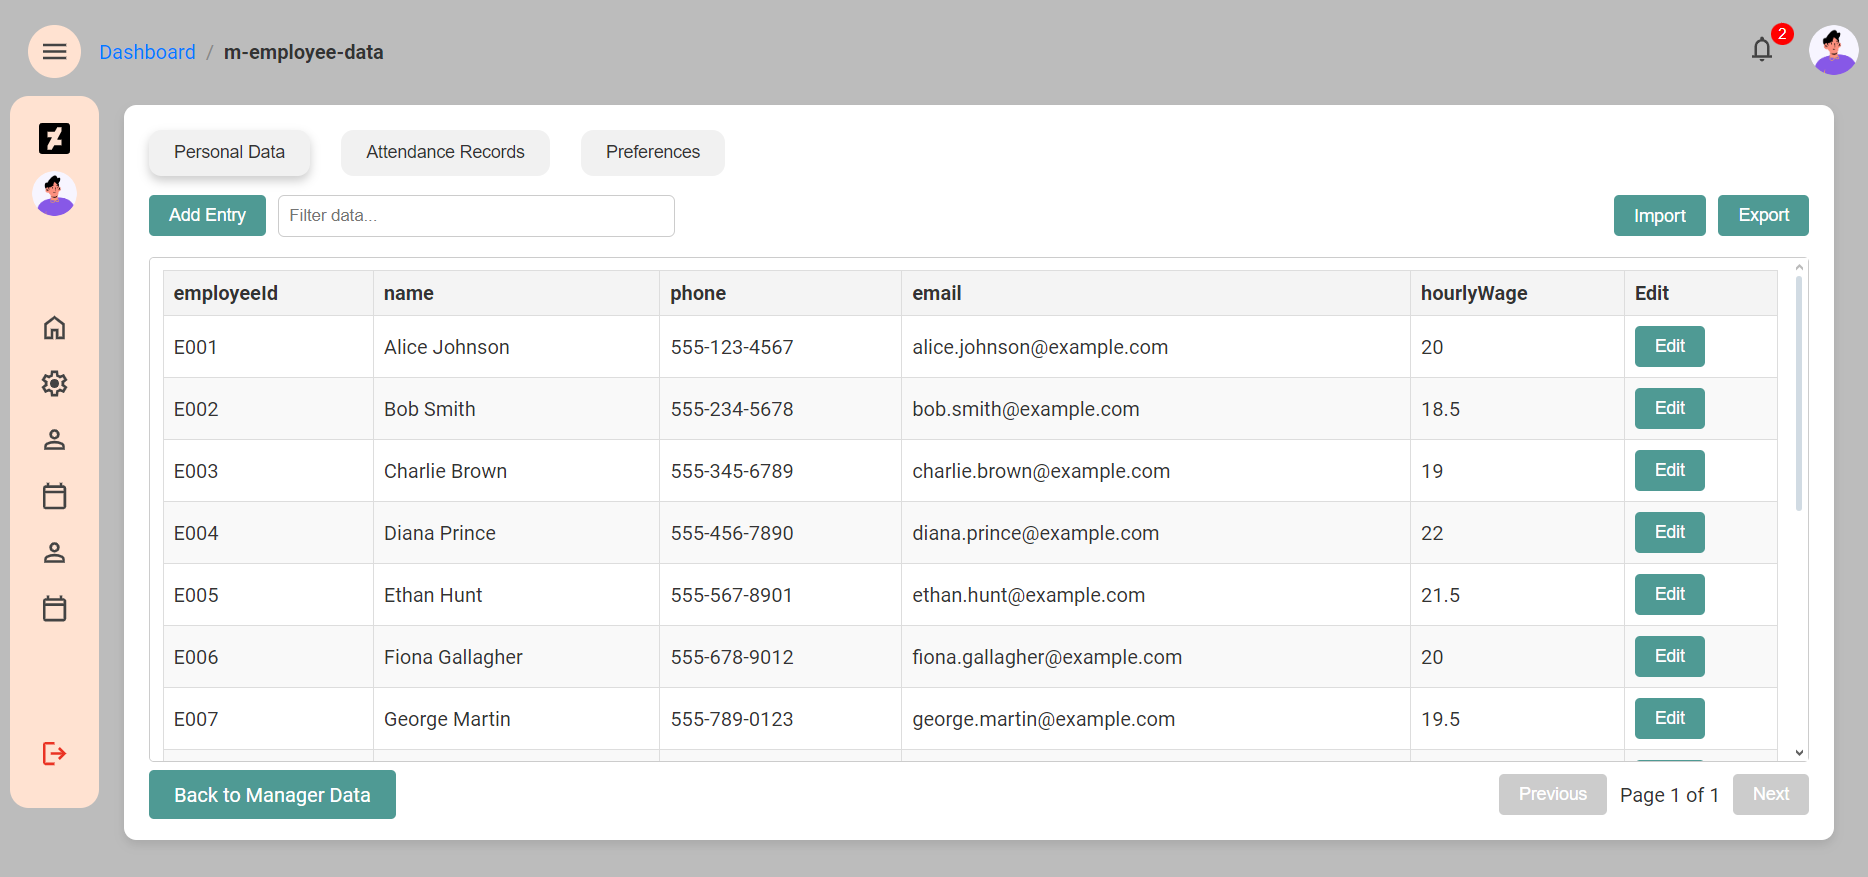
\includegraphics[width=0.8\columnwidth]{ManagerPages/ManagerEmployeeData.png}
    \caption{Manager Data on Employee Personal Data}
    \label{fig:manager-employee-data-personal}
    \end{figure}

    \begin{figure}[H]
    \centering
    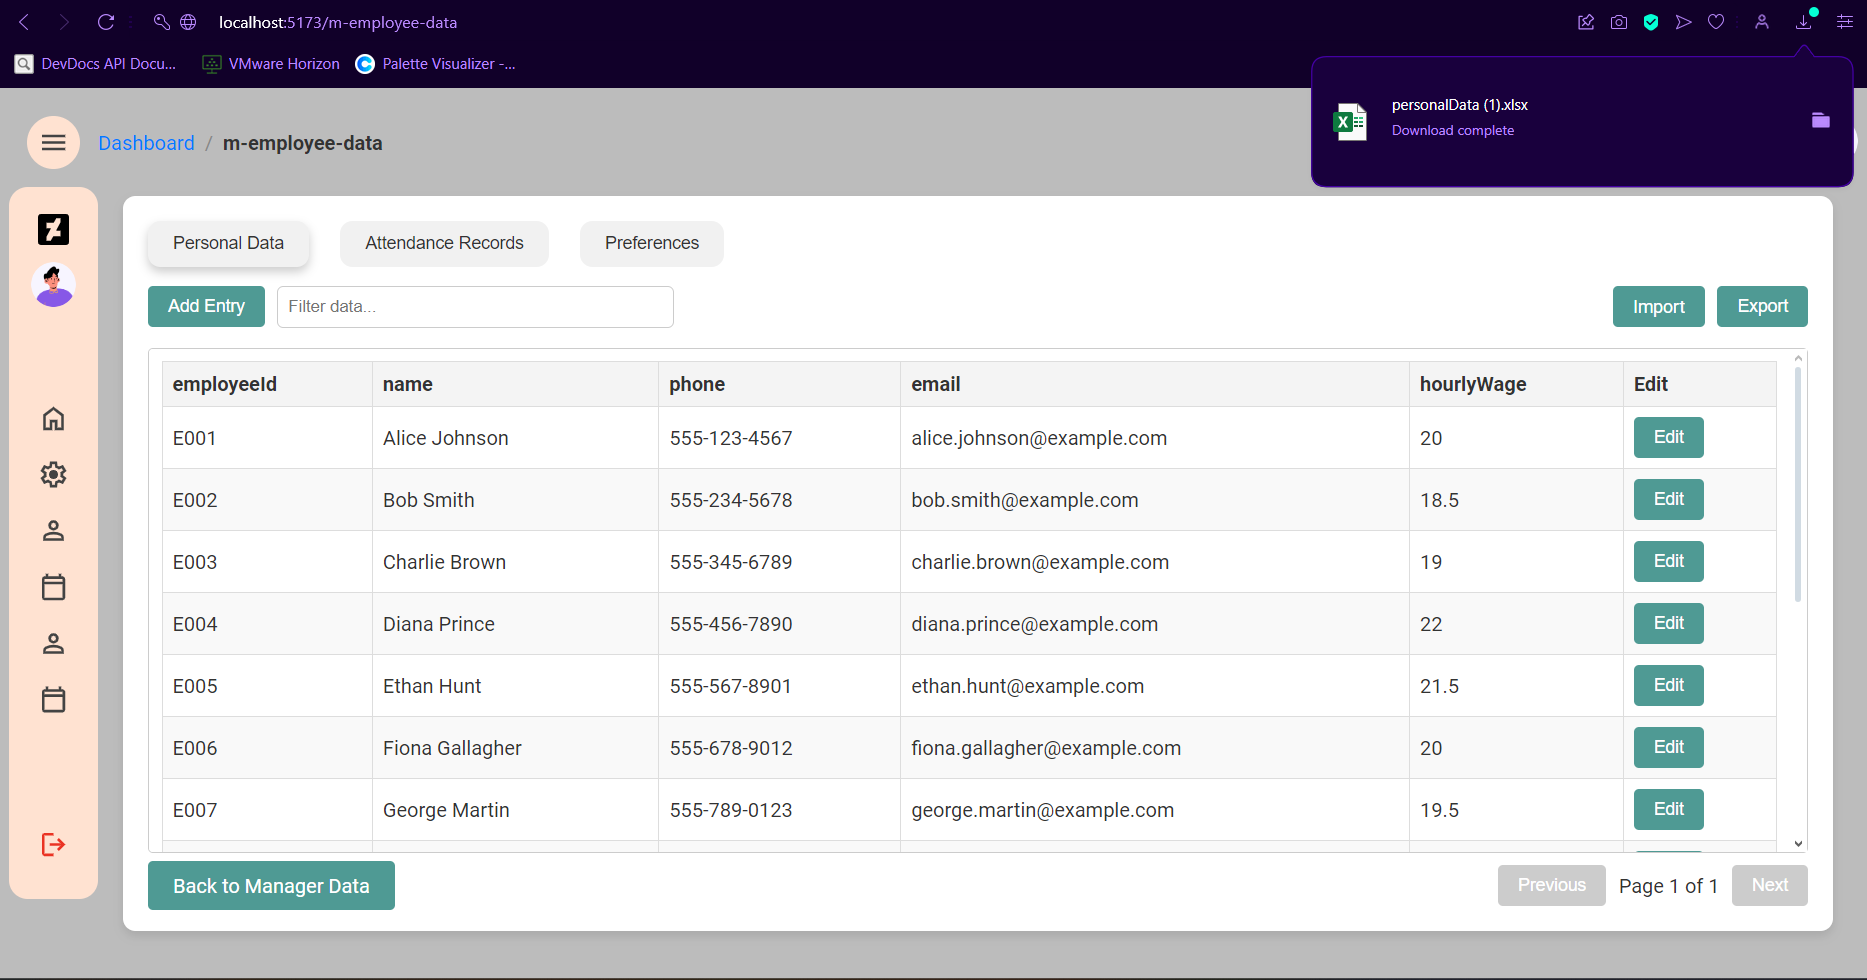
\includegraphics[width=0.8\columnwidth]{ManagerPages/ManagerEmployeeData5.png}
    \caption{Manager Export Employee Personal Data}
    \label{fig:manager-employee-data-personal-export}
    \end{figure}

    \begin{figure}[H]
    \centering
    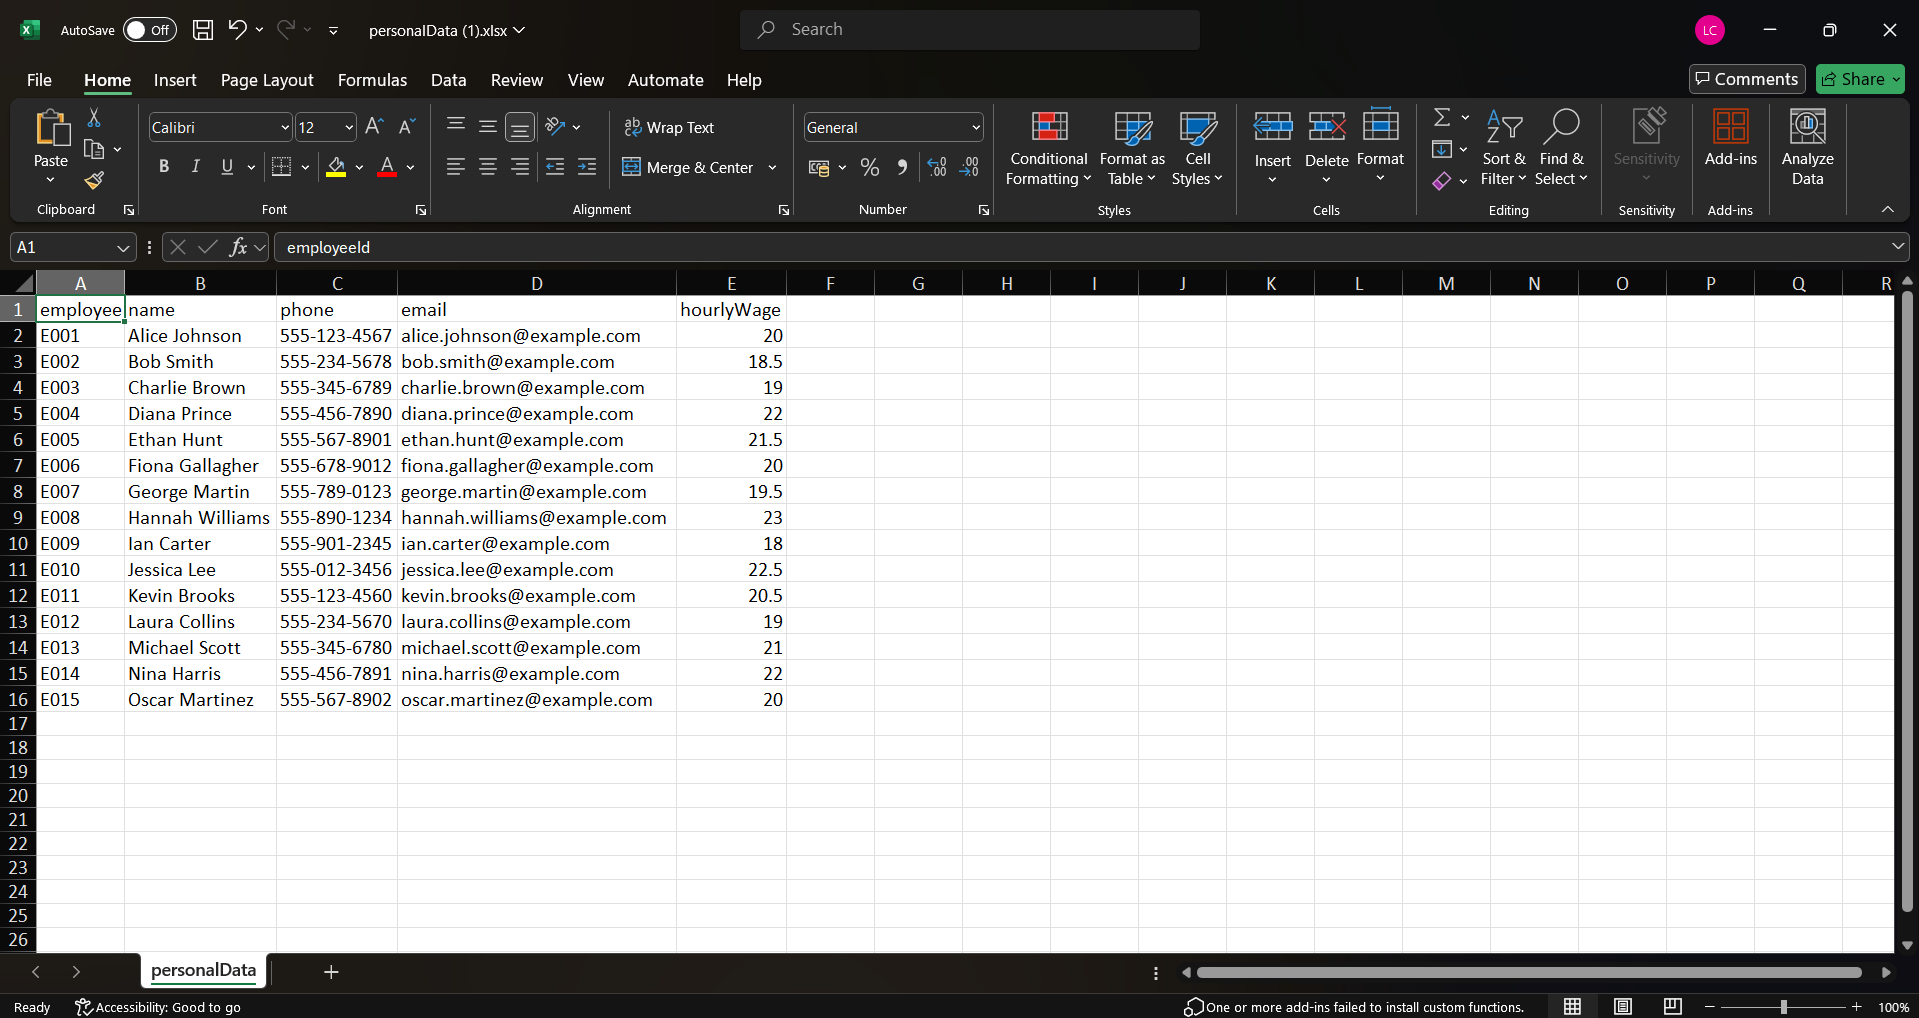
\includegraphics[width=0.8\columnwidth]{ManagerPages/ManagerEmployeeData6.png}
    \caption{Employee Personal Data Excel}
    \label{fig:manager-excel-personal-data}
    \end{figure}

    For the Attendance Records and Preferences, they follow the same procedure to export their data.

    \begin{figure}[H]
    \centering
    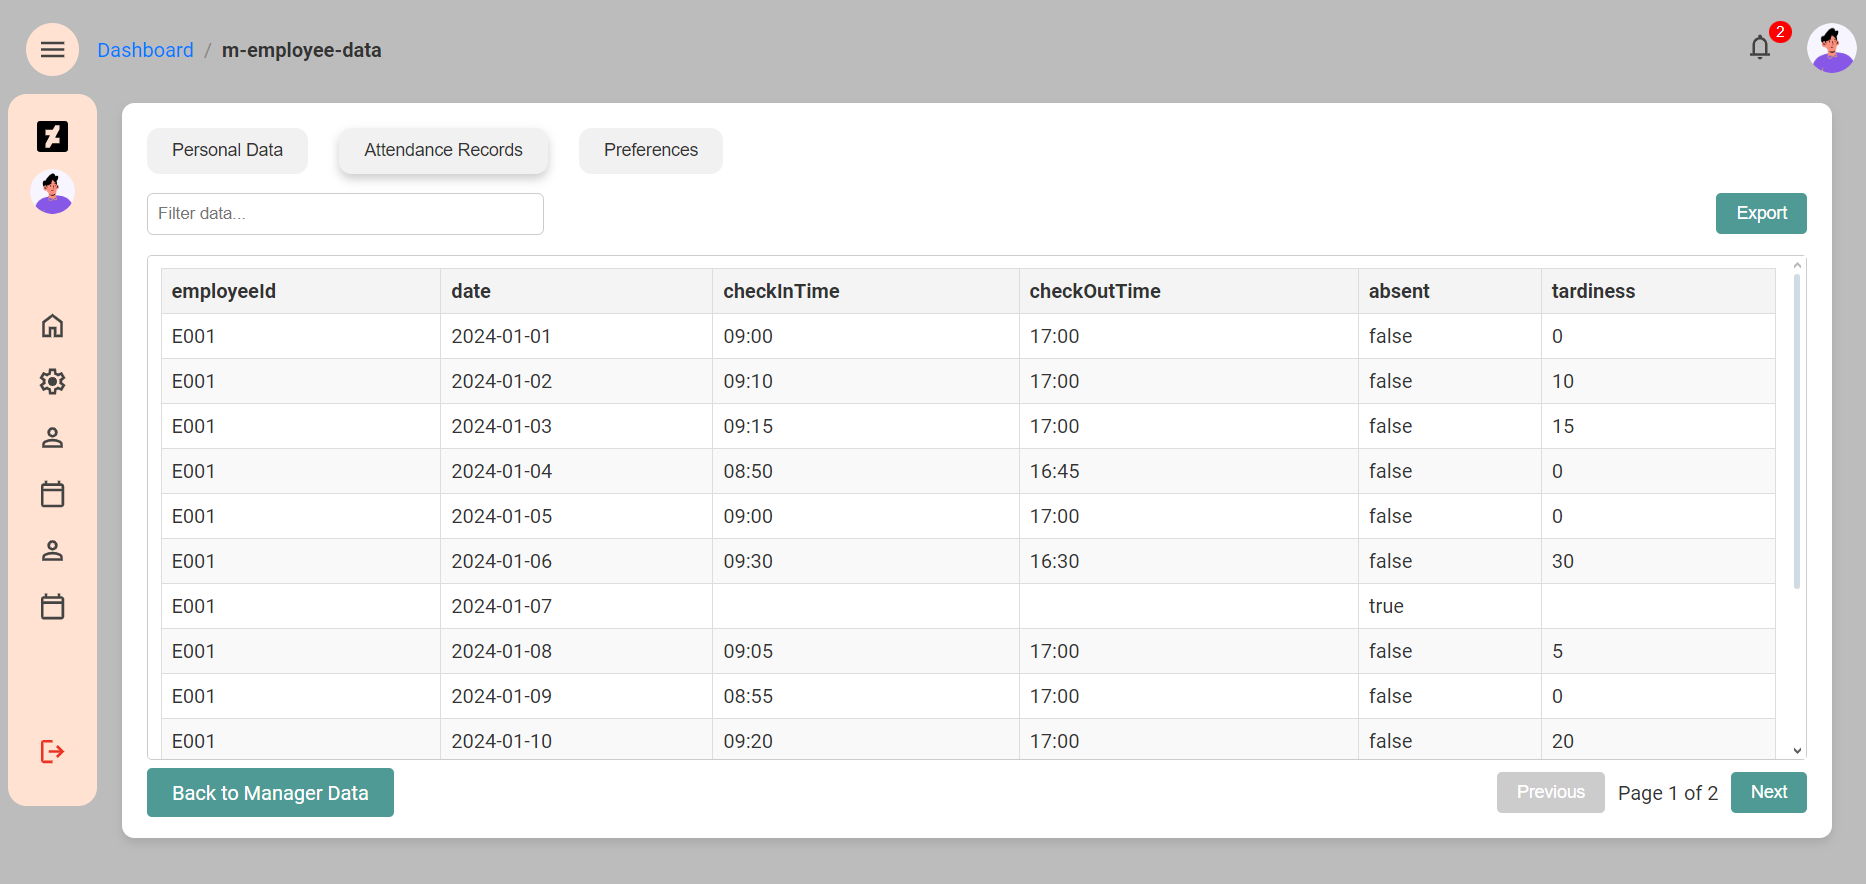
\includegraphics[width=0.8\columnwidth]{ManagerPages/ManagerEmployeeData7.png}
    \caption{Manager Data on Employee Attendance Records}
    \label{fig:manager-employee-data-attendance}
    \end{figure}

    \begin{figure}[H]
    \centering
    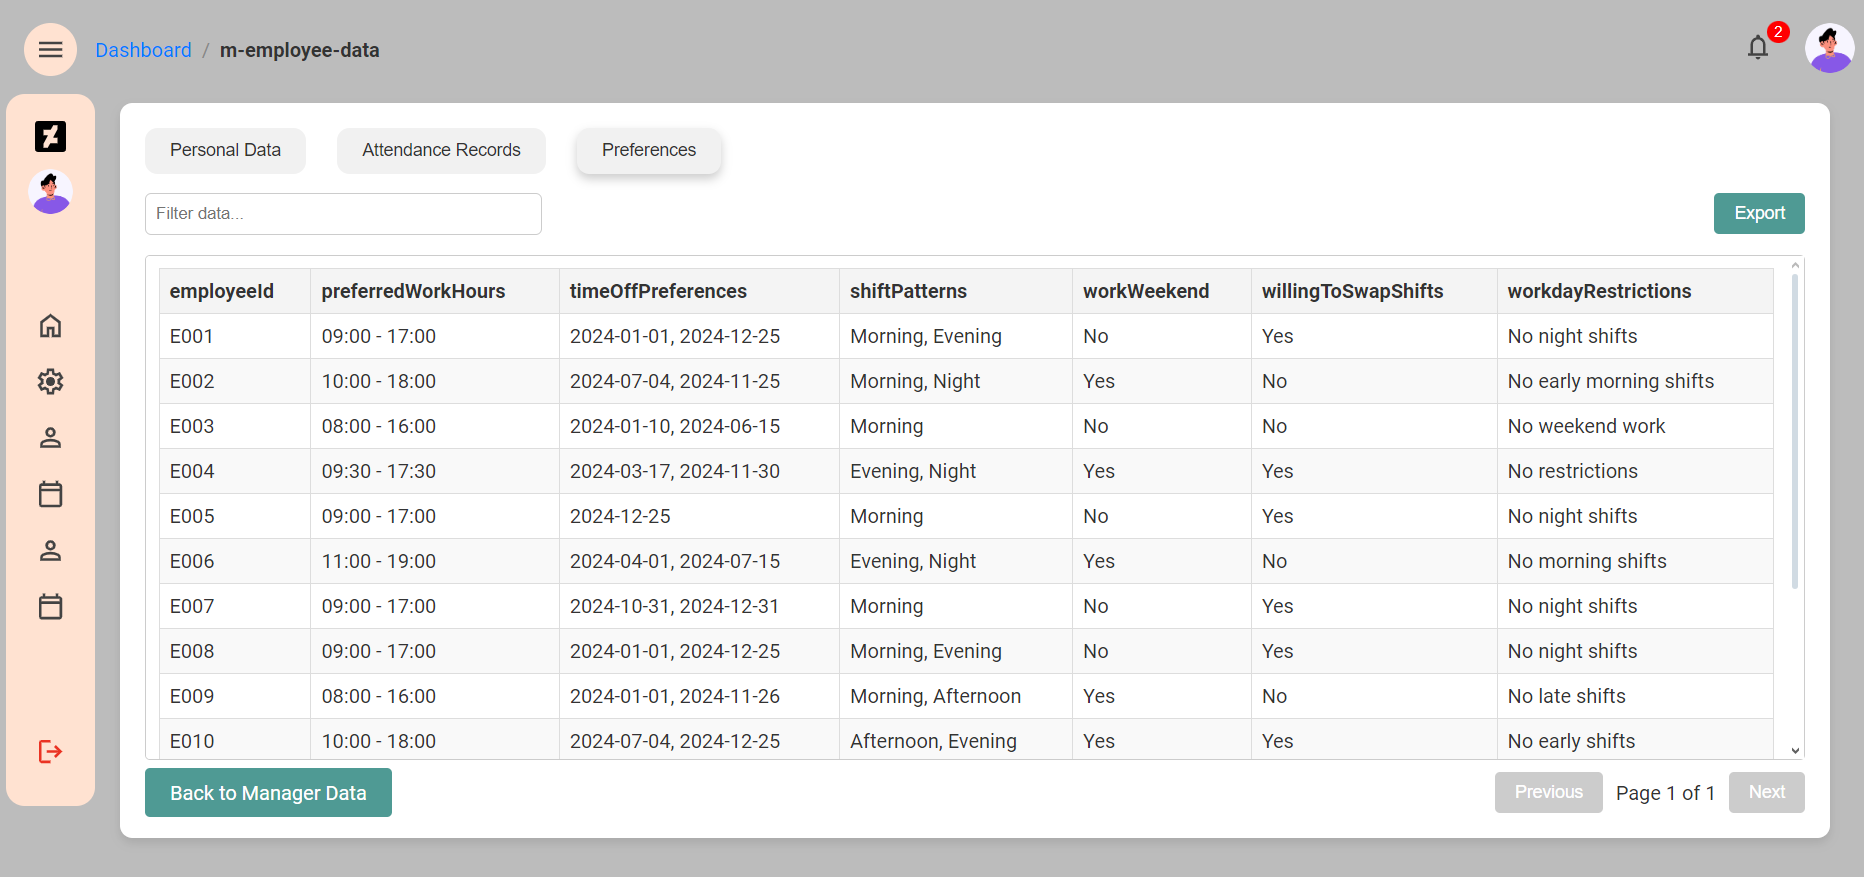
\includegraphics[width=0.8\columnwidth]{ManagerPages/ManagerEmployeeData8.png}
    \caption{Manager Data on Employee Preferences}
    \label{fig:manager-employee-data-preferences}
    \end{figure}

    For calendar data in figure \ref{fig:manager-calendar-data-form}, manager are able to edit holiday details.
    \begin{figure}[H]
    \centering
    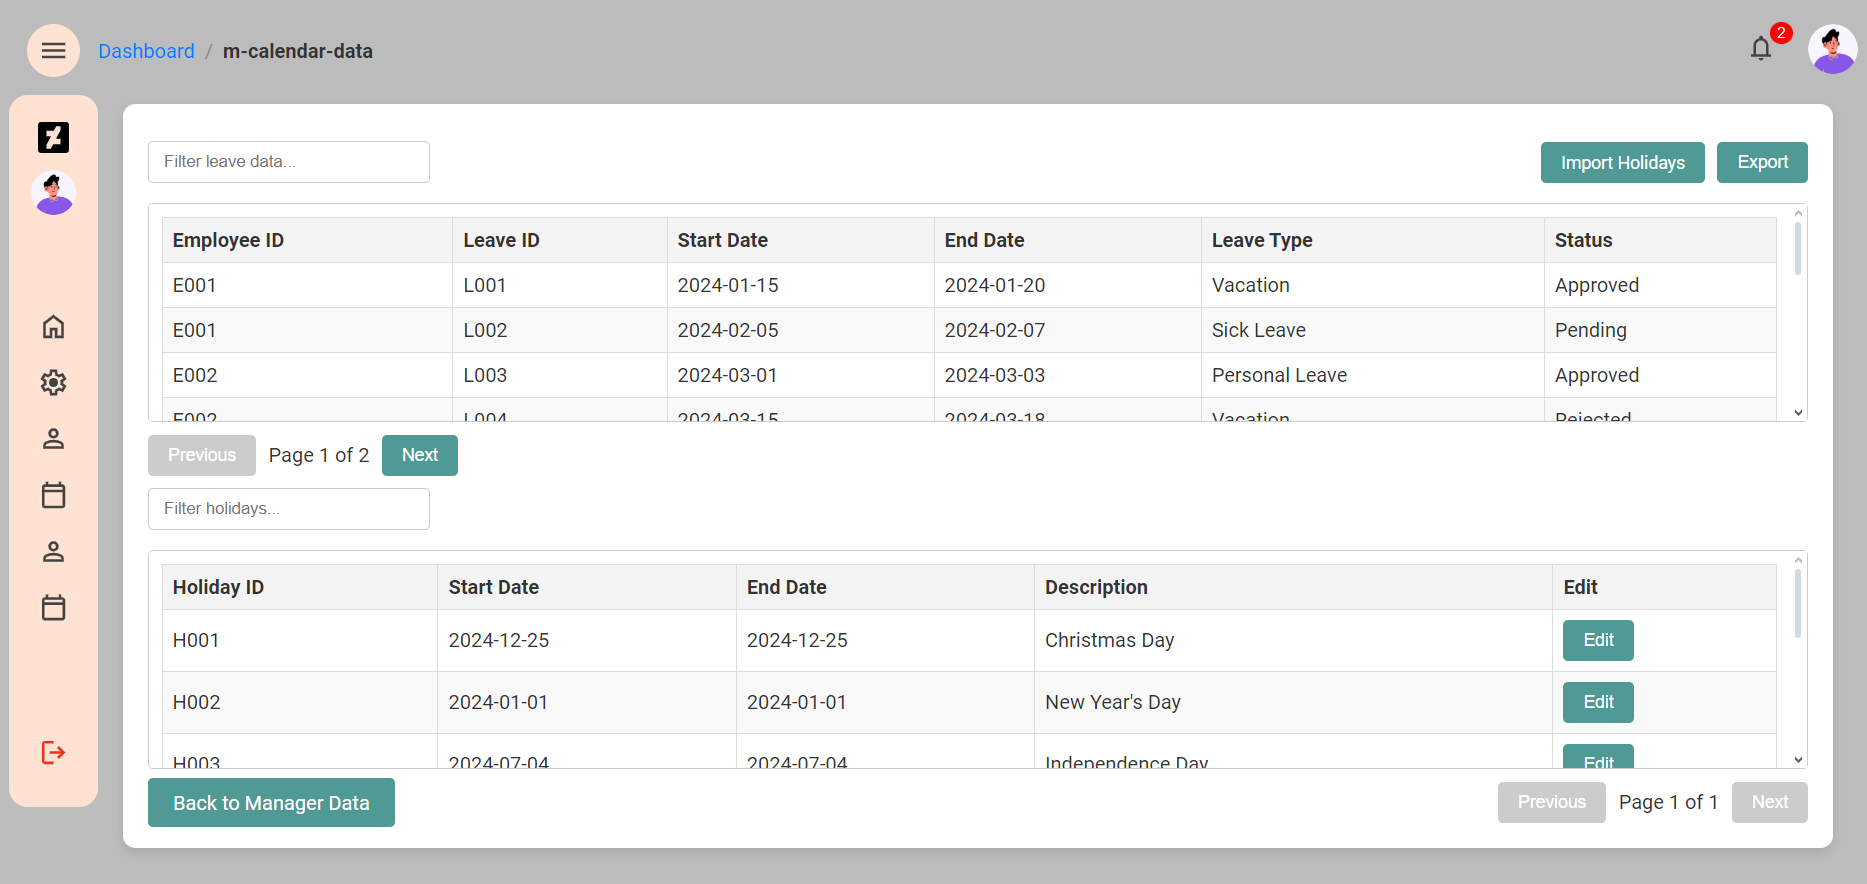
\includegraphics[width=0.8\columnwidth]{ManagerPages/ManagerCalendarData.png}
    \caption{Manager Data on Calendar Data}
    \label{fig:manager-calendar-data}
    \end{figure}

    \begin{figure}[H]
    \centering
    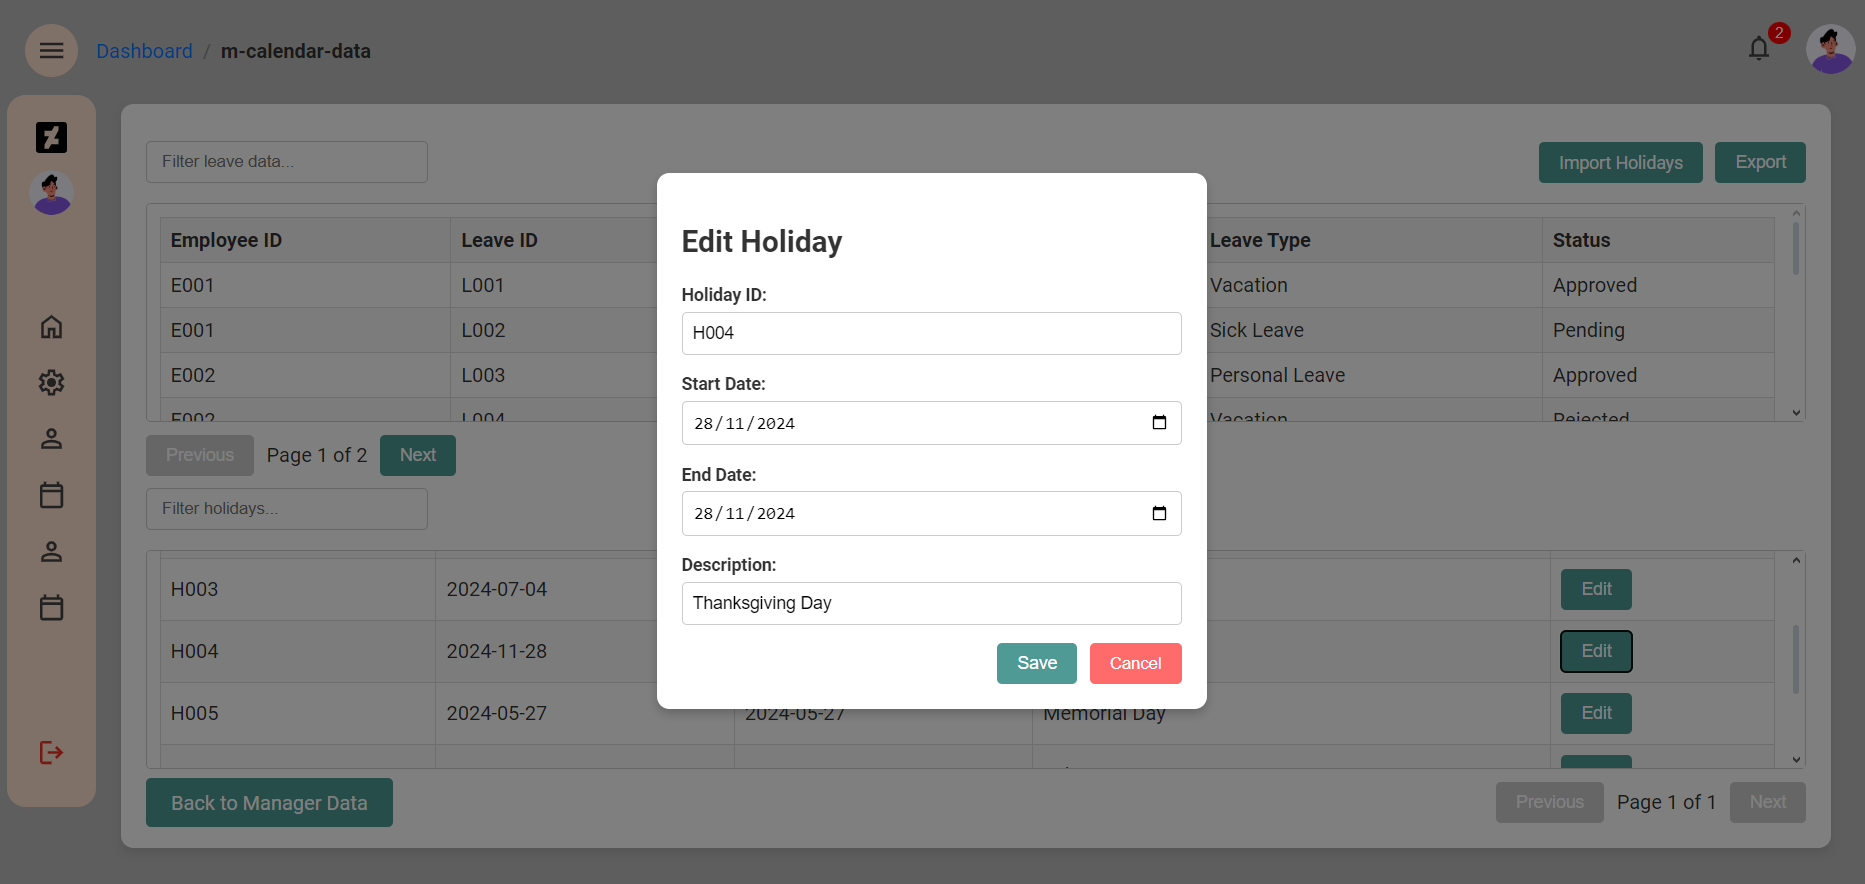
\includegraphics[width=0.8\columnwidth]{ManagerPages/ManagerCalendarData2.png}
    \caption{Manager Edit Holiday Data Form}
    \label{fig:manager-calendar-data-form}
    \end{figure}

    As illustrated in Figure \ref{fig:manager-rules-data} , manager are able to edit and add both rules and demands.Additionally, managers can use filter to efficiently locate specific rules and demands.
    \begin{figure}[H]
    \centering
    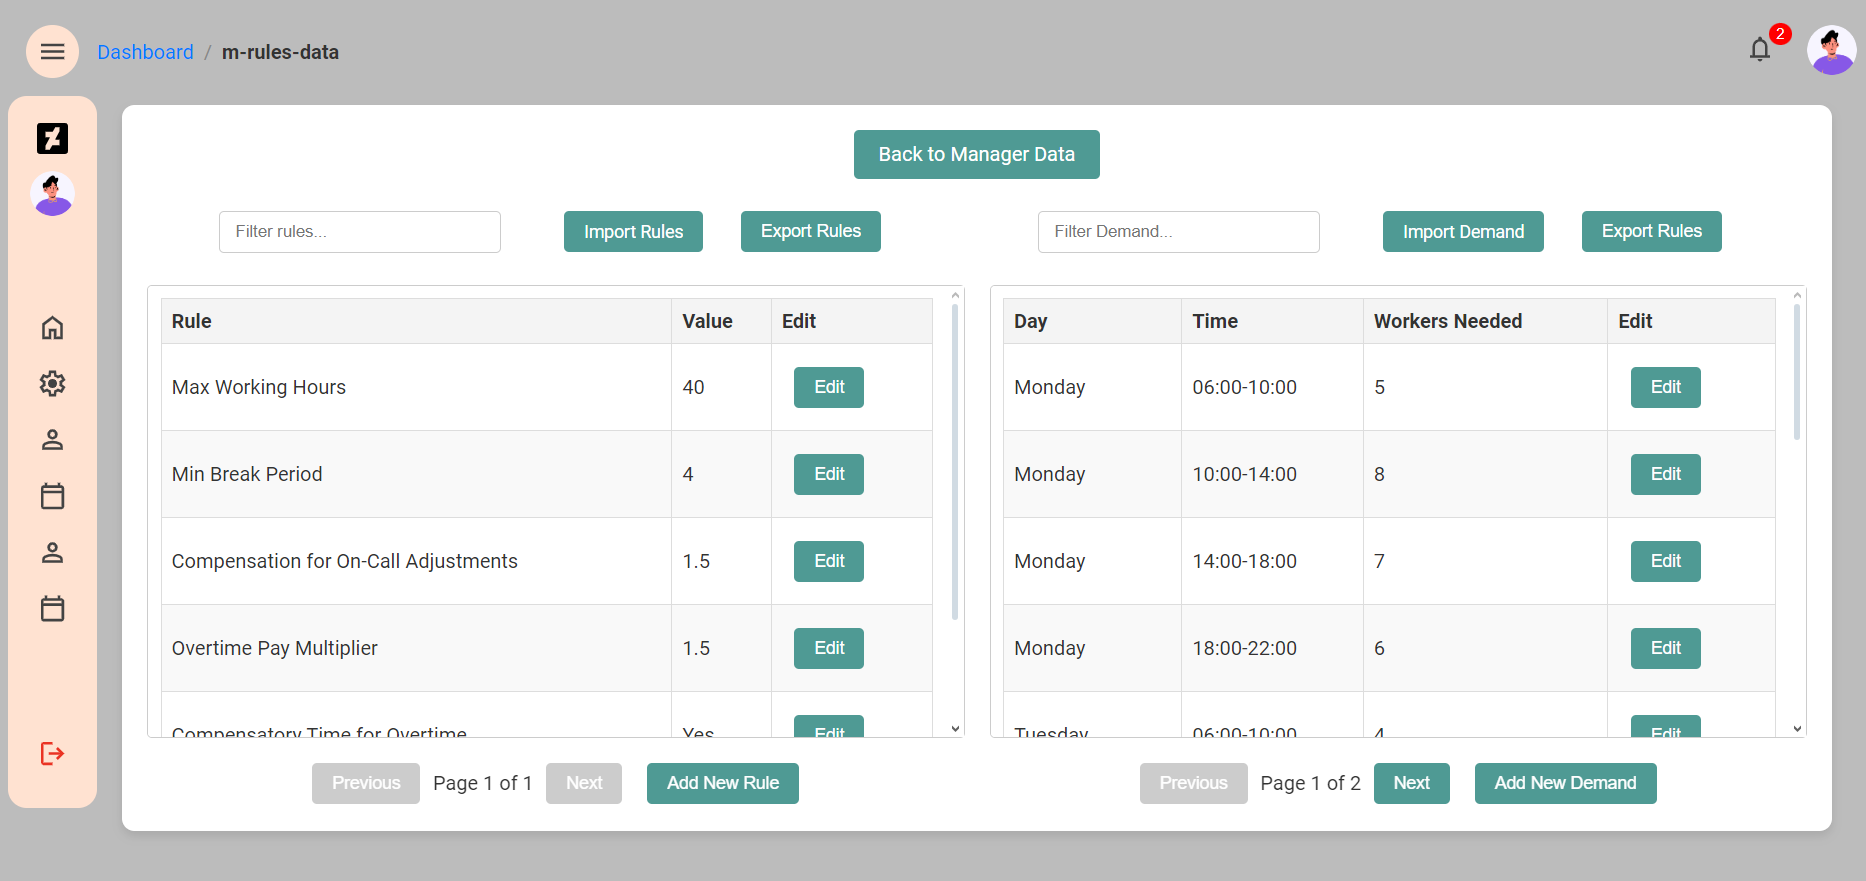
\includegraphics[width=0.8\columnwidth]{ManagerPages/ManagerRulesData.png}
    \caption{Manager Data on Rules}
    \label{fig:manager-rules-data}
    \end{figure}
    
    \begin{figure}[H]
    \centering
    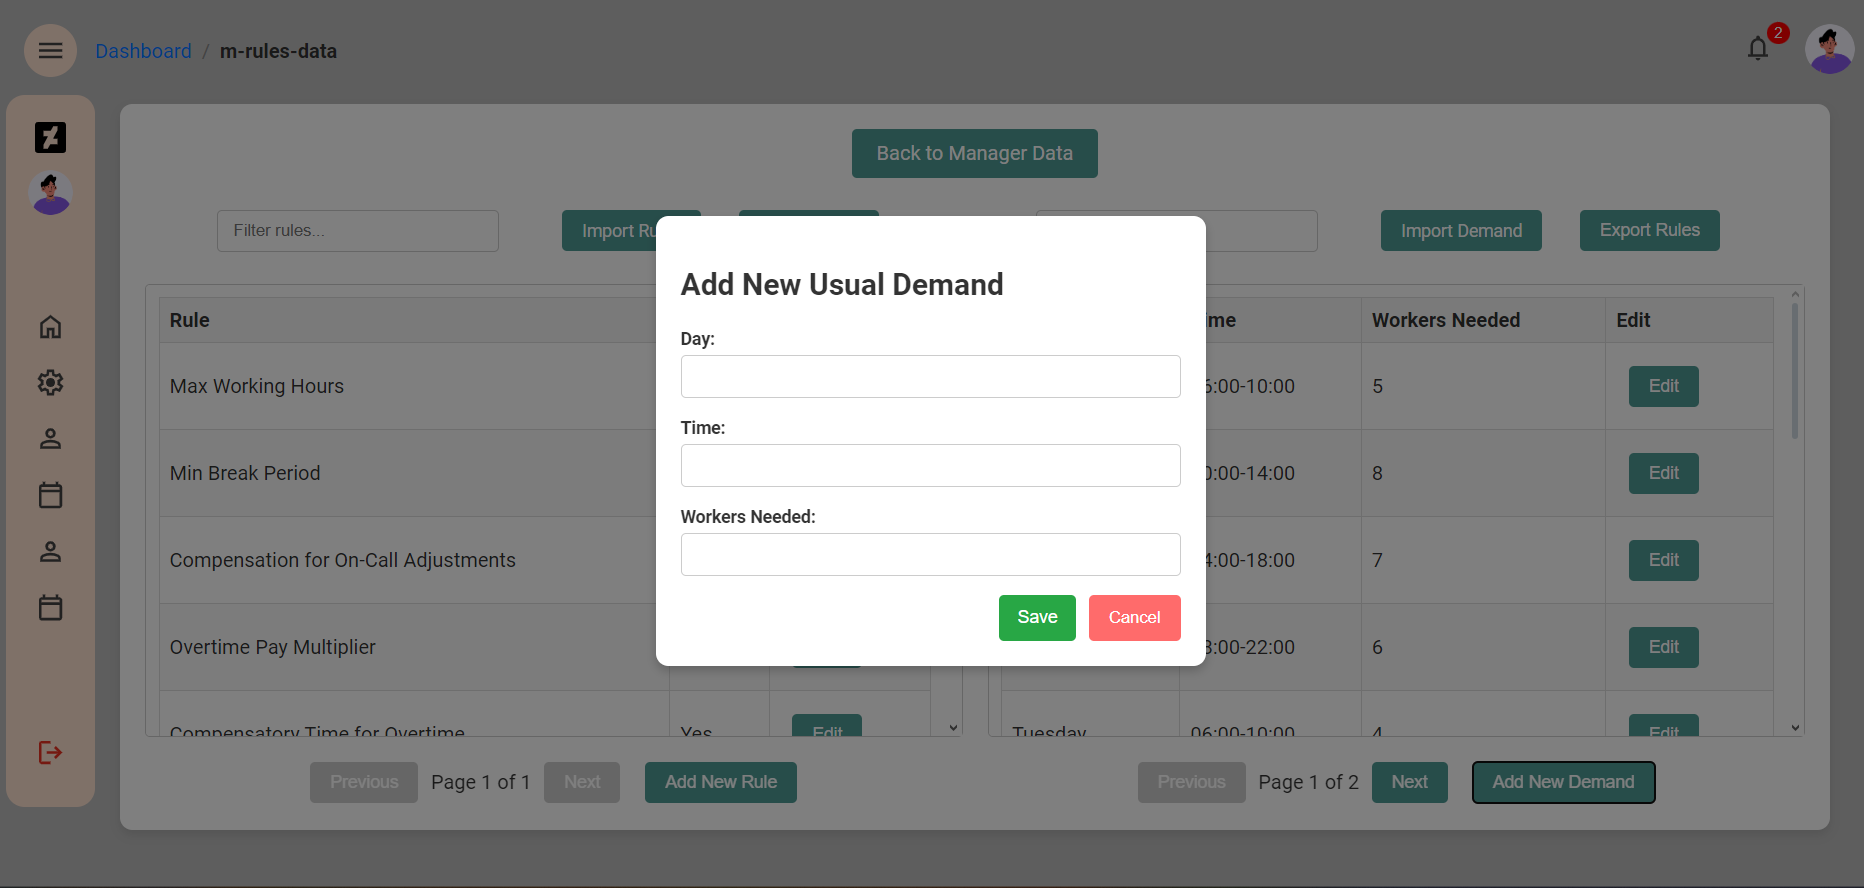
\includegraphics[width=0.8\columnwidth]{ManagerPages/ManagerRulesData2.png}
    \caption{Manager Add New Demand}
    \label{fig:manager-new-demand}
    \end{figure}

    \begin{figure}[H]
    \centering
    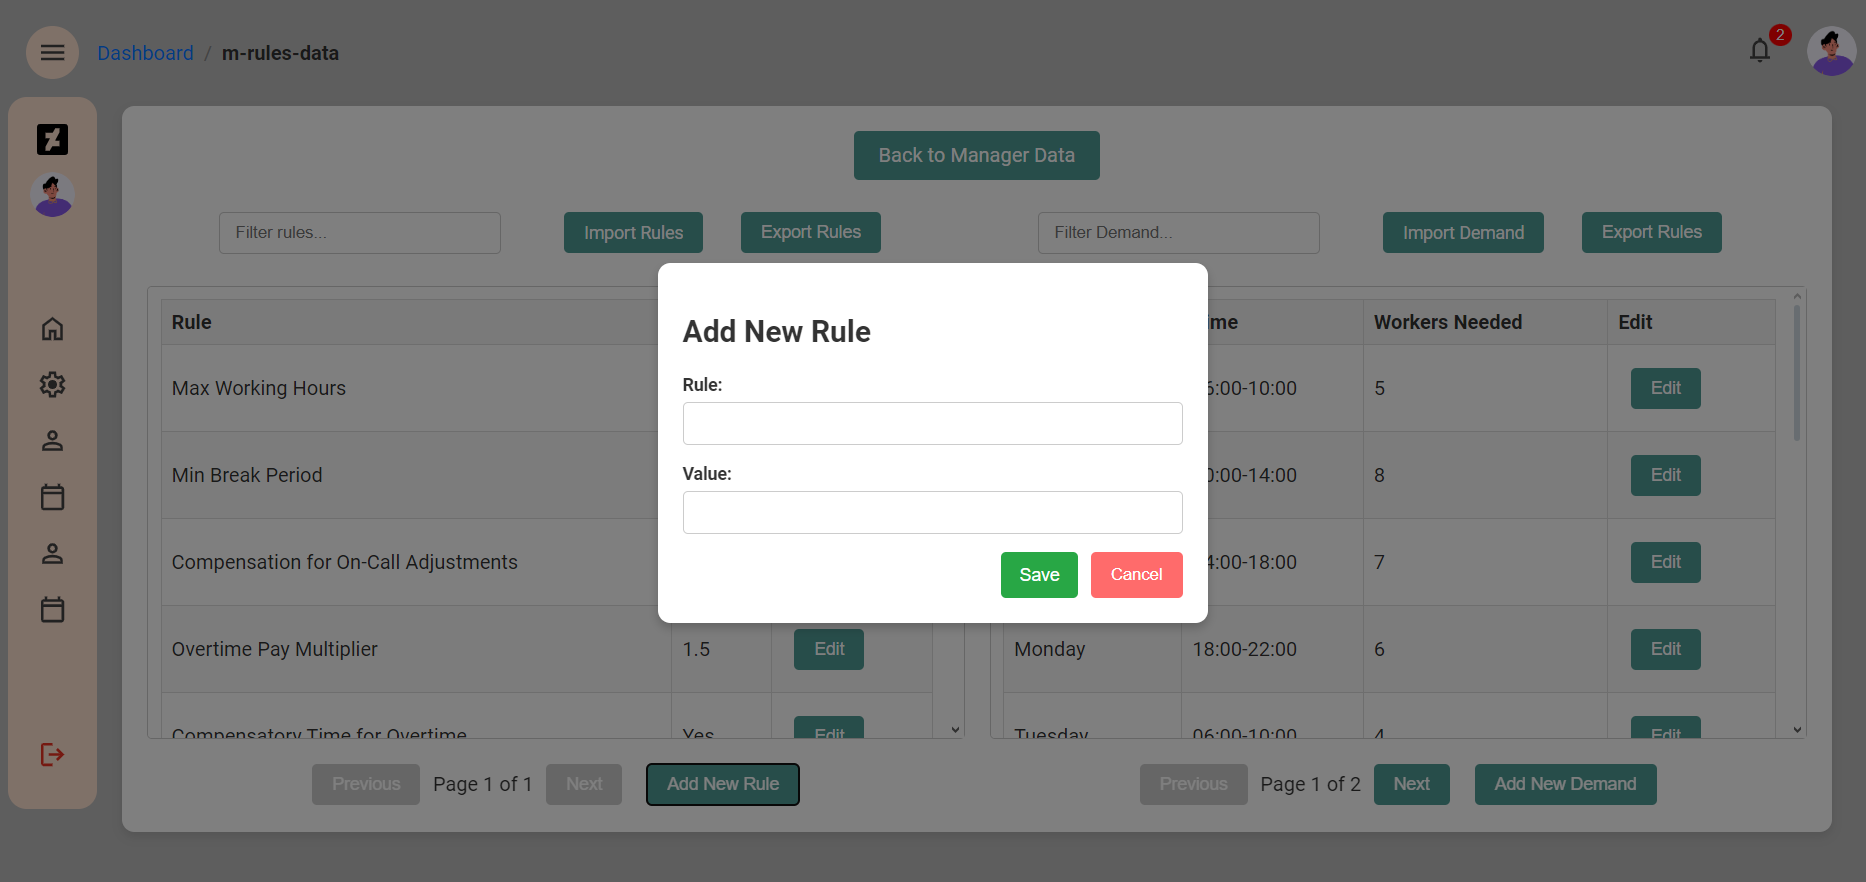
\includegraphics[width=0.8\columnwidth]{ManagerPages/ManagerRulesData3.png}
    \caption{Manager Add New Rule}
    \label{fig:manager-new-rules}
    \end{figure}

   As shown in Figure \ref{fig:manager-employee-schedules-c}, managers can export or import employee schedules as well as the regular weekly schedule, shown in figure \ref{fig:manager-usual-schedules}.
    \begin{figure}[H]
    \centering
    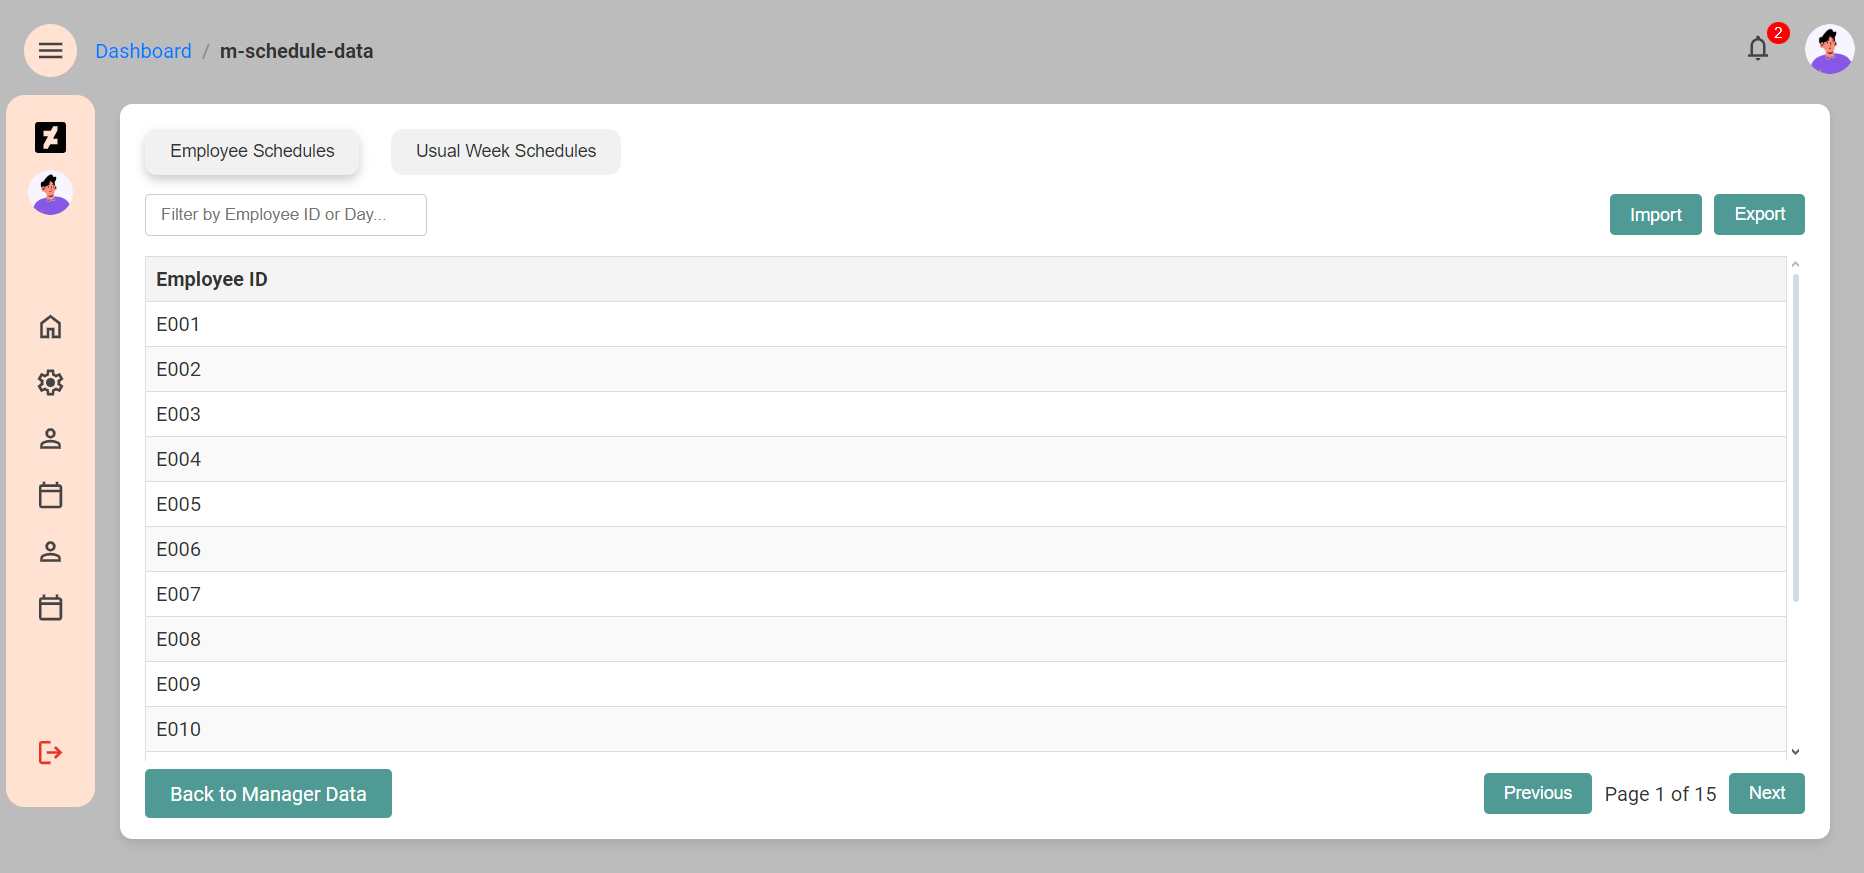
\includegraphics[width=0.8\columnwidth]{ManagerPages/ManagerScheduleData.png}
    \caption{Manager Data on Employee Schedules Collapsed}
    \label{fig:manager-employee-schedules-c}
    \end{figure}

    \begin{figure}[H]
    \centering
    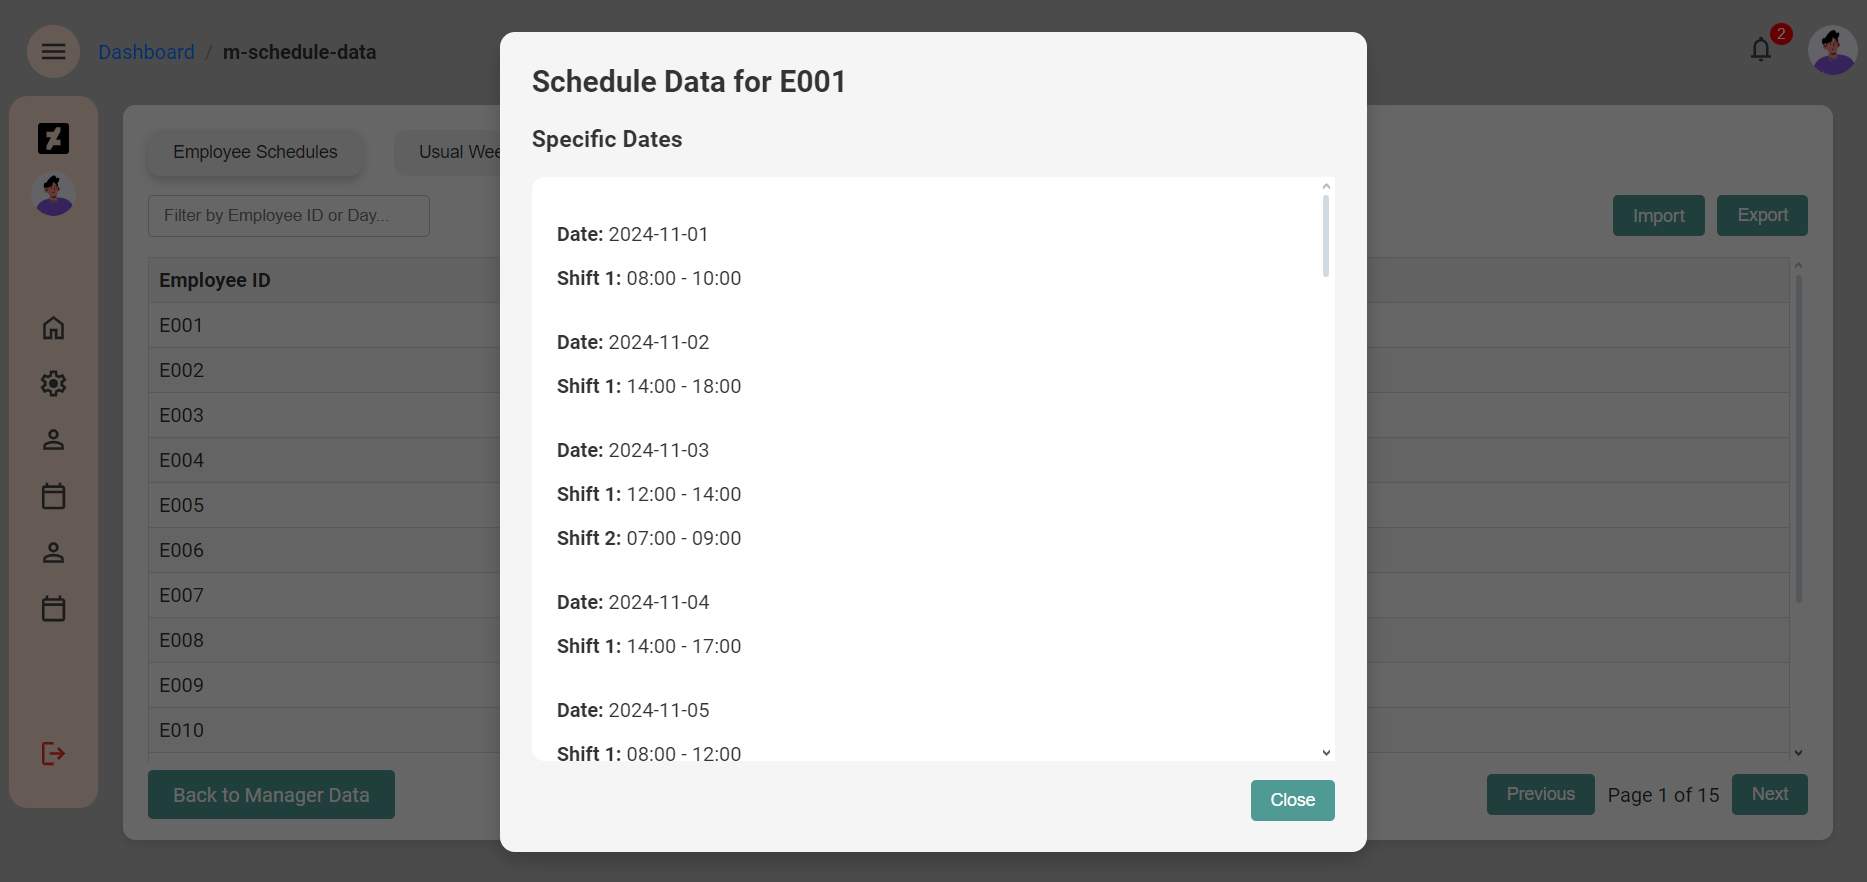
\includegraphics[width=0.8\columnwidth]{ManagerPages/ManagerScheduleData2.png}
    \caption{Manager Data on Employee Schedules Expanded}
    \label{fig:manager-employee-schedules-e}
    \end{figure}

    \begin{figure}[H]
    \centering
    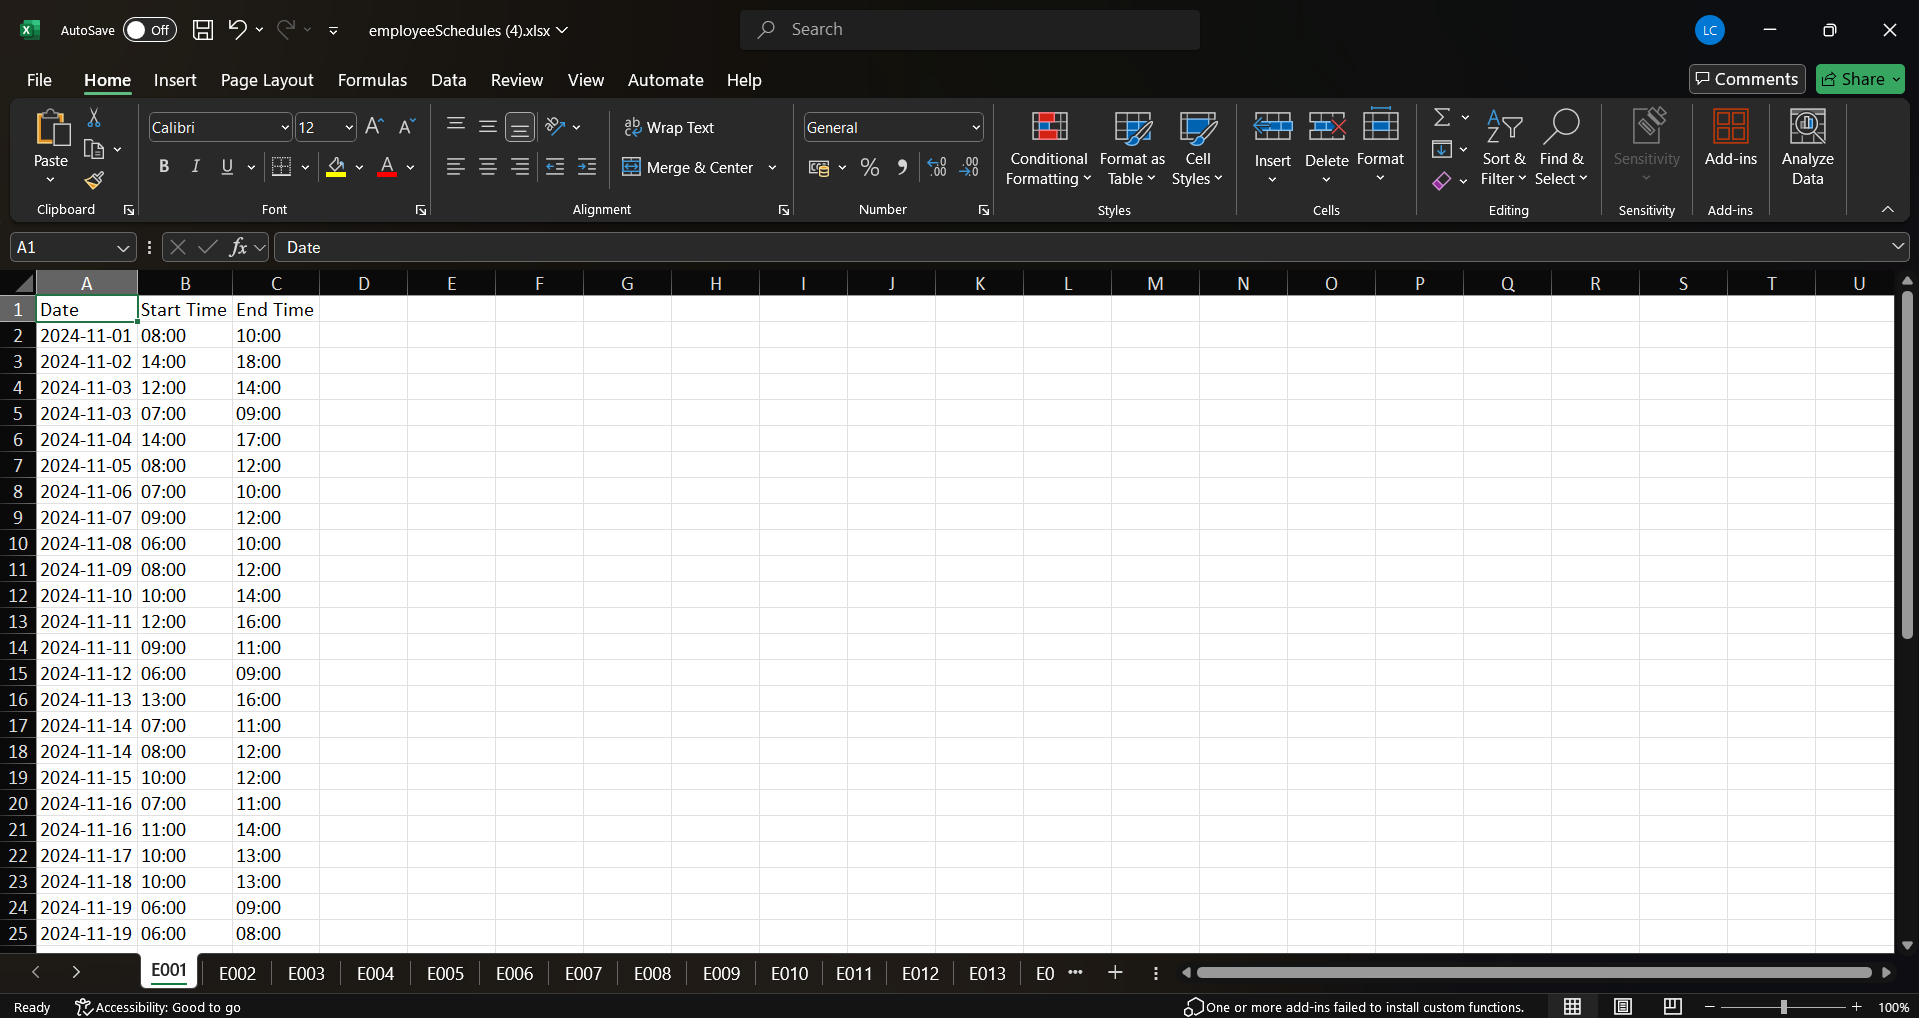
\includegraphics[width=0.8\columnwidth]{ManagerPages/ManagerScheduleData4.png}
    \caption{Employee Schedules Exported Excel}
    \label{fig:manager-employee-schedules-excel}
    \end{figure}

    \begin{figure}[H]
    \centering
    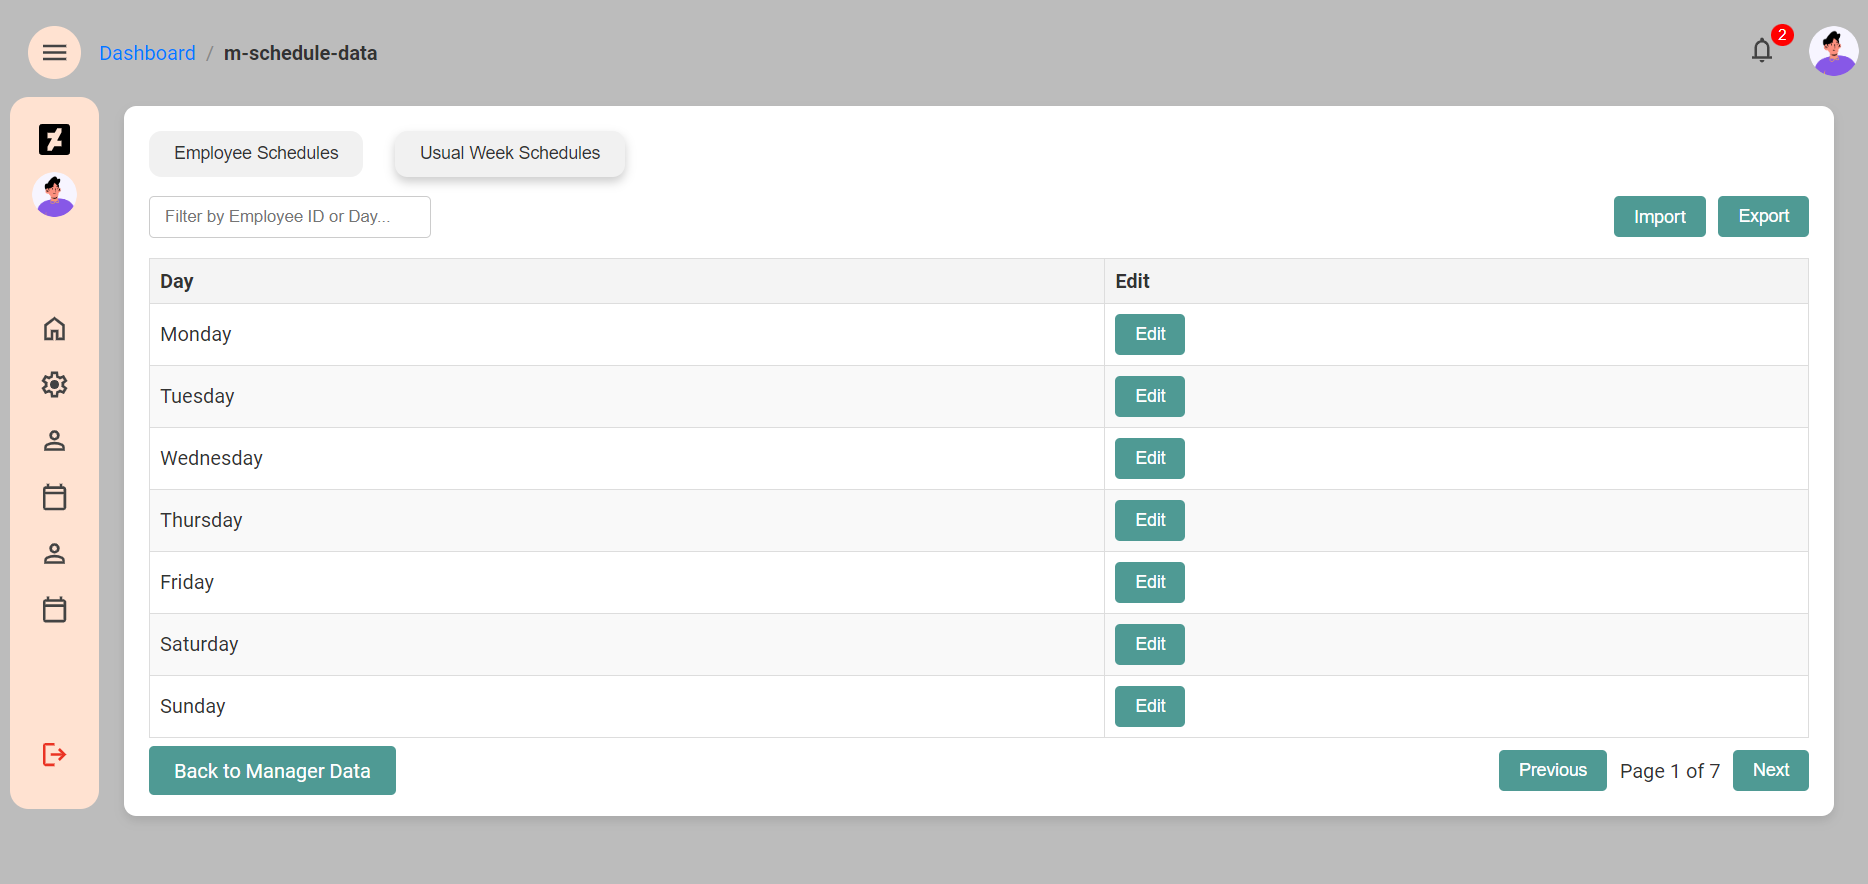
\includegraphics[width=0.8\columnwidth]{ManagerPages/ManagerScheduleData5.png}
    \caption{Manager Data on Usual Schedules}
    \label{fig:manager-usual-schedules}
    \end{figure}

    \begin{figure}[H]
    \centering
    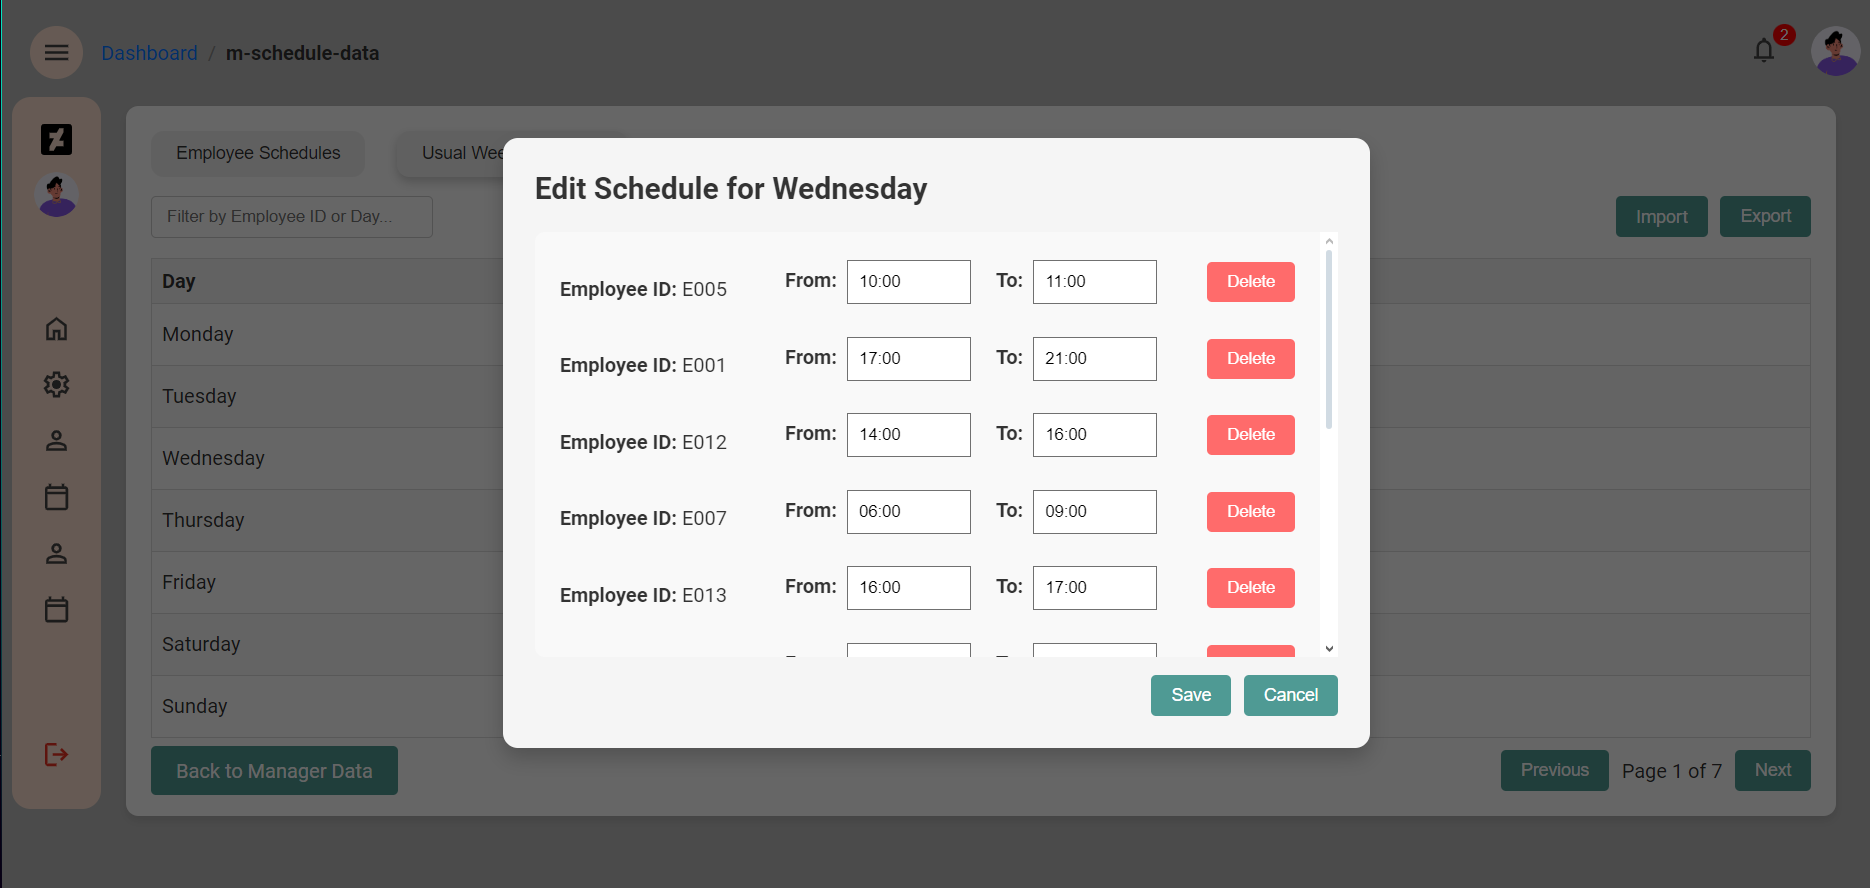
\includegraphics[width=0.8\columnwidth]{ManagerPages/ManagerScheduleData6.png}
    \caption{Manager Edit Usual Schedule}
    \label{fig:manager-usual-schedule-edit}
    \end{figure}

    
    \item \textbf{Profile Viewing:} Enables managers to view personal details, team overview, weekly overview and edit profile.
    \begin{figure}[H]
    \centering
    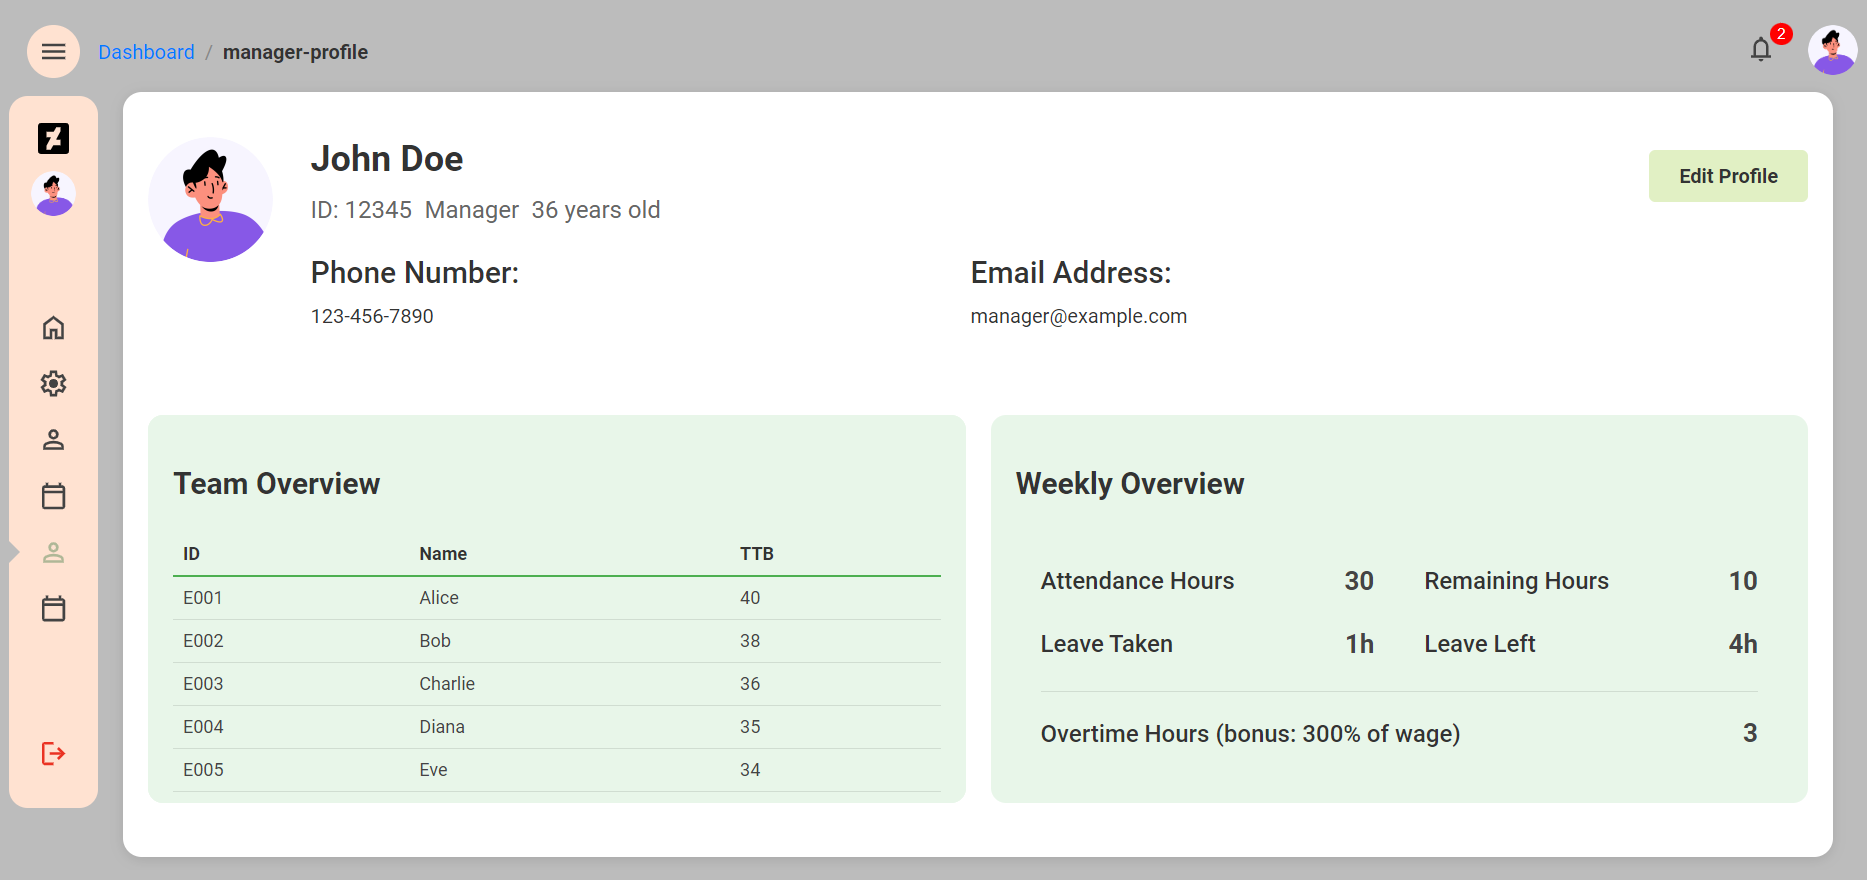
\includegraphics[width=0.8\columnwidth]{ManagerPages/ManagerProfile.png}
    \caption{Manager Profile Page}
    \label{fig:manager-profile}
    \end{figure}

    \begin{figure}[H]
    \centering
    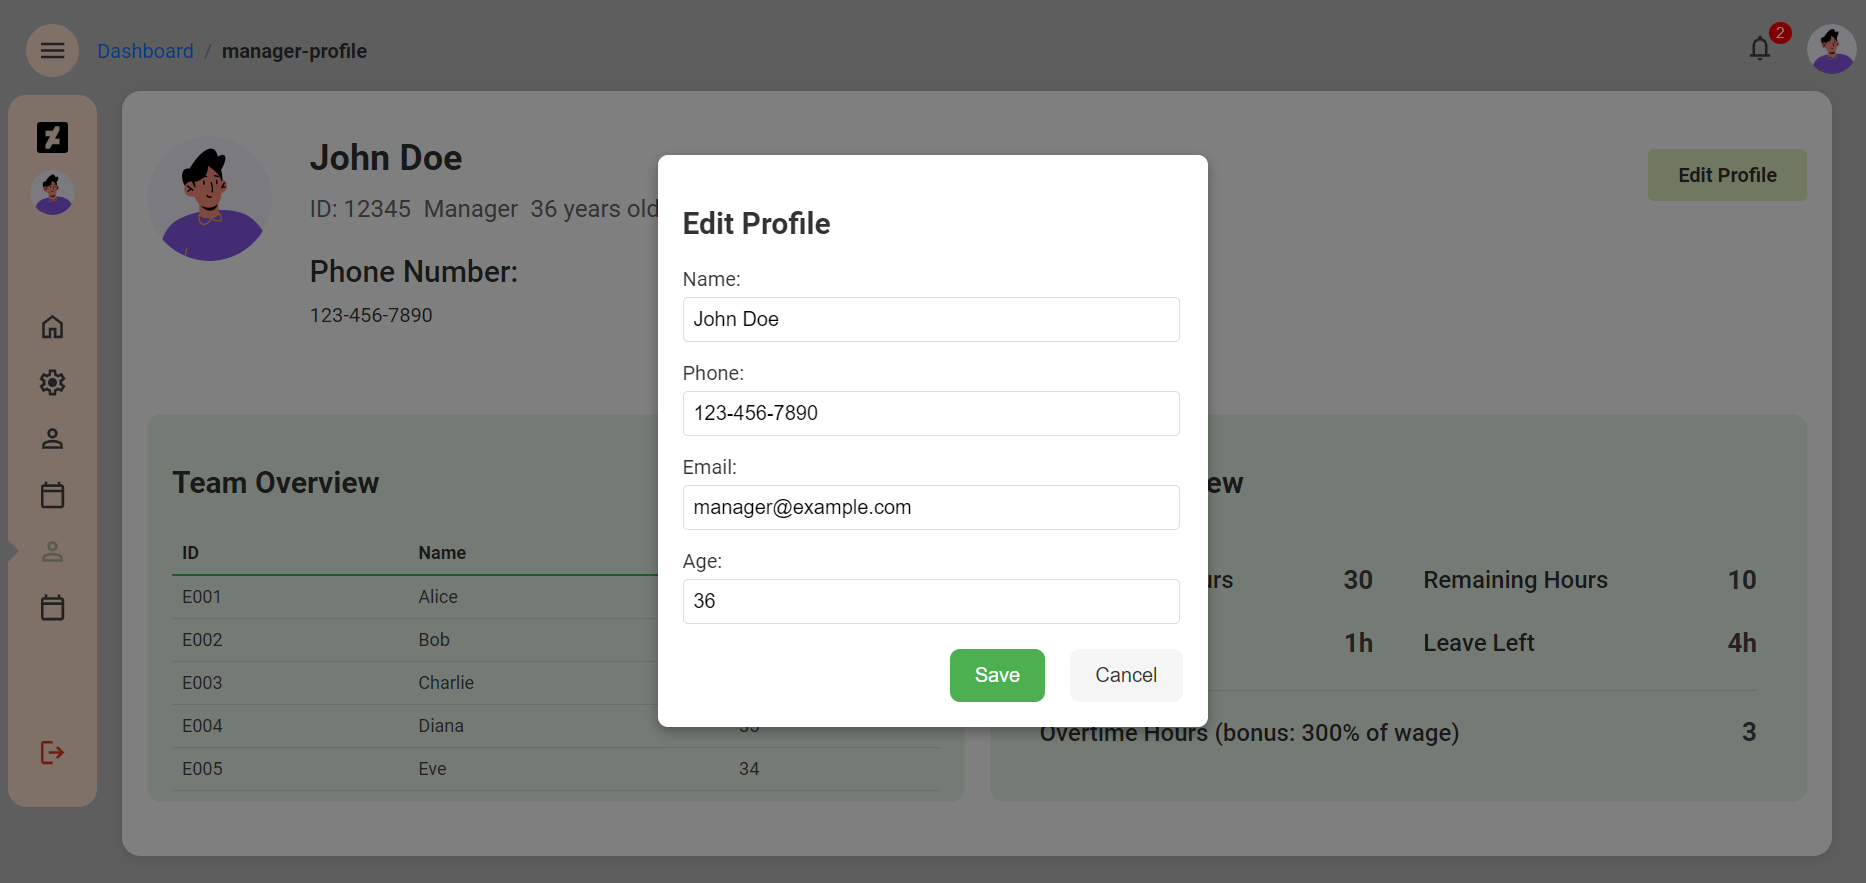
\includegraphics[width=0.8\columnwidth]{ManagerPages/ManagerProfile2.png}
    \caption{Manager Edit Profile}
    \label{fig:manager-profile-edit}
    \end{figure}
    
\end{itemize}

\subsection{Stakeholder Feedback}
\begin{itemize}
    \item Positive feedback on the ability for employees to choose between daily, weekly, or monthly views of their schedules.
    \item Requests for notification systems when manager approve or deny leave requests, assign new shifts or approve shift swap.
    \item Appreciate for the feature that allows data export and import
\end{itemize}

\subsection{Challenges and Fixes}
    \begin{itemize} 
    \item \textbf{User Interface Issues:} Initial interfaces were cluttered, making navigation difficult. 
        \begin{itemize} 
        \item \textit{Fix:} Redesigned interface with usability testing to improve categorization and filtering. 
        \end{itemize} 
    \item \textbf{Data Integration:} Formatting inconsistencies during schedule imports caused errors. 
        \begin{itemize} 
        \item \textit{Fix:} Implemented validation to ensure uniform formatting and notify users of errors. 
        \end{itemize}
     \end{itemize}

\subsection{Outcome}
\begin{itemize}
    \item Core functionalities for employees and managers have been completed and tested.
    \item Stakeholder feedback has shaped priorities for the next phase
\end{itemize}

\chapter{Challenges \& Problems}
One challenge that our team encountered was that we weren't familiar with ReactJs, the framework we are using for frontend development. To prevent inefficiencies in future development, we deliberately had lesser workload in the first week of the first sprint to allow the development team members to get used to the programming language.\\

Another potential risk that we realized is the risk of in-fighting where a member has a trait or common action that might trigger another member. A study by \citet{HajcakGreg2005Bpaw} shown that the ERN (brain response to losses) is larger when the loss is unexpected. This means that if we know what another member might do that trigger us, we can know about it beforehand to reduce the ERN, therefore not having as much emotional response to the issue. Before the sprint began, the team had a meeting where each member shared a behaviour that they think is probably a "red flag" to others.\\

One mistake that we realized most teams might make is the tendency to delay the documentation and interim report all the way till the end. We believe this will lead to rushed work which causes a decrease in quality of the report. To avoid this issue, we split our team into two sub-groups, development team (4 people) and design team (2 people). The design team will then focus on the drawn designs as well as documentation and interim report. This then allows the development of the web application to be in concurrent with the development of the interim report. \\

However, another issue arose when we split the teams. The workload for the design team started to pile up which caused ineffective work. To solve this, we stop the drawn designs of the pages such that the design team will be able to focus on the report and documentation side. And since the development team has already made several pages at that point, they were fine without the designs as the theme and designs are pretty similar.\\

\chapter{Time Plan}
This section aims to outline the completed tasks, ongoing tasks as well as upcoming milestones. This section also addresses any deviations from our original plan.
\section{Original Plan}
The original project plan followed the Waterfall software development methodology, which emphasizes sequential development \cite{royce1970}. Table \ref{tb:original-time-plan}, shows the original timeline divided into ten phases, each with the duration of the phase as well as what should be done in those phases.\\

\begin{table}[H]
\centering
\resizebox{\textwidth}{!}{%
\begin{tabular}{|l|l|l|}
\hline
\multicolumn{1}{|c|}{\textbf{Phase}} & \multicolumn{1}{c|}{\textbf{Duration}} & \multicolumn{1}{c|}{\textbf{Key Activities}}         \\ \hline
Planning \& Analysis                 & Oct 13 - Nov 9, 2024                   & Scope definition, requirement gathering              \\ \hline
Design                               & Nov 10 - Nov 30, 2024                  & System architecture, UI design, technology selection \\ \hline
Initial Implementation               & Dec 1 - Dec 21, 2024                   & Core functionality development                       \\ \hline
Continued Implementation             & Dec 22, 2024 - Jan 11, 2025            & Feature development, code reviews                    \\ \hline
Testing                              & Jan 12 - Feb 1, 2025                   & Comprehensive testing phase                          \\ \hline
Refinement                           & Feb 2 - Feb 22, 2025                   & Issue resolution, performance optimization           \\ \hline
Final Implementation                 & Feb 23 - Mar 15, 2025                  & Final changes, deployment preparation                \\ \hline
Deployment Preparation               & Mar 16 - Mar 29, 2025                  & Final testing, environment setup                     \\ \hline
Deployment \& Submission             & Mar 30 - Apr 12, 2025                  & Software deployment, final reports                   \\ \hline
Project Showcase                     & Apr 13 - Apr 19, 2025                  & Open Day, presentations                              \\ \hline
\end{tabular}%
}
\caption{Original Time Plan}
\label{tb:original-time-plan}
\end{table}

While the waterfall methodology was chosen at first because of its simplicity and structured approach to project development, the Waterfall methodology makes it challenging to adapt to changes, which causes delays when addressing issues in later phases \cite{royce1970}.

\section{General Workflow}
After researching different methodologies, the methodology of Scrumban was decided to be used. Scrumban combines Scrum and Kanban such that it allows the team to adapt to changing requirements and focusing on developing high priority tasks \cite{alqudah2018empirical}. \\
Figure \ref{fig:general-workflow} below, shows a general workflow time plan that was made after the methodology Scrumban decision.\\

\begin{figure}[H]
    \centering
    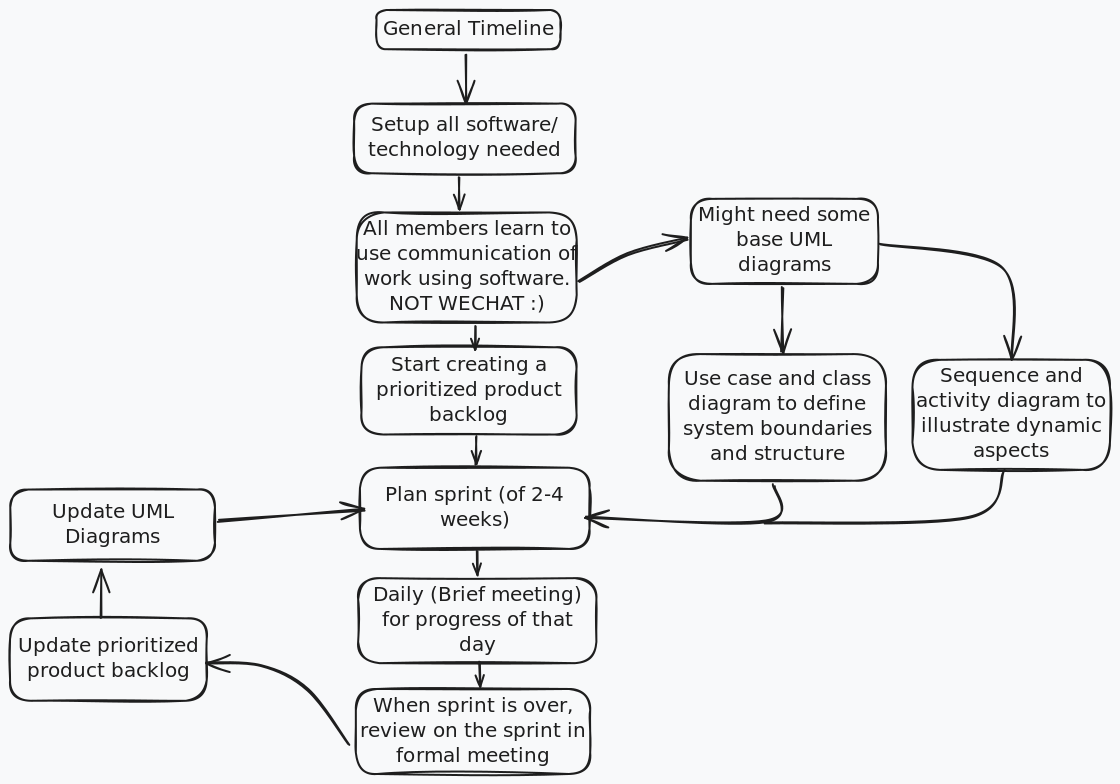
\includegraphics[width=\linewidth]{OtherImage/General_Workflow.png}
    \caption{General Workflow}
    \label{fig:general-workflow}
\end{figure}

The main workflow includes planning sprints, having daily meetings (stand ups), sprint reviews, and continuously updating product backlog and UML diagrams.\\

\newpage

\section{Updated Time Plan}

Figure \ref{fig:collapsed-gantt-chart}, shows a provisional Gantt Chart with all the details collapsed that will be updated as needed during the project. For the expanded Gantt chart, see Appendix \ref{sec:expanded-gantt-chart}. \\

\begin{figure}[H]
   \centering
    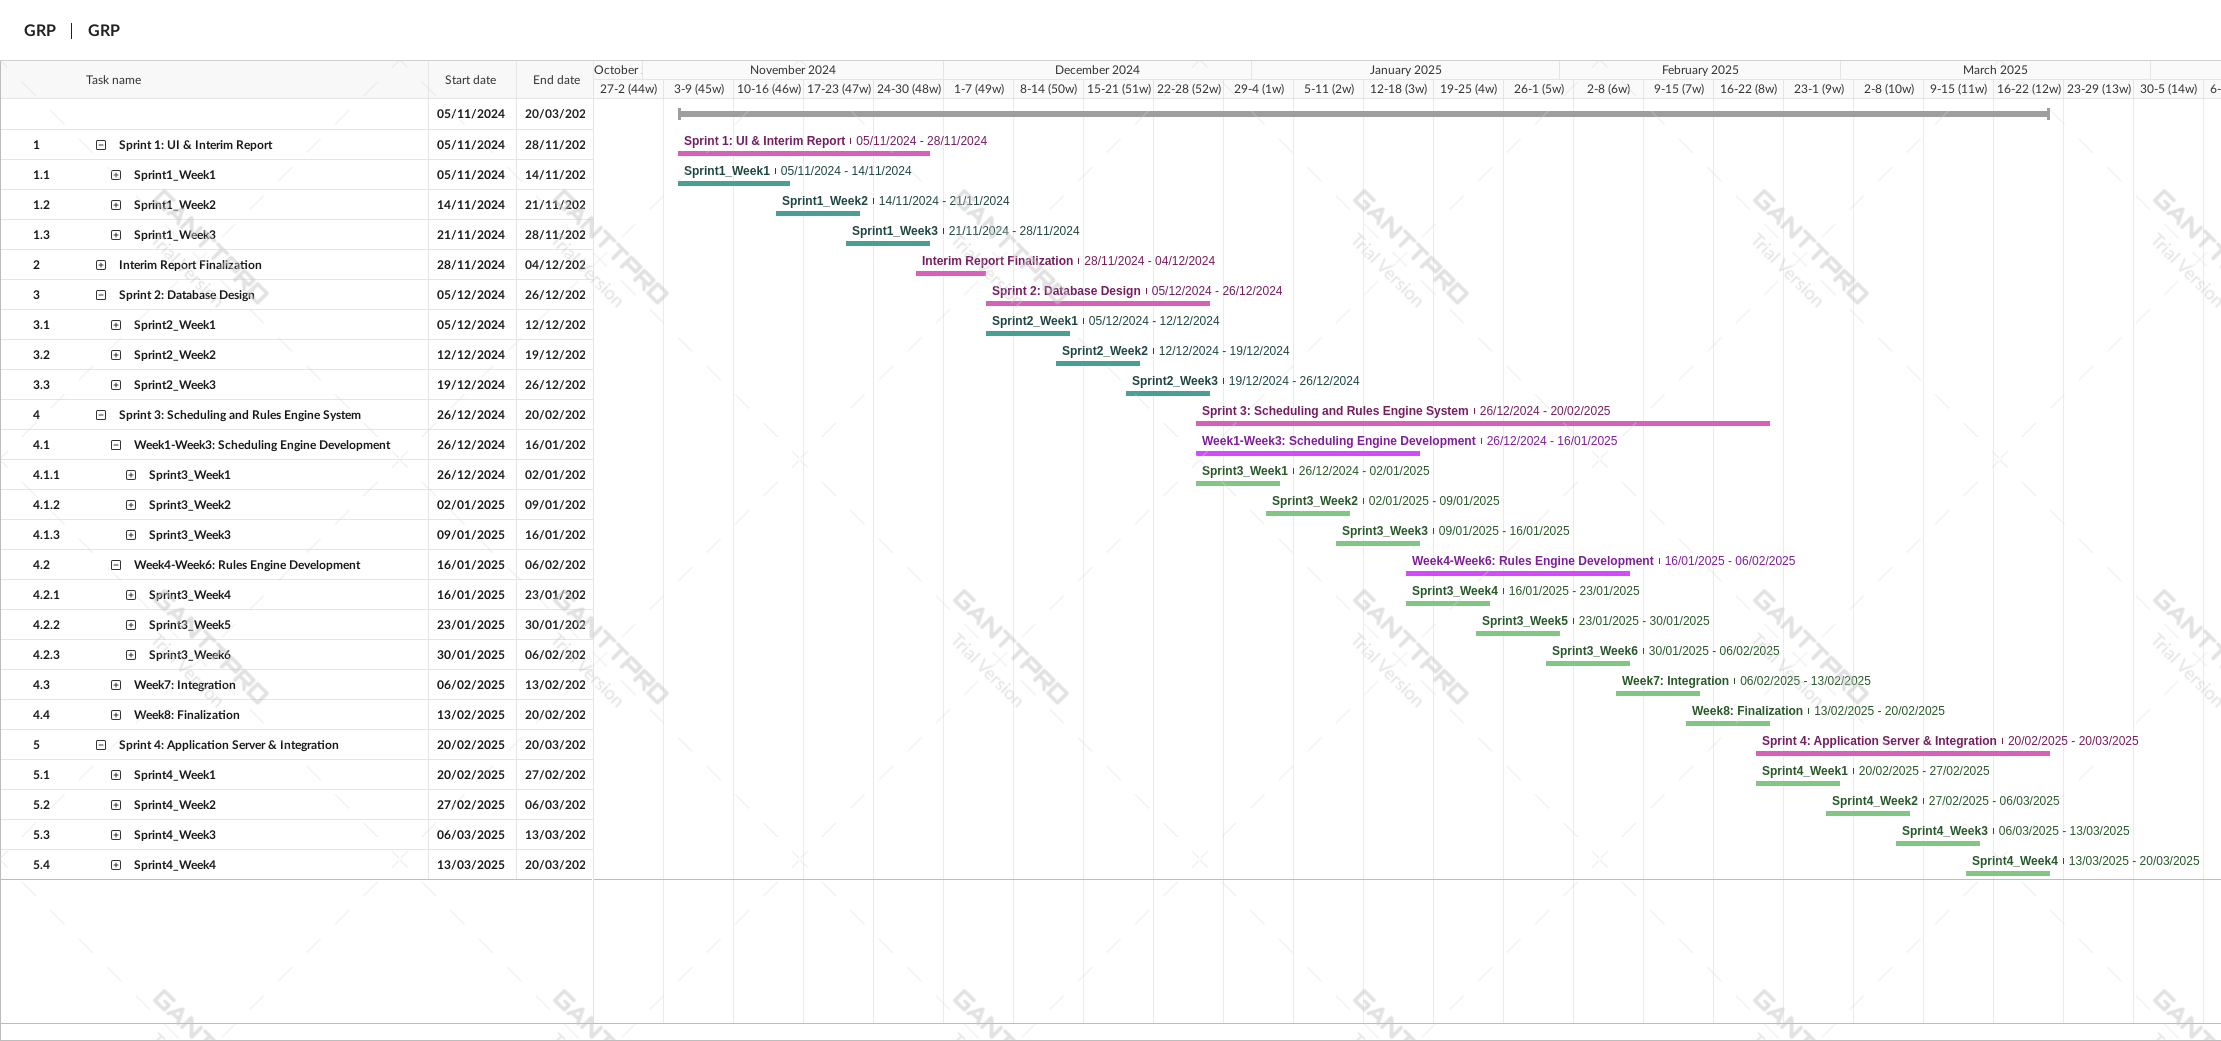
\includegraphics[width=\linewidth]{GanttCharts/GRP_GanttChart_Collapsed.png}
    \caption{Collapsed Gantt Chart}
    \label{fig:collapsed-gantt-chart}
\end{figure}


\subsection{Current Progress}
The first sprint from 5th November 2024 to 28th November 2024 ran successfully without any time extension needed. The first sprint was planned to complete the UI of the Web Application.\\

\subsection{Upcoming Phases}
The second sprint from 5th December 2024 to 26th December 2024 will focus on database design which includes setting up the database as well as designing the database schema. The third sprint from 26th December 2024 to 20th February 2025 will focus on developing the scheduling and rules system. The two systems are being developed simultaneously because of their close interdependence.\\

The final sprint from 20th February 2025 to 20th March 2025 will focus on building the main application server as well as its integration with the other systems like database, scheduling system, rules system, and the user interfaces. The final weeks of each sprint will be dedicated to integration testing and bug fixing, whilst TDD will be done where unit tests are taken place throughout the development process.\\

\phantomsection
\addcontentsline{toc}{chapter}{Bibliography}
\bibliographystyle{agsm}
\bibliography{references}

\begin{appendices}
\cleardoublepage
\chapter{Expanded Gantt Chart}
\label{sec:expanded-gantt-chart}
\begin{figure}[H]
    \includegraphics[width=0.8\textwidth]{GanttCharts/GRP_GanttGraph_Expanded_P1.png}
\end{figure}
\begin{figure}[H]
    \centering
    \includegraphics[width=\textwidth]{GanttCharts/GRP_GanttGraph_Expanded_P2.png}
\end{figure}
\begin{figure}[H]
    \centering
    \includegraphics[width=\textwidth]{GanttCharts/GRP_GanttGraph_Expanded_P3.png}
\end{figure}
\begin{figure}[H]
    \centering
    \includegraphics[width=\textwidth]{GanttCharts/GRP_GanttGraph_Expanded_P4.png}
\end{figure}
\chapter{Meeting Minutes}
\section{Meeting Minutes 1}
\begin{figure}[H]
    \centering
    \includegraphics[width=0.7\textwidth]{Minutes/Minutes_1-cropped-1.png}
\end{figure}
\newpage
\begin{figure}[H]
    \centering
    \includegraphics[width=\textwidth]{Minutes/Minutes_1-cropped-2.png}
\end{figure}
\newpage
\begin{figure}[H]
    \centering
    \includegraphics[width=\textwidth]{Minutes/Minutes_1-cropped-3.png}
\end{figure}
\newpage
\begin{figure}[H]
    \centering
    \includegraphics[width=\textwidth]{Minutes/Minutes_1-cropped-4.png}
\end{figure}
\section{Meeting Minutes 2}
\begin{figure}[H]
    \centering
    \includegraphics[width=\textwidth]{Minutes/Minutes_2-cropped-1.png}
\end{figure}
\newpage
\begin{figure}[H]
    \centering
    \includegraphics[width=\textwidth]{Minutes/Minutes_2-cropped-2.png}
\end{figure}
\newpage
\begin{figure}[H]
    \centering
    \includegraphics[width=\textwidth]{Minutes/Minutes_2-cropped-3.png}
\end{figure}
\section{Meeting Minutes 3}
\begin{figure}[H]
    \centering
    \includegraphics[width=\textwidth]{Minutes/Minutes_3-cropped-1.png}
\end{figure}
\newpage
\begin{figure}[H]
    \centering
    \includegraphics[width=\textwidth]{Minutes/Minutes_3-cropped-2.png}
\end{figure}
\newpage
\begin{figure}[H]
    \centering
    \includegraphics[width=\textwidth]{Minutes/Minutes_3-cropped-3.png}
\end{figure}
\newpage
\begin{figure}[H]
    \centering
    \includegraphics[width=\textwidth]{Minutes/Minutes_3-cropped-4.png}
\end{figure}
\newpage
\begin{figure}[H]
    \centering
    \includegraphics[width=\textwidth]{Minutes/Minutes_3-cropped-5.png}
\end{figure}

\section{Meeting Minutes 4}
\begin{figure}[H]
    \centering
    \includegraphics[width=\textwidth]{Minutes/Minutes_4-cropped-1.png}
\end{figure}
\newpage
\begin{figure}[H]
    \centering
    \includegraphics[width=\textwidth]{Minutes/Minutes_4-cropped-2.png}
\end{figure}
\newpage
\begin{figure}[H]
    \centering
    \includegraphics[width=\textwidth]{Minutes/Minutes_4-cropped-3.png}
\end{figure}
\newpage
\begin{figure}[H]
    \centering
    \includegraphics[width=\textwidth]{Minutes/Minutes_4-cropped-4.png}
\end{figure}
\section{Meeting Minutes 5}
\begin{figure}[H]
    \centering
    \includegraphics[width=\textwidth]{Minutes/Minutes_5-cropped-1.png}
\end{figure}
\newpage
\begin{figure}[H]
    \centering
    \includegraphics[width=\textwidth]{Minutes/Minutes_5-cropped-2.png}
\end{figure}
\section{Meeting Minutes 6}
\begin{figure}[H]
    \centering
    \includegraphics[width=0.9\textwidth]{Minutes/Minutes_6-cropped-1.png}
\end{figure}
\newpage
\begin{figure}[H]
    \centering
    \includegraphics[width=\textwidth]{Minutes/Minutes_6-cropped-2.png}
\end{figure}
\newpage
\begin{figure}[H]
    \centering
    \includegraphics[width=\textwidth]{Minutes/Minutes_6-cropped-3.png}
\end{figure}
\section{Meeting Minutes 7}
\begin{figure}[H]
    \centering
    \includegraphics[width=0.9\textwidth]{Minutes/Minutes_7-cropped-1.png}
\end{figure}
\newpage
\begin{figure}[H]
    \centering
    \includegraphics[width=\textwidth]{Minutes/Minutes_7-cropped-2.png}
\end{figure}

\end{appendices}


\end{document}


